\documentclass[12pt]{report}

% All packages imported
\usepackage[french,english]{babel}
\usepackage{caption}
\usepackage[utf8]{inputenc}
\usepackage{csquotes}
\usepackage[T1]{fontenc}
\usepackage[margin=1in]{geometry}
\usepackage{graphicx}
\usepackage{setspace}\doublespacing
\usepackage[colorlinks=true, linkcolor=blue, citecolor=teal]{hyperref}
\usepackage{stix2}
\usepackage{titlecaps}
\usepackage{xcolor}
\usepackage{xparse}

\usepackage[authordate,backend=biber,sorting=nty]{biblatex-chicago}
\bibliography{references}
\renewcommand*{\bibfont}{\normalfont\footnotesize}

% The stopwords to remove from titlecase
\Addlcwords{i me my myself we our ours ourselves you your
yours yourself yourselves he him his himself she her hers
herself it its itself they them their theirs themselves
what which who whom this that these those am is are was
were be been being have has had having do does did doing
a an the and but if or because as until while of at by
for with about against between into through during
before after above below to from up down in out on
off over under again further then once here there
when where why how all any both each few more most
other some such no nor not only own same so than
too very can will just don should now vs}


% This is a workaround for a "token not allowed" issue
\newcommand{\titlecapwrap}[1]{
    \texorpdfstring{\titlecap{#1}}{#1}
}

% The command to remove spaces
% Amazing trick to remove spaces betwen words by:
% https://tex.stackexchange.com/questions/87509/removing-the-spaces-between-words
\makeatletter
\def\RemoveSpaces#1{\zap@space#1 \@empty}
\makeatother

% The definitions for the Roman numeral syntax
\newcommand{\rnformat}[1]{\textbf{#1}\relax}
\newcommand{\rn}[1]{\rnformat{#1}\relax}
\newcommand{\rndim}{{\footnotesize {}^\rnformat{o}{}\relax}}
\newcommand{\rnhdim}{{\footnotesize{}^\rnformat{\o}{}\relax}}
\newcommand{\rnseven}{{\footnotesize {}^\rnformat{7}\relax}}
\newcommand{\rnsix}{{\footnotesize {}^\rnformat{6}\relax}}
\newcommand{\rnsixfour}{{\footnotesize{}^\rnformat{6}_\rnformat{4}\relax}}
\newcommand{\rnsixfive}{{\footnotesize{}^\rnformat{6}_\rnformat{5}\relax}}
\newcommand{\rnfourthree}{{\footnotesize{}^\rnformat{4}_\rnformat{3}\relax}}
\newcommand{\rntwo}{{\footnotesize {}^\rnformat{2}\relax}}

% The shortcuts for figures with less code
\NewDocumentCommand{\phdfigure}{ O{Caption placeholder}
O{0.6} O{h!} m}{
    \begin{figure}[#3]
        \centering
        \includegraphics[width=#2\textwidth]{chapters/\arabic{chapter}/figures/#4}
        \caption{#1.}
        \label{fig:#4}
    \end{figure}
    \relax
}

\NewDocumentCommand{\phdtwofigures}{ O{Caption1 placeholder}
O{Caption2 placeholder} O{0.5} O{0.5} m m}{
\begin{figure}[h!]
    \centering
    \begin{minipage}{#3\textwidth}
      \centering
      \includegraphics[width=0.9\linewidth]{chapters/\arabic{chapter}/figures/#5}
      \captionof{figure}{#1.}
      \label{fig:#5}
    \end{minipage}%
    \begin{minipage}{#4\textwidth}
      \centering
      \includegraphics[width=0.9\linewidth]{chapters/\arabic{chapter}/figures/#6}
      \captionof{figure}{#2.}
      \label{fig:#6}
    \end{minipage}
    \end{figure}
    \relax
}


\NewDocumentCommand{\phdthreefigures}{ O{Caption1
placeholder} O{Caption2 placeholder} O{Caption3 placeholder}
O{0.33} O{0.33} O{0.33} m m m}{
\begin{figure}[h!]
    \centering
    \begin{minipage}{#4\textwidth}
      \centering
      \includegraphics[width=0.9\linewidth]{chapters/\arabic{chapter}/figures/#7}
      \captionof{figure}{#1.}
      \label{fig:#7}
    \end{minipage}%
    \begin{minipage}{#5\textwidth}
      \centering
      \includegraphics[width=0.9\linewidth]{chapters/\arabic{chapter}/figures/#8}
      \captionof{figure}{#2.}
      \label{fig:#8}
    \end{minipage}%
    \begin{minipage}{#6\textwidth}
      \centering
      \includegraphics[width=0.9\linewidth]{chapters/\arabic{chapter}/figures/#9}
      \captionof{figure}{#3.}
      \label{fig:#9}
    \end{minipage}
    \end{figure}
    \relax
}

% Other shortcuts for an easier workflow


\newcommand{\phdtable}[1]{\input{chapters/\arabic{chapter}/tables/#1.tex}}
\newcommand{\phdinput}[1]{\input{chapters/\arabic{chapter}/#1.tex}}

\newcommand{\phdchapter}[1]{\chapter{\titlecapwrap{#1}}\label{chap:\RemoveSpaces{#1}}}
\newcommand{\phdsection}[1]{\section{\titlecapwrap{#1}}\label{sec:\RemoveSpaces{#1}}}
\newcommand{\phdsubsection}[1]{\subsection{\titlecapwrap{#1}}\label{sec:\RemoveSpaces{#1}}}
\newcommand{\phdsubsubsection}[1]{\subsubsection{\titlecapwrap{#1}}\label{sec:\RemoveSpaces{#1}}}
\newcommand{\phdparagraph}[1]{\paragraph{\titlecapwrap{#1}}\label{par:\RemoveSpaces{#1}}}

\newcommand{\refchap}[1]{\hyperref[chap:#1]{Chapter~\ref*{chap:#1}}}
\newcommand{\refsec}[1]{\hyperref[sec:#1]{Section~\ref*{sec:#1}}}
\newcommand{\refpar}[1]{\hyperref[par:#1]{Paragraph~\ref*{par:#1}}}
\newcommand{\reffig}[1]{\hyperref[fig:#1]{Figure~\ref*{fig:#1}}}
\newcommand{\reftab}[1]{\hyperref[tab:#1]{Table~\ref*{tab:#1}}}
\newcommand{\refeq}[1]{\hyperref[eq:#1]{Equation~\ref*{eq:#1}}}

% A few formatting macros
\newcommand{\code}[1]{\texttt{#1}}

\newcommand{\missing}[1]{{\color{red} A #1 will be inserted here}}
% \newcommand{\guide}[1]{{\color{gray}\textbf{#1}}}
\newcommand{\guide}[1]{}


\setcounter{tocdepth}{3}
\setcounter{secnumdepth}{3}

\begin{document}

% COMPILE A SINGLE CHAPTER. Comment for full thesis
\def\compilechapter{8}

\ifx\compilechapter\undefined
    \pagenumbering{roman}
    \begin{titlepage}
\begin{center}
    % \vspace*{1cm}

    \huge
    \textbf{Automatic Roman numeral analysis in symbolic music representations}

    % \vspace{0.5cm}
    % An approached based on Convolutional Recurrent Neural Networks

    \vspace{1cm}

    \LARGE
    N\'estor N\'apoles L\'opez

    \vspace{1cm}

    
\includegraphics[width=0.2\textwidth]{./figures/mcgill}

    \vspace{0.5cm}

    \large
    Music Technology Area \\
    Department of Music Research \\
    Schulich School of Music \\
    McGill University, Montr\'eal \\

    \vfill

    April 2022

    \vspace{2cm}

    A thesis submitted to McGill University in partial fulfillment of the requirements of the degree of Doctor of Philosophy

    \vspace{1cm}

    \textcopyright \ N\'estor N\'apoles L\'opez 2022

\end{center}
\end{titlepage}

    \tableofcontents{}
    \chapter*{Abstract}
\addcontentsline{toc}{chapter}{Abstract}
\label{chap:chap0-abs}

One of the most common ways to analyze a piece of tonal
music is through Roman numeral analysis. This requires the
inspection of several attributes related to chords and keys.
Chords can be inspected in terms of their properties: root,
quality, inversion, and function. Keys can be inspected in
terms of their temporal scope as modulations or
tonicizations. Each of these attributes (or tasks) of Roman
numeral analysis can be modeled in isolation. However,
recent research has found that analyzing several tonal tasks
simultaneously leads to more robust MIR models. This has
motivated the research of multitask models for Roman numeral
analysis. In this dissertation, I extend this line of
research by: (1) improving the data-curation process for
existing datasets; (2) developing a new data-augmentation
technique for Roman numeral analysis models; (3) improving
the design of existing convolutional recurrent neural
networks; and (4) extracting more tonal tasks from the Roman
numeral annotations. Combining these ideas, I trained a new
Roman numeral analysis model. Among other applications, this
will facilitate advanced searching in music collections. For
example, searching by chord progressions or by modulation
trajectories.

    \chapter*{R\'esum\'e}
\addcontentsline{toc}{chapter}{R\'esum\'e}
\label{chap:chap0-res}

L'une des façons les plus courantes d'analyser un morceau de musique tonale est l'analyse des chiffres romains.
Cela nécessite l'inspection de plusieurs attributs liés aux accords et aux tonalités.
Les accords peuvent être inspectés en fonction de leurs propriétés : racine, qualité, inversion et fonction.
Les clés peuvent être inspectées en termes de leur portée temporelle comme les modulations ou les tonifications.
Chacun de ces attributs (ou tâches) de l'analyse des chiffres romains peut être modélisé de manière isolée.
Cependant, des recherches récentes ont montré que l'analyse simultanée de plusieurs tâches tonales conduit à des modèles MIR plus robustes.
Ceci a motivé la recherche de modèles multitâches pour l'analyse des chiffres romains.
Dans cette thèse, je développe cette ligne de recherche en :
(1) améliorant le processus de curation des données pour les ensembles de données existants ;
(2) développant une nouvelle technique d'augmentation des données pour les modèles d'analyse des chiffres romains ;
(3) améliorant la conception des réseaux neuronaux récurrents convolutionnels existants ;
et (4) l'extraction de plus de tâches tonales à partir des annotations de numéraux romains.
En combinant ces idées, j'ai formé un nouveau modèle d'analyse des numéraux romains.
Entre autres applications, cela facilitera la recherche avancée dans les collections de musique.
Par exemple, la recherche par progression d'accords ou par trajectoires de modulation.
    \chapter*{Acknowledgements}
\addcontentsline{toc}{chapter}{Acknowledgements}
\label{chap:chap0-ack}

I will first and foremost thank my PhD advisor, Ichiro
Fujinaga. For the most part of my PhD, Ichiro scheduled
weekly meetings with me that were of the utmost help.
Together, we walked through machine-learning prototypes,
presentations, code, music theories, and papers. Research
aside, Ichiro has been a supportive friend since I moved to
Montr\'eal. Thank you, Ich.

Secondly, I would like to thank my family, who have
supported me all along my journey of pursuing my dreams: my
spouse and best friend, Kinga; my parents, Martha and
Eduardo; my siblings, Grecia, Eric, and sister-in-law
Fabiola; and my parents in law, Gra\.zyna and Miros\l{}aw.

After my advisor, my co-authors provided me with many ideas
and feedback related to the research presented here. Thanks
to all of you: Gabriel Vigliensoni, Claire Arthur, Laurent
Feisthauer, Florence Lev\'e, Mark Gotham, and the
Computational Tonal Studies group.

While in Montr\'eal, I met a group of extraordinary people
that made my stay much more pleasant and enriching. Thanks
to all the members of the DDMAL and CIRMMT communities, but
particularly, thanks to Gabriel Vigliensoni, Martha Thomae,
Matan Gover, Yulia Draginda, Yuval Adler, Alex Daigle, Emily
Hopkins, Yaolong Ju, Timothy de Reuse, Sylvain Margot, Jacob
Sanz-Robinson, K\'e Zhang, and Erica Huynh.

Thanks to McGill professors Julie Cumming, Peter Schubert,
William Caplin, Jon Wild, Philippe Depalle, Marcelo
Wanderley, and Gary Scavone, from whom I learned different
aspects of music and technology that contributed explicitly
or implicitly to the work presented in this dissertation.

Thanks to other members of the global music information
retrieval and computational musicology communities,
particularly, Craig Sapp, Michael Scott Cuthbert, Jacob
Tyler Walls, Reinier de Valk, Emilia Parada-Cabaleiro, and
others with whom I shared code, papers, and conversations.

The research presented in this dissertation would not have
been possible without the generous support of different
institutions. The \emph{Fonds de recherche --- Soci\'et\'e
et culture} (FRQSC), from which I obtained a doctoral
scholarship from 2019--2022 (dossier number 271479); the
\emph{Centre for Interdisciplinary Research in Music Media
and Technology} (CIRMMT), from which I obtained several
travel awards and a student project award; the SIMSSA
project, from which I received a generous stipend during the
first two years of my PhD (2017--2018) and a role as a
casual research assistant for the remainder of my PhD; the
Schulich School of Music, from which I received additional
travel and conference registration awards. Thank you to all
these wonderful organizations and their commitment to music
research.

Thanks to people who had an early influence in me and helped
me to set my current path: Luis Alberto Casillas
Santill\'an, Abelardo Guti\'errez, Juan Jos\'e L\'opez
Sandoval, Nancy Arana Daniel, Sergio Bola\~nos, Leo Hendrik
Reyes, and Juan Rodrigo P\'erez C\'ardenas.

Lastly, my friends, for being always there: Jhonnatan Razo,
Dulce Alcal\'a, and El\'i Lezama. ¡Gracias, amigos!

    \pagenumbering{arabic}
    \phdchapter{introduction}

% \begin{quote}
%     A quote
% \end{quote}
% \clearpage

% Taken verbatim from thesis proposal

\guide{Problem.}
One of the most common ways to analyze a piece of tonal
music is through Roman numeral analysis. This requires the
inspection of several attributes related to chords and keys.
Chords can be inspected in terms of their properties: root,
quality, inversion, and function. Keys can be inspected in
terms of their temporal scope as modulations or
tonicizations~\parencite{napoles_lopez2020local}. Each of
these attributes (or tasks) of Roman numeral analysis can be
modeled in isolation. As a result, many models for automatic
key and chord analysis exist in the Music Information
Retrieval (MIR) literature. Recent research has found that
analyzing several tonal tasks simultaneously leads to more
robust MIR models. This happens via multitask learning, a
technique where a machine learning model solves several
problems at once~\parencite{ruder2017overview}. This has
motivated the research of multitask models for Roman numeral
analysis. However, even the best of the models has
significant limitations. For example, recent models output
the correct Roman numeral annotation $\sim$42\% of the
times~\parencite{chen2021attend, micchi2020not}.

\guide{Proposal.}
Here, I propose to address existing limitations in multitask
Roman numeral analysis models. In particular, I will focus
on four improvements: (1) to standardize the syntax and
quality across various existing Roman numeral analysis
datasets; (2) to investigate new data-augmentation
techniques that overcome the scarcity of expert-annotated
data; (3) to enhance the design of neural network
architectures for Roman numeral analysis; and (4) to explore
different combinations of tonal tasks in multitask learning
configurations.

Combining these ideas, I trained a new Roman numeral
analysis model. The resulting model is capable of annotating
large amounts of symbolic music files with Roman numeral
labels. Among other applications, this facilitates searching
in music collections. For example, searching by chord
progressions or by modulation trajectories.

\phdsection{motivation}
    % Taken verbatim from thesis proposal

\guide{Introduction.}
In this scientific and cultural age, it is not difficult to
defend the use of computers for studying any field,
including music. We expect computers to automate much of our
``chores'', annotate large volumes of data that we can not
possibly annotate, and democratize the access to resources
beyond the wealthy societies to create more fair
opportunities for every human being to receive education and
pursue their passions, including music.

Yet, I would not like to start this thesis by making an
argument about how the development of an automated tonal
analysis machine is going to annotate large volumes of music
for us, as important as that application may be.

What I want to suggest, at first and overall, is that music
is a very complex, highly-dimensional phenomenon. As such,
our efforts to explain or simplify its underlying logic will
break at one point or another. Particularly, I see Western
classical music as an example of those efforts for
simplification and collective intelligibility; the evolution
of the Common Western Music Notation system, and the
evolution of the harmonic theories that have facilitated the
explanation of what composers of the canon have done. Giving
names to the conventions, patterns, and structures that
repeat and become familiar to the listener and the music
composer.

Music theory fails, in the sense that it is only as good as
it is able to explain conventions, patterns, and structures
of all existing music.

\dots something here

% Bring example of "augmented unison" in the Huron rules and
% a chromatic passage where it doesn't work

\textcite{huron2016voice} summarized voice leading
rules.\footnote{See Chapter~2.} Among these rules, there is
one on the forbidden augmented and diminished melodic
intervals. Although this rule seems consistent with the
expected practice of voice leading, it demonstrates to break
in passages with chromatic basslines. That is, a chord
progression with a chromatic line \textbf{requires} an
augmented unison to achieve the best voice leading possible.
Coming up with rules that work for every scenario is nearly
impossible. Testing them in a computer algorithm is
feasible, however.

\dots something here

\guide{Why do we study these things computationally.}
The reason why I think it is important to study tonality
computationally is because music easily evokes human bias.
It is easy to summon the personal bias when listening to a
piece of music. Likewise, when analyzing a piece of music. I
like to think of computer algorithms as unbiased judges of
the theory. Emotionless, deterministic. If the theories
generalize well to the musical repertoire, it will show in
the output of an algorithm. If not, it is likely that the
output will reveal where the theory fails to explain the
musical phenomenon.
% In this thesis, it is my intention not only to present my
% experiments designing a neural network for tonal music
% analysis, but also the interpretation of the results. For
% example, when a state-of-the-art neural network is trained
% to recognize modulations, what is it that the internal
% representations of the network (i.e., the hidden layers)
% are learning? To my knowledge, this aspect is generally
% less explored in machine learning literature, where the
% focus is on improving the evaluation metrics of new
% algorithms versus old algorithms. As a theorist, I want to
% know what is it that the ruthless optimization method is
% learning when it provides meaningful outputs of tonal
% music analysis.
I suggest that to be the reason why computers are and should
be the companion of old and new music theories. They help us
to test our assumptions in practical scenarios, in unbiased
ways and faithful to the formulations in the theory.

The multitask tonal analysis done here, although it consists
of multiple tasks, is focused around two specific problems:
chord analysis and key analysis. These problems have been
studied thoroughly in isolation and, sometimes, in
conjunction.


\guide{Problem.}
One of the most common ways to analyze a piece of tonal
music is through Roman numeral analysis. This requires the
inspection of several attributes related to chords and keys.
Chords can be inspected in terms of their properties: root,
quality, inversion, and function. Keys can be inspected in
terms of their temporal scope as modulations or
tonicizations~\parencite{napoleslopez2020local}. Each of
these attributes (or tasks) of Roman numeral analysis can be
modeled in isolation. As a result, many models for automatic
key and chord analysis exist in the Music Information
Retrieval (MIR) literature. Recent research has found that
analyzing several tonal tasks simultaneously leads to more
robust MIR models. This happens via multitask learning, a
technique where a machine learning model solves several
problems at once~\parencite{ruder2017overview}. This has
motivated the research of multitask models for Roman numeral
analysis. However, even the best of the models has
significant limitations. For example, recent models output
the correct Roman numeral annotation $\sim$42\% of the
times~\parencite{chen2021attend, micchi2020not}.

\guide{Proposal.}
Here, I propose to address existing limitations in multitask
Roman numeral analysis models. In particular, I will focus
on four improvements: (1) to standardize the syntax and
quality across various existing Roman numeral analysis
datasets; (2) to investigate new data-augmentation
techniques that overcome the scarcity of expert-annotated
data; (3) to enhance the design of neural network
architectures for Roman numeral analysis; and (4) to explore
different combinations of tonal tasks in multitask learning
configurations.

Combining these ideas, I trained a new Roman numeral
analysis model. The resulting model is capable of annotating
large amounts of symbolic music files with Roman numeral
labels. Among other applications, this facilitates searching
in music collections. For example, searching by chord
progressions or by modulation trajectories.

\phdsection{why key finding}
    % Taken verbatim from comps Q5

% Across the literature, the most mentioned application of
% key-finding algorithms is its use in \emph{harmonic
% mixing} applications for DJs. There are companies that
% value accurate and automatic annotations of the musical
% key for this purpose. However, as described in audio
% feature taxonomies, a musical key is also a feature that
% characterizes a musical fragment. Its presence (tonal
% music) or absence (modal or atonal music), its strength
% (highly harmonic vs. highly contrapuntal), and its change
% over time (intermediate keys, modulations) can tell us
% valuable information about a piece of music and its
% characteristics. When analyzed from a multitude of
% viewpoints, it has been shown by Sapp that different music
% create very different tonal visualizations, or as he calls
% them, \emph{keyscapes}.

% We refer to key-finding as the process of determining the
% key of a musical piece, for example, the key that is
% written on the title of the piece.

% Furthermore, a key-finding model is an algorithm that
% allows us to determine that key automatically given a
% digital representation of the piece of music (see Question
% \ref{chap:chap4} for a more extensive review of digital
% representations of music).

% Over the years, multiple applications have emerged for
% these type of systems. These applications can be divided
% in the applications of \emph{global} key-finding
% algorithms and \emph{local} key-finding algorithms (see
% Question \ref{chap:chap6} for a further discussion on
% global and local keys).

% \todo[inline]{Locate applications based on the papers for
% this question}

% \guide{Global key-finding applications}

% Some of the utilities of key-finding algorithms are music
% classification, music cataloguing, and harmonic mixing for
% DJs.

% These applications appear frequently across the literature
% of key-finding models.

% \guide{Local key-finding applications}

% Although not as frequently mentioned as the applications
% of global keys, researchers have also found useful
% applications for local key-finding models across the field
% of Music Information Retrieval. \begin{enumerate} \item
% Structural segmentation of the music \item Roman numeral
% analysis \item Pitch-spelling algorithms \item Chord
% labeling \item Visualizing tonality in music
% \end{enumerate}

% % One problem that most of these applications of local
% key-finding models share is that local keys are very
% difficult to evaluate quantitatively, that is,
% empirically, we know that keys are related with chords,
% the spelling of the notes, functional harmony, and musical
% structure, but we do not know how much and that is very
% difficult to know

% Local key-finding models and their applications are,
% nevertheless, less common. Mainly, because local
% key-finding models are very difficult to evaluate. On the
% other hand, global key-finding models are relatively
% easier to evaluate quantitatively, and have become more
% popular over the years.

% \guide{Going further into new research questions}

% Sapp \parencite{sapp2011computational} studied tonality through
% the computation of a key-finding model at different window
% lengths of a piece of music.

% From the tonal regions obtained, he categorized different
% regions as either chords, tonicizations, and modulations.

% How do we know this is true?

% \begin{figure}[h] \centering
%     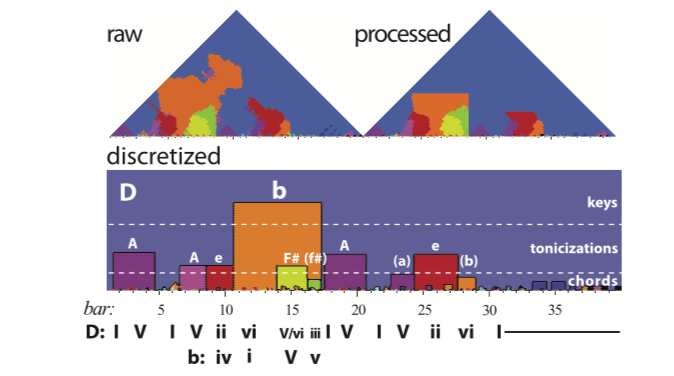
\includegraphics[width=0.6\textwidth]{figures/Q5_1.png}
%     \caption{Key-finding algorithm used to delimit chords,
%     tonicizations, and modulations in a piece of music}
%     \label{fig:Q5_1} \end{figure}

% \guide{Concrete questions that we can ask in a symbolic
% music corpus}

% How many changes of key (modulations) happen in a given
% piece? How many tonicizations happen in a given piece? How
% many of those would be annotated by a human annotator? How
% many of those overlapped or mismatched between annotators?
% How many of those were found by local key-finding
% algorithms? How many of those end in a Perfect Authentic
% Cadence or confirm other structural cues mentioned in
% music theory for modulations? How many times does the
% local key mismatches the global key of the beginning of
% the piece? How many times does the local key mismatches
% the global key of the end of the piece?

% \guide{Interesting properties of musical keys in the study
% of tonality}

% What does evaluation has to do with any of this? I should
% be really talking about applications.

After the first attempt of designing a key-finding algorithm
by Longuet-Higgins \parencite{longuethiggins1971interpreting},
many algorithms have followed throughout the years. These
algorithms, using different approaches and methodologies,
attempt to retrieve the key of digital music representations
in the symbolic and audio domains (see Question
\ref{chap:chap3} for a survey on key-finding models).

The problem of designing an algorithm that is able to
retrieve musical keys, among other tonal features, has also
been the motivation of several dissertations
\parencite{gomez2006tonal, campbell2010automatic,
korzeniowski2018harmonic, sapp2011computational,
chew2000towards}.

During the research literature, the applications for
key-finding models are often discussed and a few examples
are frequently mentioned: the possibility of indexing large
volumes of music by their musical key in digital music
libraries; the automatic annotation of music data available
on the web, which does not usually include the annotation of
the musical key; and the reliable extraction of musical keys
as machine learning features, which have been shown to be
useful in other Music Information Retrieval (MIR) tasks
\parencite{mauch2010approximate, chai2005detection}. Another
application, particularly interesting for those pursuing the
commercial viability of key-finding models, comes
surrounding certain music communities, for example,
Electronic Dance Music (EDM), where the knowledge of the key
can be very helpful for performers during the mixing
process, given that a common technique involves mixing music
with similar harmonic structures, a technique known as
\emph{harmonic mixing}. This necessity opens a commercial
opportunity for the designers of key-finding models, given
that companies profit from having reliable annotations that
they can offer to their users.

Nevertheless, aside from the necessity of key-finding models
in digital libraries and commercial applications,
researchers have also encountered themselves (maybe as a
byproduct of research and design decisions), with
interesting musicological questions. Here, I decide to
concentrate on those, formulating a few questions based on
the research inquiries, claims, and assumptions that can be
found surrounding the literature of key-finding
algorithms.\footnote{Unless explicitly mentioned, the
questions listed here are not direct quotes from the cited
papers but questions formulated given
a---sensible---interpretation of the statements in the cited
papers. Following the question, comes a discussion of the
paper (and the context) from which the question was
formulated.}

\guide{Questions regarding the study of key-finding algorithms}

\textbf{\emph{What is the field that studies musical keys
and tonality?}}

According to Vos \parencite{vos2000tonality}, there is a natural
``bias'' in the scientific study of tonality, due to the
interdisciplinarity of the problem and the fact that no
person is specialized in music theory, music history,
psychoacoustics, music psychology, and computer science. All
at the same time. If there is a person with such a
background, certainly the expertise in each area is
asymmetrical, which leads to a biased view of the problem
towards the area where the researcher has more expertise.
This has a noticeable effect in the research of key-finding
algorithms, as a successful algorithm for finding musical
keys \parencite{korzeniowski2018harmonic}  could reduce its
discussion on musical implications of keys, tonality,
harmonic tension, and ambiguity to a negligible part of the
research document, completing the rest of the document with
thorough, well-designed experiments of machine learning and
statistical analysis, typical of computer science but
difficult to find in any music-theoretical study. Krumhansl
revisits this issue \parencite{krumhansl2004cognition}, surveying
studies from multiple disciplines that try to explain what
tonality is (musical keys included), according to different
perspectives. In that study, Krumhansl dedicates a section
to discuss the point of view of music cognition, acoustics,
musicology, computer science, music theory, and brain
science.

In a very different---almost comedic---work, Aucouturier and
Bigand also touch on the issues of interdisciplinarity
\parencite{aucouturier2012mel}.

\textbf{\emph{Can we use key-finding algorithms as
``debugging'' tools for testing music theories? For example,
can we use them to observe the difference between a
modulation and a tonicization?}}

In his dissertation, Sapp introduced the \emph{keyscapes}
\parencite{sapp2011computational}, which allow the computation of
key-finding algorithms at different window sizes in a music
score and, moreover, visualizing the resulting output. He
claims that such visualization techniques can be useful as
evaluation tools, for example, by visually assessing the
strengths and weaknesses of a particular algorithm.
Additionally, Sapp claims that such visualization tools can
also be used to find the distinction between a modulation
and a tonicization, as tonicizations (in his proposed
visualization technique) do not extend towards the top end
of the \emph{keyscape}, while true modulations do. This
brings an interesting point, as there is no easy way to
quantitatively distinguish a modulation from a tonicization,
however, claiming that such visualization tools can do it
opens up the door to further musicological inquiries about
the concepts of modulation and tonicization, and their
scientific evaluation.


\textbf{\emph{When did tonality ``start''? And, did the
establishment of ``tonal music'' had something to do with
the refinement of temperament?}}

In the same paper discussed previously
\parencite{vos2000tonality}, Vos argues that one of the root
causes in the ``fuzziness'' of the term \emph{tonality} and
what it refers to, is that there is no clear boundary of
when and where that term should be applied historically. He
claims that tonality may be found in medieval folk songs and
Palestrina's ``modal counterpoint'', and at the same time,
examples by Bach can be interpreted as ``modal music''. If
that is true, how can we know whether the data used for
training and testing key-finding models is an accurate
representation of \emph{tonal} music explained by a major or
minor key.

In a different statement, Vos argues that one factor that
could have contributed significantly to the establishment of
"tonal music" is the refinement of temperament in the 18th
century. Temperament \emph{incentivized} modulation and
became a norm in Bach and subsequent composers. If used for
analyzing a representative sample of music compositions, a
reliable local-key-finding algorithm could be used for
addressing this question.

\textbf{\emph{Can we use key-finding evaluations as a metric
to evaluate the capability of spatial representations of
music?}}

In her dissertation \parencite{chew2000towards}, Chew introduced
a spatial representation of tonality, which consists of
multiple dimensions and allowed the computation of keys and
chords by locating them in such tonal space. This approach
has been followed by other researchers who have proposed
other spatial representations of tonality
\parencite{harte2006detecting}. Such representations are very
difficult to assess by humans, however, using computational
approaches to predict the key or chords in a musical excerpt
could be a useful way of measuring their validity. This
encourages the collection and annotation of data, which is
the same data used for designing and evaluating key-finding
algorithms. Additionally, having a reliable spatial
representation of tonality would mean understanding better
how tonality works.

\textbf{\emph{Does having the knowledge of the key changes
throughout a musical piece reveal the structure of the
piece?}}

In their study, Chai and Vercoe \parencite{chai2005detection}
found that in the self-similarity matrix of a piano sonata
by Mozart, with no apparent repetitions, the repetitions
became obvious as soon as the information of key changes
were introduced. Of course, this information would not
always yield favorable results, but it could help finding
structure in certain musical forms, like sonata-allegro
movements.

\textbf{\emph{Can the frequency of chords inform us about
the relationship between chords and keys?}}

Using the chord frequencies annotated in Budge's
dissertation \parencite{budge1943study}, Bellmann
\parencite{bellmann2006about} designed a \emph{key profile} to be
used with a new key-finding algorithm. The resulting
key-finding algorithm outperformed the accuracy of the
Krumhansl-Schmuckler algorithm
\parencite{krumhansl1990cognitive}, using solely information
about chord progressions.

Regarding how the key-finding algorithms should process the
musical inputs, Quinn has explicitly pointed out a few
questions that, through observation, seem as much of a
musicological nature as they seem of an engineering nature
\parencite{quinn2010are}. Quinn considers that these questions
``dominate'' the key-finding literature and the choices done
by researchers on the field: ``\textbf{\emph{Should window
size be defined in terms of chronological time, notational
(metrical) time, or number of note onsets? How big should
the window be? How does key-finding for a given window take
into account results for previous windows? How should
pitch-class distributions be weighted? How is a key
determination made from a given pitch-class
distribution?}}''

Finally, in a data-driven study by White and Quinn
\parencite{white2018chord}, a Hidden Markov Model (HMM) was given
the freedom to learn harmonic functions from Bach chorales,
examples of the Kostka-Payne harmony textbook, and the
McGill Billboard dataset. This process followed mostly an
unsupervised approach, without the explicit involvement of
the human experts deciding which functions needed to be
learnt by the model. As a result, the model came up with
different architectures for each type of music, sometimes
defying the expectations of music theory, and sometimes, at
least partially, validating them. This poses the following
question: \textbf{\emph{can we use key-finding and chord
recognition models, to propose new music theories?}}

    \phdsubsection{why local keys}
        % Taken verbatim from On Local Keys, Modulations, and
% Tonicizations

In some contexts such as guitar tablatures
\cite{ultimateguitar} and electronic dance music
\cite{beatport}, global-key annotations are useful as one of
the search parameters of a digital music library. Local-key
annotations, however, have not yet been used for this
purpose. It would be useful to complement key-related
searches with local-key annotations, using them to search
for musical pieces, based on their underlying changes of
key. As modulation are powerful tools to change the mood of
a score, indexing local keys within the score could help the
musicologist make bridges between lyrics and the tonal path.
However, the ``interpretability'' of local-key annotations
requires some attention first.

\phdsection{thesis structure}
    % Copyright 2021 Néstor Nápoles López

\refchap{introductiontoromannumeralanalysis}
introduces \gls{rna}, its history and
digitization. \refchap{background} introduces the relevant
research around music information retrieval for tonal music
analysis. \refchap{dataacquisitionandpreparation} introduces
the datasets and \gls{mlops} employed to train the Roman
numeral analysis model presented in this thesis.
\refchap{modeldesign} presents the design choices of the
convolutional recurrent neural network: number of layers,
multitask configuration, input and output representations,
etc. \refchap{experimentalevaluation} presents the
evaluation of the model against the state-of-the-art in
\glspl{rna}. \refchap{conclusions}
summarizes the main findings and presents closing remarks on
the current state of automatic tonal analysis and future
directions in the field.


    \phdchapter{introduction to roman numeral analysis}

% \begin{quote} A quote \end{quote} \clearpage

\phdinput{introduction_to_roman_numerals}
\phdsection{roman numeral analysis and chord labels}
    \phdinput{roman_numerals_and_chord_labels}
\phdsection{a brief history of roman numeral analysis}
    \phdinput{roman_numeral_history}
    \phdsubsection{the roman numeral timeline}
        \phdinput{roman_numeral_timeline}
\phdsection{digitization of roman numeral annotations}
    \phdinput{the_lack_of_a_standard}
    \phdinput{the_need_for_digital_standards}
    \phdsubsection{**harm}
        \phdinput{harm}
    \phdsubsection{RomanText}
        \phdinput{romantext}
    \phdsubsection{DCML standard}
        \phdinput{dcml}
    \phdsubsection{harmalysis}
        \phdinput{harmalysis}

    \phdchapter{background}

% \begin{quote} A quote \end{quote} \clearpage

\phdsection{music information retrieval}
% Copyright 2021 Néstor Nápoles López

% This is \refsec{musicrepresentation}, which introduces the
% music representation.

% Taken verbatim from comps Q4

The musical information of interest requires a digital
representation before any \gls{mir} research is done.
According to \textcite{muller2015music}, there are generally
three types of music representations: digital sheet music
images, symbolic music representations, and audio
representations.

Digital sheet music images consist of the digital version of
printed musical scores. Image representations are useful to
distribute musical scores among musicians, or to print them
on paper. However, accessing the musical content of the
scores (e.g., note names, durations, key signatures, or time
signatures) is quite a difficult task, which usually
involves the development of complex \gls{omr} systems
\parencite{calvozaragoza2020understanding}.

Symbolic music representations also often refer to digital
representations of sheet music. The main difference is that
symbolic representations are encoded in machine-readable
formats, where the musical content is readily available for
computational analysis. Examples of such representations
include Humdrum(\code{**kern}), Lilypond, \gls{mei},
\gls{midi}, and MusicXML.

Audio representations refer to digital representations of
acoustic sound waves. These representations are popular in
digital media, because they more closely resemble the
musical experience that most users want to consume. For
example, as a musical performance streamed using a
music-streaming service. Many \gls{mir} tasks operate on
audio data because of the importance of audio
representations in the daily experience of music.

An \glspl{rna} algorithm is closely
related to a few ``satellite'' tasks: \gls{acr}, automatic
key estimation, and \gls{midi} pitch spelling. Over the
years, there have been numerous proposed chord and key
estimation algorithms for symbolic and audio music
representations. These representations encode music in
different ways (music notation and acoustic signals,
respectively) and do not contain the same information nor
operate at the same semantic level. Usually, an algorithm
focuses in a single type of digital music representation but
algorithms that operate in both representations are possible
\parencite{napoleslopez2019keyfinding}.

For the most part, \glspl{rna} models
operate with symbolic music data. Thus,
\refsubsec{symbolicmusicformats} presents the
characteristics of some of the most common symbolic music
formats. However, the techniques could potentially be
extended to the audio domain in the future.
\refsubsec{symbolicvsaudiorepresentations} discusses the
implications and existing work on this.

    \phdsubsection{neural networks}
        % Taken verbatim from Comps Q2

Artificial Neural Networks (ANNs) are machine learning
algorithms that learn arbitrary functions by automatically
learning weights (or parameters) that connect the nodes in
the neural network architecture. Generally, a non-linear
activation function is applied to such weights, introducing
a non-linear behavior in the neural network that allows it
to learn functions of higher complexity, which a linear
model could not possibly learn. The training of the weights
is not achieved by programming task-specific rules but
instead, by identifying simple characteristics of the
training examples and extending them into more complex, more
abstract characteristics. The process of decomposing an
example into a combination of simpler features is known as
\emph{representation learning}, and it is one of the main
ideas that differentiate ANNs from other classes of machine
learning.

The study of ANNs started around the 1940s, and it has been
known through different names throughout the years
\parencite{goodfellow2016deep}.

\guide{A brief history of ANNs}

The research on ANNs can be traced back to the 1940s, when a
bio-inspired \emph{neuron} model was introduced
\parencite{mcculloch1943logical}. This neuron allowed to
model very simple functions by manually setting the weights
that connected the input into the neuron. This idea was
later extended to propose the Perceptron
\parencite{rosenblatt1958perceptron:} and Adaline
\parencite{widrow1960adaptive} models, which were able to
automatically derivate such weights from the data. Although
these models showed promise, their popularity decreased
significantly when it was demonstrated that they could not
learn relatively simple functions, like the \emph{XOR}
function \parencite{minsky1972perceptrons:}. Due to their
importance, the achievements carried out during this wave of
research (1940s-1960s) are acknowledged by the current
literature \parencite{goodfellow2016deep} and usually
referred to as the \emph{cybernetics} wave of neural
networks research.

Following the wave of cybernetics, a new one started around
the 1980s-1990s, colloquially known as \emph{connectionism}.
During the work of the \emph{connectionists},\footnote{A
term typically used to refer to the scientists of this time
period and research field} the research community benefited
from the development of the current form of the
back-propagation algorithm
\parencite{rumelhart1988learning}. The back-propagation
algorithm became (and remains) an elemental process in the
training of neural networks, which allows to propagate the
error throughout the network by making use of the
\emph{chain rule}. Finding the derivatives of each parameter
in the network, the values of such parameters can be updated
in the ``right direction'' (against the gradient) to improve
the classification accuracy through the next batch of
training examples. This facilitates the automatic training
of large and complicated neural networks, with multiple
layers, neurons, and non-linear activation functions. Even
though this and other improvements made neural networks a
promising area of research, they were still very difficult
to train in practice (due to the difficulty of finding a
good initialization of the weights) and were typically
outperformed by domain-knowledge techniques, losing the
interest of many scientists as a consequence.

Finally, a third wave of research started around 2006, when
new methods for training neural networks were introduced
\parencite{hinton2006fast}. These new methods not only
facilitated the training of neural networks but the training
of \textbf{much larger} neural networks. The interest in
such larger architectures extended, and in a historical
evaluation of the ImageNet dataset in 2012
\parencite{krizhevsky2012imagenet}, neural networks
outperformed the most sophisticated methods of computer
vision, setting a prominent gap in performance between
neural networks and every other method. This had an enormous
implication in the way that neural networks were perceived
by the research community and motivated their application
into different problems and fields of study. We know this
last wave of research as \emph{deep learning}, and it is
currently an active and growing wave of research across many
fields. Around this umbrella term of \emph{deep learning},
many state-of-the-art machine learning techniques have been
developed and continue to be improved.

\guide{Deep learning and Music Information Retrieval}
After the growing interest for neural networks in the wave
of deep learning research, many new models, architectures,
and applications have been proposed and put into practice in
recent years.
%achieving good results and generating subfields of research
%within the umbrella term of deep learning.
Among the most important innovations to the original neural
network architectures, we can consider Convolutional Neural
Networks (CNNs), AutoEncoders, Recurrent Neural Networks
(RNNs), and extensions of CNNs, such as the U-Net.

\guide{Convolutional Neural Networks (CNNs)}
Convolutional Neural Networks (CNNs) might seem recent,
however, they were introduced during the
\emph{connectionist} wave of research on neural networks, in
1989 \parencite{lecun1989generalization,
le_cun1989handwritten}. The main innovation of CNNs is the
idea of \emph{shared parameters}. In a traditional
feedforward network (e.g., Multi-Layer Perceptron), every
neuron of the network is typically connected to another
neuron of the network in the following layer using a
\emph{unique} parameter (i.e., used exclusively for
connecting those two neurons). Although that gives the
network more expressive power and the capability of
modelling very complex functions, in practice, it also
contributes to a combinatorial explosion of parameters as
the neural network grows in number of layers and neurons,
which makes it unfeasible (or even impossible) to train it
due to the limitations in memory and computing power of
modern computers. CNNs, on the other hand, consider re-using
the same parameter for connecting different neurons of the
network with the neurons of the following layer. By doing
this, the number of parameters is reduced, typically, in one
or several orders of magnitude compared to a
fully-connected, feedforward network.

The idea of sharing parameters is not only important for
reducing the effort of training the network, it is also a
bio-inspired design motivated by the mechanics of the visual
system. It is customary, for example, to refer to the
collection of neurons that make use of the same parameter as
the \emph{receptive field} of the parameter, a term taken
from neurophysiology.

The shared parameters are modelled through a \emph{kernel}
vector. The kernel vector multiplies the inputs of the
neural network layer in a way that resembles the
mathematical operation of \emph{convolution}, which
motivated the use of the term \emph{Convolutional Neural
Networks}. After training, it is assumed that each of those
kernels will learn a low-level, localized, feature, which is
going to be searched across the entire input vector of the
network and propagated to deeper (higher-level) kernels of
the network.

Given the way that convolutional kernels work, CNNs have
become the standard methodology for dealing with
fixed-length, grid-like structures (e.g., images), producing
state-of-the-art performance in many tasks. For example,
they have systematically been the state-of-the-art in the
ImageNet challenge since 2012
\parencite{krizhevsky2012imagenet}, identifying over 1,000
classes of objects in an image.

In Music Information Retrieval (MIR), CNNs have been used
for genre recognition \parencite{dieleman2011audio-based},
chord recognition \parencite{humphrey2012rethinking},
structural analysis \parencite{ullrich2014boundary,
grill2015music}, music tagging
\parencite{choi2016automatic}, instrument recognition
\parencite{lostanlen2016deep}, Optical Music Recognition
(OMR) \parencite{calvo-zaragoza_end--end_2017,
pacha2018optical}, beat tracking
\parencite{gkiokas2017convolutional}, source separation
\parencite{miron2017monaural}, syllable segmentation
\parencite{pons2017score-informed}, key detection
\parencite{korzeniowski2018genre-agnostic}, and tempo
estimation \parencite{schreiber_single-step_2018,
schreiber2019musical}.

\guide{AutoEncoders}
AutoEncoders are models designed to copy the input signal
into the output, considering a number of restrictions. This
process is achieved through two steps, the first corresponds
to the \emph{encoding} of the input into a \emph{latent}
representation or \emph{code}, and the second step
corresponds to the \emph{decoding} of the latent
representation (code) into the output.

One of the most useful restrictions imposed to the
AutoEncoder architecture is to reduce the size of the latent
representation compared to the size of the input. By doing
this, the model is forced to learn a restricted amount of
data that \emph{characterizes} the input well enough so that
the decoder part of the model is able to reconstruct the
original signal as much as possible. This can also be
thought as a \emph{compression} of the input signal or a
reduction of the dimensionality of the input.

Other restrictions imposed to AutoEncoders are the
reconstruction of the original signal given a
\emph{distorted} or \emph{noisy} input signal. This is
usually known as a Denoising AutoEncoder (DAE). AutoEncoders
can be thought as unsupervised neural networks given that
the training mechanisms are practically identical to the
ones used in other neural network architectures. They are
also useful in combination with other neural network
architectures, as the latent representation of the
AutoEncoder can be used as an input feature, for example.

In MIR, AutoEncoders have been used, for example, in Optical
Music Recognition (OMR) problems
\parencite{castellanos2018document}.

\guide{Recurrent Neural Networks (RNNs)}
Recurrent Neural Networks (RNNs) are a type of neural
networks designed for dealing with sequential data. Unlike
most other neural network architectures, RNNs do not assume
that inputs are \emph{independent} from each other and,
therefore, they update their parameters considering not only
the current input to the network but also the previous
inputs processed by the network.

RNNs were introduced after the backpropagation algorithm
\parencite{rumelhart1988learning} was extended into the
\emph{Backpropagation Through Time} (BPTT) algorithm, around
1988 \parencite{werbos1988generalization,
werbos1990backpropagation}. Nevertheless, the difficulty
of training such RNN architectures made them unfeasible in
practical applications before the invention of the Long
Short-Term Memory (LSTM) architecture
\parencite{hochreiter1997long}. They were popularized during
the \emph{deep learning} wave of research and, since then,
achieved state-of-the-art performance in many tasks
involving sequential data (e.g., speech recognition, natural
language processing, music).

Throughout the years, different strategies have been
proposed to design RNNs, for example, connecting the output
of one time step into the next time step (Jordan RNN),
connecting the hidden state of one time step to the next
(Elman RNN), and training the network in both directions
\parencite{schuster1997bidirectional}.

It is also not uncommon to see several of these techniques
combined in a single architecture, for example, a
bidirectional LSTM architecture with convolutional layers
(CBLSTM). For a further discussion on RNNs, see Question
\ref{chap:chap9}.

In MIR, RNNs and hybrid RNN models with convolutional layers
have been quite popular in numerous tasks, for example,
onset detection \parencite{eyben2010universal}, chord
recognition \parencite{boulanger-lewandowski_audio_2013,
sigtia_end--end_2016, sears2018evaluating}, voice
separation \parencite{huang2014singing-voice}, music
transcription \parencite{sigtia2014rnn-based}, tempo
estimation \parencite{bock2015accurate}, beat and downbeat
tracking \parencite{bock2016joint, krebs2016downbeat},
music generation \parencite{liu2016predicting,
liang2017automatic, lim2017chord}, music transcription
\parencite{rigaud2016singing, sigtia_end--end_2016,
southall2016automatic, vogl2016recurrent,
southall2017automatic, vogl2017drum, basaran2018main},
OMR \parencite{calvo-zaragoza_one-step_2017,
wel2017optical, calvo-zaragoza_camera-primus:_2018},
sequence modelling \parencite{ycart2017study}, mood
detection \parencite{delbouys2018music}, and instrument
recognition \parencite{gururani2018instrument}.

\guide{U-Net}
Often, the problems that are expected to be solved by
machine learning algorithms require more than identifying
the presence of an object in a given input image. This is
the case, for example, with image segmentation, where an
output class needs to be provided for every pixel in the
image.

For such problems, a traditional CNN architecture is not
feasible, mainly, because the information of the
\emph{location} of the target class is lost through the
convolutional layers of the network. More specifically, the
\emph{pooling} layers of a CNN facilitate the identification
of the strongest features that have been found incrementally
across the image, at the expense of losing the information
regarding \emph{where} they have been found.

The U-Net is a modification of the traditional CNN
architecture, designed to deal with image segmentation
problems and making heavy use of data augmentation
\parencite{ronneberger2015u-net:}. It was introduced in 2015
for the segmentation of images in the field of biomedical
image processing and, since its introduction, has been
applied to numerous tasks in different fields.

The U-Net architecture consists of two stages, the first one
corresponds to a series of
convolution-nonlinearity-and-pooling layers, analogous to a
regular CNN (referred to as the contracting path). The
hidden layer that results after several of these
convolutional layers is then expanded back to almost the
size of the original image (but smaller than the original).
The expansion is achieved by replacing the \emph{pooling}
layers with up-convolutions. A cropped version of the
corresponding hidden layer in the contracting path is copied
onto the expanding path, giving the characteristic u-shape
of the architecture.

In MIR, models based on the U-Net have been proposed for
source separation \parencite{jansson2017singing,
stoller_wave-u-net:_2018} and OMR
\parencite{hajic2018towards}.

\guide{Other deep learning architectures in MIR}
Throughout the years, the solutions presented in the
research field of deep learning have been applied to
multiple Music Information Retrieval (MIR) tasks. The most
popular ones have already been discussed, however, other
applications include the historical Self-Organizing Maps
(SOMs) in the early 2000s
\parencite{kiernan_score-based_2000,
harford2003automatic}, Deep Belief Networks (DBNs)
\parencite{hamel2010learning, schmidt2013learning,
chacon2014developing, raczynski2010multiple,
battenberg2012analyzing, herwaarden2014predicting,
zhou2015chord}, and deep feedforward networks
\parencite{cherla2014multiple,  liang_content-aware_2015,
dawson_key-finding_2018, valk2018deep}.

        \phdsubsection{recurrent neural networks}
            % Taken verbatim from comps Q9

% Certain phenomena (music, for example) have a strong
% dependence on time.

% Explaining the meaning of a given input (for example, a
% note) does not only depend on the input, but on the time
% where that input occurs.

% In the research related with Artificial Neural Networks,
% researchers have tried to investigate these type of
% phenomena using Recurrent Neural Networks (RNN).

% An RNN is trained with sequences of inputs, rather than
% just inputs.

% They are useful for many different problems.

Recurrent Neural Networks (RNNs) are a special type of ANNs
(see Question 2 for more information on ANNs) where the
inputs are not considered to be independent but part of a
sequence. This distinction allows the network to model
time-varying processes and tasks that require
sequence-to-sequence models (e.g., language, music, and
weather). An additional benefit of RNN archictures is that,
unlike other types of deep learning networks such as
Convolutional Neural Networks (CNNs), RNNs can process
inputs of arbitrary length. This has made CNNs the most
robust choice for fixed-size grid-like data (e.g., images)
and RNNs a popular choice for tasks where the length of the
input is unknown.

Although modern RNNs have achieved state-of-the-art accuracy
in many tasks that involve sequential inputs, this was not
easily achieved and required many years of innovations. The
most important aspect in which RNNs have seemed to take more
time to progress in comparison to other deep learning
techniques, is the successful training of the networks,
which seemed to be very unstable and remains one of the
biggest challenges of research in RNNs.

\guide{Training RNNs}

Over the years, RNNs have gained a reputation as
architectures that are very difficult to train
\parencite{pascanu2013difficulty}, given that many attempts
of training such models have failed. For example, in 1994,
experiments showed that as the span of dependencies that
need to be captured by the RNN increases, the probability of
successfully training the network via the Stochastic
Gradient Descent (SGD) optimizer rapidly reaches 0 for
sequences of 10 or 20 time steps
\parencite{bengio1994learning}.

The main difficulty of training an RNN is something known as
the \emph{vanishing} and \emph{exploding} gradients. When
the gradients vanish---something very common---the network
is unable to learn long-term dependencies and can only model
the dependencies of inputs that were provided a few time
steps in the past (rather than modelling the entire
sequence, which is usually the goal). When the gradients
explode---something less common but more damaging---the
convergence of the training is compromised because the large
value of the gradient occludes the search of a local minimum
by the optimizer algorithm.

One of the reasons why RNNs are more prone to vanishing and
exploding gradients is their heavy reliability on
\emph{parameter sharing}. Other architectures (e.g. CNNs)
also share parameters between different neurons in order to
reduce the number of parameters and, hence, the effort of
training the network. RNNs, however, make a heavier use of
parameter sharing, as their input is usually a fixed-size
vector designed to receive the time steps of the input
sequence, one at a time. This design decision implies two
things: 1) the parameters of the network are shared for
every input of the sequence, 2) the parameters need to be
updated for every time step of every input sequence.

The second of these design decisions is what mostly
contributes to the vanishing and exploding gradients. In
other architectures, it is expected that the parameters will
be updated once per training example, while in RNNs the
parameters are updated several times per training example.

When the RNN is updating its shared parameters, it is very
easy that these parameters grow out of control (explode) or
drop to zero really fast (vanishing), similar to how a
scalar number would explode or vanish if raised by a very
large exponent (e.g., $0.5^{1000}$ or $10^{1000}$).

By making use of modern solutions, however, RNNs have been
able to successfully learn long-term dependencies (in the
order of hundreds or thousands of time steps
\parencite{hochreiter1997long}), making them practical for
many tasks. There have been many proposed solutions
\parencite{elhihi1995hierarchical, yildiz2012revisiting,
jaeger2012long}, however, the most successful ones are the
\emph{gated RNNs}. Particularly, a type of gated RNN known
as the Long Short-Term Memory (LSTM) architecture.


\guide{Designing an LSTM for detecting modulation}

In order to design a system for the detection of
``modulations'', the first step is to define the
expectations of such a system in terms of its inputs and
outputs. Particularly, given that the term ``modulation'' is
very difficult to define, I will consider referring to it as
a \emph{local key} finder instead (see Question
\ref{chap:chap6} for a further discussion on modulations and
local keys).

A local key-finding system produces an output at every time
step. The output consists of one of the 24 major and minor
keys. That is, the local key for any given time step. The
time step units consist of onset events in the symbolic
music input (i.e., attacks). The inputs of the system could
be the range of valid MIDI note numbers (0-127) in a one-hot
encoding scheme, yielding a fixed input vector of dimension
128 for every time step. Nevertheless, given that some
local-key-finding models have been successfully implemented
without octave information
\parencite{napoleslopez2019keyfinding}, the input vector can
be substituted by a 12-dimensional pitch-class vector in a
one-hot encoding scheme. This reduces the number of
parameters by an order of magnitude and, therefore, is
expected to reduce the computational cost of training the
model.

The system consists of a single hidden layer with a
recurrent LSTM unit. The gates of the LSTM unit use a
sigmoid function as their non-linear activation function and
the input to the network uses a \emph{Rectified linear unit}
(ReLU) as its activation function.

As a proof of concept and given the scarce data available
for training the network, an existing probabilistic model
that requires no training
\parencite{napoleslopez2019keyfinding} is used for
generating local key annotations in a corpus of 892 MIDI
files of classical music. The success criteria of this LSTM
system is, therefore, to provide a similar local-key
segmentation on unseen MIDI examples as the segmentation
provided by the baseline, probabilistic model.

    \phdsubsection{automatic key estimation}
        \phdsubsubsection{survey 1}
            % Taken verbatim from comps Q3

% \guide{Audio Key-Finding} \guide{Symbolic Key-Finding}

% There have been many algorithms trying to deal with
% musical key, both in the symbolic and audio domain. The
% pioneer is most likely the approach by Longuet-Higgins in
% the 1970s. It took time to apply these algorithms in the
% audio domain, however, models started appearing around
% 1996. Since then, there have been numerous approaches and
% techniques to key detection. A good review of the
% techniques up until 2010 is presented in the thesis of
% Spencer Campbell.

In the simplest way, a key-finding algorithm can be defined
as an algorithm that given a piece of music---in a symbolic
or audio representation---is able to determine the musical
key of the piece.

In the following sections, we summarize the different
efforts that have been placed for finding the key of a
musical excerpt. The approaches are divided by those using
symbolic music representations as inputs and those using
audio music representations instead.

% As the concept of musical key is by itself an open
% research question (see Question \ref{chap:chap8} for a
% further discussion on key and tonality), designing a
% key-finding algorithm requires to delimit the expectations
% and metrics used to evaluate its success.

% \guide{Finding a musical key}

% As a first point, a key-finding algorithm implies several
% assumptions about the music that is being analyzed.

% \guide{Assumptions}

% \begin{enumerate} \item The music that we are analyzing
%     has a key in the first place. \item The music is not
%     expected to belong to a different music tradition than
%     the Western music tradition. \item Within Western
%     music, the music adheres to the major-minor system of
%     tonal music and, therefore, belongs to a period and
%     type of music where this major-minor system applies
%     (e.g., music is not atonal or modal music). \item The
%     music is assumed to conform to an equal-tempered
%     system, so that pitch-class distributions of different
%     keys are transpositionally equivalent\footnote{This
%     may not be a hard restriction for some systems, but
%     most key-finding algorithms make heavy use of
%     transposition either on the music or the parameters of
%     the algorithm}. \end{enumerate}

% In practice, however, there are many problems that can
% derivate from this definition.

% \guide{Limitations of key-finding}

% By stating that an algorithm is able to retrieve the
% musical key from a piece of music, we are assuming that
% there is a musical key in the piece in the first place,
% but this is not always the case.

% The concept of ``musical key'' resonates strongly in
% Western music because it has been used for a long period
% of time and is ubiquituous in a lot of Western music
% nowadays. Nevertheless, there have been other systems of
% music in the Western tradition, for example, modal and
% atonal music.

% The delimitation of when and where tonality started in
% Western music is not clear, and the types of music to
% which it applies are not stricly delimited.

% However, when it comes to the design of algorithms for
% finding the musical key of a piece of music, none of these
% factors are usually mentioned and remain unaddressed.

% This survey does not account either for such musicological
% sensibilities of the problem of key-finding, although I
% consider it necessary to mention their existence and
% important connotation to the problem.

% We focus on the mathematical problem, which is finding

% The problems and sensibilities in the study of musical
% keys span multiple fields, such as musicology, music
% theory, music cognition, acoustics, and computer science.
% Therefore, they go well beyond the scope of most
% researchers when designing a key-finding algorithm,
% mostly, because the problem of finding a musical key
% (assuming the input presents no complications) is very
% difficult already.

% Perhaps, in practice, the most important cue that
% prescribes in which context a given algorithm is expected
% to work, is the dataset used to train and test the
% algorithm.

% \guide{The ground-truth of key detection}

% Among the datasets that have been compiled over the years
% to train and test key-finding models, we can find the
% following:

% \begin{itemize} \item Albrecht and Shanahan (2008): A
%     dataset consisting of 982 symbolic music files with
%     key annotations for the overall piece. The files were
%     originally found in the KernScores website from
%     Stanford University and curated by the authors
%     \cite{albrecht2013use}. An audio-synthesized version
%     of this dataset has also been applied to test a key
%     detection algorithm in the audio domain
%     \cite{napoleslopez2019keyfinding} \item Giantsteps
%     key: A collection of short excerpts (2-minutes long)
%     of Electronic Dance Music (EDM) that have been curated
%     \cite{faraldo2016key}. This dataset is divided in two
%     parts, the \emph{MTG Giantsteps Key Dataset}, which
%     consists of 1486 excerpts, and the Giantsteps Key
%     Dataset, which consists of 604 files. \item McGill
%     Billboard \item QMUL Beatles \item QMUL Queen \item
%     Robbie Williams \item MIREX 2005 \end{itemize}


% \guide{McGill Billboard} \guide{QMUL Beatles} \guide{QMUL
% Queen} \guide{Robbie Williams} \guide{MIREX 2005}


% \guide{Evaluation of a key-finding algorithm}

% Additionally to the assumptions listed at the previous
% section, when decided to evaluate a key-finding algorithm,
% one more assumption needs to be made: the key of the piece
% is not ambiguous (i.e., if analyzed by several expert
% analysts, they would all agree on what is the key of the
% piece).

% Considering all the assumptions are met, there are two
% ways of evaluating a key-finding algorithm: absolute and
% weighted. In an absolute classification approach, the
% algorithm is scored correctly only when the predicted key
% is the key of the piece. In a weighted evaluation, the
% algorithm is scored according to how \emph{close} is the
% predicted key to the key of the piece, achieving the
% maximum score when the predicted key is the key of the
% piece.

% The absolute evaluation is the standard in many machine
% learning tasks and has been used in the evaluations
% reported by several key-finding algorithms. \todo{which
% ones?}

% Regarding weighted evaluations, probably the most popular
% one is the one by the Music Information Retrieval
% Evaluation eXchange (MIREX) key detection task, which
% started in 2005 and it is still in use.

% \guide{MIREX}

% The Music Information Retrieval Evaluation eXchange
% (MIREX) started in 2005 and since then, has evaluated many
% algorithms of different MIR problems.

% In the campaign of 2005, the task for audio key detection
% introduced the following weighted evaluation metric:

% \begin{center} \begin{tabular}{ c|c } Relation to the key
%     of the piece & Score \\
%     \hline Same & 1.0 \\
%     Dominant / Subdominant & 0.5 \\
%     Relative & 0.3 \\
%     Parallel & 0.2 \\
%     Other & 0.0 \\
%     \end{tabular} \label{tab:mirexscore} \end{center}

% As shown in Table \ref{tab:mirexscore}, the weighted
% evaluation metric implicitly imposes a notion of \emph{key
% distance}, which assumes that a key is closer to a
% specific group of keys than it is to the rest of musical
% keys. Although most music researchers would agree that
% this is true, assigning a specific quantitative value to
% such relationships is somewhat controversial and prone to
% disagreement.

% Nevertheless, an absolute evaluation does not consider
% this asymmetrical relationship between keys at all, it
% seems reasonable that a key-finding algorithm predicting a
% dominant or subdominant of the key of the piece should
% have a partial score in the evaluation.

% \guide{Differences of audio and symbolic music analysis}

% \todo[inline]{This section}

\guide{Symbolic Key Finding}

\guide{Longuet-Higgins (1971)}

Arguably the first key-finding algorithm ever designed, the
one by Longuet-Higgins computed the key of a piece through
an elimination process
\cite{longuethiggins1971interpreting}. The notes of the
piece were read from left to right, one by one, and all the
keys in which the notes were not contained as diatonic steps
of the scale were eliminated, until a single key was
remaining. As this was almost certainly not leading to a
satisfactory solution in many scenarios, the system
contained several rules for deciding the key in difficult
cases. The algorithm was able to explain all the keys in the
\emph{Well-Tempered Clavier}, however, it was relatively
easy to find adversarial examples where it did not work
\cite{temperley2008pitchclass}.

\guide{Krumhansl and Schmuckler (1990)}

% The algorithm is based on a set of “key-profiles,” first
% proposed by Krumhansl and Kessler (1982), representing the
% stability or compatibility of each pitch-class relative to
% each key. The key-profiles are based on experiments in
% which participants were played a key-establishing musical
% context such as a cadence or scale, followed by a
% probe-tone, and were asked to judge how well the
% probe-tone “fit” given the context (on a scale of 1 to 7,
% with higher ratings representing better fitness).
% Krumhansl and Kessler averaged the rating across different
% contexts and keys to create a single major key-profile and
% minor key-profile, shown in Figure 2 (we will refer to
% these as the K-K profiles). The K-K key-profiles reflect
% some well accepted principles of Western tonality, such as
% the structural primacy of the tonic triad and of diatonic
% pitches over their chromatic embellishments. In both the
% major and minor profiles, the tonic pitch is rated most
% highly, followed by other notes of the tonic triad,
% followed by other notes of the scale (assuming the natural
% minor scale in minor), followed by chromatic notes. Given
% these key-profiles, the K-S algorithm judges the key of a
% piece by generating an “input vector”; this is, again, a
% twelve-valued vector, showing the total duration of each
% pitch-class in the piece. The correlation is then
% calculated between each key-profile vector and the input
% vector; the key whose profile yields the highest
% correlation value is the preferred key. The use of
% correlation means that a key will score higher if the
% peaks of its key-profile (such as the tonic-triad notes)
% have high values in the input vector. In other words, the
% listener’s sense of the fit between a pitch-class and a
% key (as reflected in the key-profiles) is assumed to be
% highly correlated with the frequency and duration of that
% pitch-class in pieces in that key. The K-S model has had
% great influence in the field of key-finding research. One
% question left open by the model is how to handle
% modulation: the model can output a key judgment for any
% segment of music it is given, but how is it to detect
% changes in key? Krumhansl herself (1990) proposed a simple
% variant of the model for this purpose, which outputs key
% judgments for each measure of a piece, based on the
% algorithm’s judgment for that measure (using the basic K-S
% algorithm) combined with lower-weighted judgments for the
% previous and following measures. Other ways of
% incorporating modulation into the K-S model have also been
% proposed (Huron & Parncutt, 1993; Schmuckler \& Tomovski,
% 2005; Shmulevich \& Yli-Harja, 2000; Temperley, 2001;
% Toiviainen \& Krumhansl, 2003). Other authors have
% presented models that differ from the K-S model in certain
% respects, but are still essentially distributional, in
% that they are affected only by the distribution of
% pitch-classes and not by the arrangement of notes in time.

Another algorithm, known as the Krumhansl-Schmuckler
algorithm, was introduced in 1990
\cite{krumhansl1990cognitive}. Although introduced in 1990
as an automatic key finder, the main components of the
algorithm, the key profiles, were introduced in 1982
\cite{krumhansl1982tracing}. This algorithm and its method
based on key profiles influenced many other algorithms in
the symbolic and audio domains. Furthermore, it motivated
the generation of other key profiles using alternative
methodologies to the ones used by Krumhansl and Kessler
(i.e., the \emph{probe-tone} technique). The computation of
the key consisted of measuring the correlation between the
pitch-class distribution of the key profile and the
histogram of pitches in the musical score. During a series
of experiments, Sapp \cite{sapp2011computational} found that
when mistaken, this algorithm tends to skew toward the
dominant.

\guide{Vos and van Geenen (1996)}

% Each pitch in a melody contributes points to each key
% whose scale contains the pitch or whose I, IV, or V7
% chords contain it, and the highest scoring key is the one
% chosen.

In 1996, a model for single-voiced pieces of music was
proposed by Vos and van Geenen
\cite{vos1996parallelprocessing}. Similarly to the
Longuet-Higgins model, it was tested in excerpts of the
\emph{Well-Tempered Clavier}, particularly, the themes of
the fugues. Although the model seemed to improve the results
of the Longuet-Higgins model, the model did not become as
influential as the Krumhansl-Schmuckler in future research
directions.


\guide{Temperley (1999)}

Responding to some concerns with the Krumhansl-Schmuckler
algorithm, Temperley proposed two modifications to the
original algorithm \cite{temperley1999whats}. The first
modification consisted in replacing the correlation
operation with a dot product. The second modification is a
change in the probability distributions of the original
Krumhansl-Kessler key profiles. The new distribution was
fine-tuned by Temperley heuristically and through a
trial-and-error process. This algorithm provided better
results than the original algorithm and it was further
extended into a probabilistic framework using Bayes' rule in
2002 \cite{temperley2002bayesian}.

\guide{Chew (2002)}

% pitches are located in a three-dimensional space; every
% key is given a characteristic point in this space, and the
% key of a passage of music can then be identified by
% finding the average position of all events in the space
% and choosing the key whose “key point” is closest.

% proposes the Center of Effect Generator (CEG) key-finding
% method. In the CEG algorithm, a passage of music is mapped
% to a point within the three-dimensional space, known as
% the Center of Effect, by summing all of the pitches and
% determining a composite of their individual positions in
% the model. The algorithm then performs a nearest-neighbor
% search in order to locate the position of the key that is
% closest to the Center of Effect. The “closest key” can be
% interpreted as the global key for the piece, although the
% proximity can be measured to several keys, which allows
% for tonal ambiguities

Through the \emph{Spiral Array}, Chew \cite{chew2002spiral}
facilitated the modelling of tonality as a spatial
representation. In this representation, a sequence of notes
could be localized in a point of the tonal space, known as
the \emph{Center of Effect}, and related to a key through a
nearest-neighbours search. Although the geometric approach
for localizing a point in space influenced further research
on key-finding algorithms, the model did not perform better
than the approaches based on distributions and key profiles.

\guide{Aarden (2003)}

In 2003, Aarden proposed an alternative, data-driven,
methodology for obtaining a distribution of scale degrees
\cite{aarden2003dynamic}, which could take the place of the
key profiles by Krumhansl and Kessler
\cite{krumhansl1982tracing} in a key-finding algorithm. For
this purpose, 1000 songs from the Essen Folksong Collection
and 250 music excerpts from the MuseData database were used
for comparing the approaches. The distribution of scale
degrees outperformed the key profiles from Krumhansl and
Kessler \cite{krumhansl1982tracing}.

% These results were confirmed by other researchers
% \cite{albrecht2013use}. In future experiments, Sapp
% \cite{sapp2011computational} showed that, when unable to
% predict the correct key, the Aarden-Essen distribution
% tends to favor the subdominant instead of the tonic.

% \guide{Yoshino and Abe (2005)}

% similar to Vos and Van Geenen’s, in that pitches
% contribute points to keys depending on their function
% within the key; temporal ordering is not considered,
% except to distinguish “ornamental” chromatic tones from
% other chromatic tones

\guide{Bellmann (2005)}

A similar effort for scale-degree probability distributions
was proposed by Bellmann, who used the chord frequencies
collected by Budge during her dissertation
\cite{budge1943study} to create a new scale degree
probability distribution \cite{bellmann2006about}. This
probability distribution is used to obtain the most likely
key of a fragment of a score (typically, a measure long) by
computing the dot product between the notes found in the
excerpt and the scale degree distribution. The results of
this algorithm were also favorable, showing that chord
frequencies can be helpful in estimating the musical key.

% \guide{Temperley (2007)} Distributional keyfinding model
% based on probabilistic reasoning. This probabilistic model
% assumes a generative model in which melodies are generated
% from keys. A key-profile in this case represents a
% probability function, indicating the probability of each
% scale-degree given a key.


% \guide{Madsen and Widmer (2007)} argue that in addition to
% the pitch-class distribution, the order of notes appearing
% in a piece of music may also help determine the key. They
% propose a key-finding system that incorporates this
% temporal information by also analyzing the distribution of
% intervals within a piece of music. Interval Profiles are
% 12x12 matrices representing the transition probability
% between any two scale degrees. The profiles are then
% learned from key annotated data for all 24 keys. Using a
% corpus of 8325 Finnish folk songs in MIDI format, the
% system was trained using 5550 songs and evaluated with the
% remainder. A comparison was also performed between the use
% of Interval Profiles and several types of pitch class
% profiles. The maximum key recognition rate using the
% Interval Profiles was 80.2\%, whereas the maximum
% recognition rate using pitch class profiles was 71\%.

% \guide{Gatzsche et al. (2007)}

% \guide{Quinn (2010)}

\guide{Sapp (2011)}
In order to explore the capabilities of different key
profiles at different window lengths, Sapp performed a
series of experiments running every possible window in a
piece with different key profiles
\cite{sapp2011computational}. The results of such
computations were visualized and rendered into what Sapp
referred as \emph{keyscapes}. The algorithm used for
computing the keys was the original Krumhansl-Schmuckler
correlation algorithm, alternating the different key
profiles. Additionally, Sapp introduced a new key profile
named \emph{simple weights}.

\guide{Albrecht and Shanahan (2013)}
In 2013, Albrecht and Shanahan introduced a new key-finding
algorithm that improves the accuracy for pieces in the minor
mode \cite{albrecht2013use}. This algorithm utilizes
Euclidean distance to measure the similarity between the
notes in the piece and a new key profile. The key profile
was obtained by analyzing the first and last measures of a
training dataset, which consisted of 982 pieces of music
from the baroque to the romantic period. The model
outperformed every other symbolic key finding algorithm when
used in this dataset.

% \guide{Lam and Lee (2014)}

% \guide{White (2015)}

% \guide{White (2018)}

\guide{N\'apoles L\'opez et al. (2019)}
In 2019, a new key-finding algorithm was introduced that
works in the symbolic and audio domains
\cite{napoleslopez2019keyfinding}. This algorithm is also
able to extract local and global keys and it is based on a
Hidden Markov Model (HMM). The algorithm provides
state-of-the-art performance in the symbolic domain,
however, it underperforms the predictions for pieces in a
minor mode, unlike the Albrecht and Shanahan algorithm,
which performs well in the minor mode.

\guide{Audio Key-Finding}

\guide{Leman (1992)}
% derives key directly from an acoustic signal, rather than
% from a representation where notes have already been
% identified. The model is essentially a key-profile model,
% but in this case the input vector represents the strength
% of each pitch-class (and its harmonics) in the auditory
% signal; key-profiles are generated in a similar fashion,
% based on the frequency content of the primary chords of
% each key.

% the system is based heavily on a model of the human
% auditory system and consists of two stages. The first step
% is to extract local tone centers in a bottom-up manner for
% the piece of music. The second stage of the system uses a
% pattern-matching algorithm to compare the extracted tone
% center data with predetermined templates derived from
% self-organizing maps

Arguably the first audio key-finding algorithm. It consists
of two stages. In the first stage, the algorithm extracts
the strength of each pitch-class, including its harmonics,
from the audio signal. Then, in the second stage, the
algorithm tries to match the pitch-class information of the
first stage with a set of templates, analogous to a key
profile, which were obtained through Self-Organizing Maps
(SOM) networks.

\guide{Izmirli and Bilgen (1994)}
% proposed a system for audio key finding that implements
% partial score transcription in combination with a
% pattern-matching algorithm. In the first stage of the
% system, the fast Fourier transform (FFT) function is used
% in order to convert a single-part, melodic audio input
% into a sequence of note intervals with associated onset
% times. A second stage then employs a finite-state automata
% algorithm to compare the note sequences with predetermined
% scale patterns. The model then outputs a tonal context
% vector, where each element is known as a tonal component.
% Each tonal component represents the extent of any given
% scale usage within the melody for the corresponding
% location in time.

Izmirli and Bilgen propose a model that consists of two
stages \cite{izmirli1994recognition}. The first stage
converts monophonic audio signals into a sequence of note
intervals and their occurrence times, similar to a pianoroll
representation. The second stage uses a series of finite
state automatas to match patterns of scales. In total, they
used three pattern-matching automatas: major scale, natural
minor scale, and harmonic minor scale.

\guide{Purwins et al. (2000)}
% the system employs the CQtransform to extract a
% pitch-class distribution from the audio signal. A fuzzy
% distance algorithm is then used to compare the pitch-class
% distribution with the cognitive-based templates. The
% system is able to track the key over time and thus is
% capable of identifying modulations in the music. An
% evaluation was performed using Chopin’s C minor prelude,
% Op. 28, No. 20 and was fairly successful at tracking the
% key, although no quantitative results were explicitly
% reported.

Purwins et al. propose a model that is based on the
constant-Q transform, extracting pitch-class distributions
from the audio signal based on a few basic music-theoretical
assumptions, for example, the octave equivalence and the
division of the octave in the chromatic scale
\cite{purwins2000new}. Using these distributions, the system
tracks the key over time by comparing the distributions of
the signals with the Krumhansl and Kessler key profiles. The
model is not quantitatively evaluated but an example of the
keys tracked in Chopin's Prelude Op. 28 No. 20 is provided,
showing similar key segmentations as the ones provided by an
expert annotator.


\guide{Gomez and Herrera (2004)}
% noted that the majority of audio key detection models
% developed up until 2004 were based on perceptual studies
% of tonality, which they called cognition-inspired models.
% They performed an experiment in which they directly
% compared an implementation of a cognition-inspired model
% with several machine-learning algorithms for audio key
% determination. The cognition-inspired model was based on
% the K-S algorithm but extended to handle polyphonic audio
% input. Numerous machine learning techniques were
% implemented, including binary trees, Bayesian estimation,
% neural networks, and support vector machines. The various
% algorithms were evaluated on three criteria: estimating
% the “key note” (i.e., tonic), the mode, and the “tonality”
% (i.e., tonic and mode). A corpus of 878 excerpts of
% classical music from various composers was used for
% training and testing. The excerpts were split into two
% sets: 661 excerpts for training and 217 excerpts for
% evaluation. The results, summarized in Figure 2.9, show
% that for the case of estimating the “tonality,” the best
% machine learning algorithm (a multilayer perceptron,
% neural network) outperforms the cognition-inspired model,
% but a combination of the two approaches produces the best
% results.

Gomez and Herrera proposed a comparison of what they
denominated cognition-inspired models against models derived
from machine learning techniques \cite{gomez2004estimating}.
The cognition-inspired model is a modification of the
Krumhansl-Schmuckler algorithm that works with Harmonic
Pitch Class Profile features (HPCP) as input instead of note
histograms. The machine learning models tested included
binary trees, bayesian estimation, neural networks, support
vector machines, boosting, and bagging. In an experiment
with 661 audio files used for training and 217 used for
testing, the best machine learning model had a slightly
better performance than the cognitive-based model, however,
the best overall performance resulted from the combination
of both models.

% \guide{Pauws (2004)} The system incorporates signal
% processing techniques designed to improve the salience of
% the extracted pitch-class distribution. The pitch-class
% distribution is then used as input to the maximum-key
% profile algorithm in order to identify the key. The model
% was tested on a corpus of 237 classical piano sonatas,
% with a maximum key identification rate of 66.2\%.

% \guide{Shenoy et al. (2004)} present a novel, rule-based
% approach for estimating the key of an audio signal. The
% system utilizes a combination of pitch-class distribution
% information, rhythmic information, and chord progression
% patterns in order to estimate the key. The audio signal is
% first segmented into quarter note frames using onset
% detection and dynamic programming techniques. Once
% segmented, an algorithm is employed to extract the
% pitchclass distribution for each frame. Using this
% information, the system is then able to make inferences
% about the presence of chords over the duration of the
% audio signal. Finally, the chord progression patterns are
% used to make an estimate for the key of the piece. The
% system was evaluated with 20 popular English songs and had
% a key recognition rate of 90\%.

% \guide{Martens et al. (2004)} implemented a model using a
% classification-tree for key recognition. The
% classification tree was trained using 264 pitch-class
% templates that were constructed from Shepard sequences and
% chord sequences of various synthesized instruments. They
% conducted an experiment that compared the performance of
% the tree-based system with a classical distance-based
% model using two pieces: “Eternally” by Quadran and
% “Inventions No. 1 in C major” by J. S. Bach. The results
% led them to favor the classification-tree system due to
% its ability to stabilize key estimations over longer time
% periods. They also noted the advantage of being able to
% tune the system for specific types of music by using a
% corresponding category of music to train the model

\guide{Burgoyne and Saul (2005)}
Burgoyne and Saul provide a model for harmonic analysis in
the audio domain, using a corpus of Mozart symphonies (15
movements) for training \cite{burgoyne2005learning}. The
input to their model is a chromagram vector (denoted as
pitch-class profile by the authors). They use an HMM to
train Dirichlet distributions for major and minor keys on
the chromagram vectors. Their system attempts to find chords
and keys simultaneously. The model was only tested on a
single piece, the second movement of Mozart's KV550.

\guide{Chai and Vercoe (2005)}
Chai and Vercoe propose an HMM to detect keys in audio files
\cite{chai2005detection}. Their approach takes as input a
chromagram vector of 24 bins and first extracts the best
match of a major-and-relative-minor pair of keys (similar to
an algorithm that extracts the key signature). A second step
uses heuristics to determine the mode. In order to evaluate
their algorithm, they used 10 pieces of piano music from the
classical and romantic period, which were manually annotated
by the authors.

\guide{Chuan and Chew (2005)}
% they formulate hypotheses for sources of errors during the
% pitch class generation stage and propose a modified
% algorithm that uses fuzzy analysis in order to eliminate
% some of the errors. The fuzzy analysis method consists of
% three main components: clarifying low frequencies,
% adaptive level weighting, and flattening high and low
% values. They performed a direct comparison of the fuzzy
% analysis key-finding system with two other models: a peak
% detection model and a MIDI key-finding model. The
% evaluation utilized excerpts from a corpus of 410
% classical music MIDI files, where only the first 15
% seconds of the first movement was considered. The fuzzy
% analysis and peak detection algorithms operated on audio
% files that were synthesized using Winamp, and the MIDI
% key-finding model operated directly on the MIDI files. The
% maximum key identification rates for the peak detection,
% fuzzy analysis, and MIDI key-finding models were 70.17\%,
% 75.25\%, and 80.34\%, respectively.

% we evaluate the technique by comparing the results of
% symbolic (MIDI) key finding, audio key finding with peak
% detection, and audio key finding with fuzzy analysis. We
% showed that the fuzzy analysis technique was superior to a
% simple peak detection policy, increasing the percentage of
% correct key identifications by 12.18\% on average.

Chuan and Chew propose a real-time algorithm based on the
extraction of pitches and pitch-strengths through the Fast
Fourier Transform (FFT) \cite{chuan2005polyphonic}. The key
detection model is based on the \emph{Center of Effect
Generator} algorithm from Chew \cite{chew2002spiral} and
determines the key based on the pitch-strength information.
In their evaluation, the model achieved a recognition rate
of 96\% within the first fifteen seconds of their test set,
which consisted of 61 audio files with different
performances of 21 Mozart Symphonies. Their system
outperformed the Krumhansl-Schmuckler algorithm and the
modified version of Temperley when evaluated within the
first seconds of the recordings. A further improvement was
proposed in \cite{chuan2005fuzzy}, which incorporated fuzzy
analysis to improve the pitch-class distributions computed
from the audio. During the MIREX evaluation, however, the
model from Chuan and Chew underperformed other
state-of-the-art models.

% \guide{Zhu et al. (2005)} utilizes the CQ-transform and
% detects the key in two distinct steps: diatonic scale root
% estimation and mode determination. The system is evaluated
% on a corpus of 60 pop songs and 12 classical music
% recordings, using only the first 2 minutes of each piece.
% The correct scale root was detected for 91\% of the pop
% songs but only 50\% of the classical music pieces. The
% rate of successful mode determination for the pop songs
% was 90\% and 83.3\% for the classical pieces

\guide{Harte et al. (2006)}
% they then propose an audio key-finding model that is based
% on projecting collections of pitches onto the interior
% space contained by the hypertorus. This is essentially
% mapping to three distinct feature spaces: the circle of
% fifths, the circle of major thirds, and the circle of
% minor thirds. This 6-dimensional space is called the tonal
% centroid. The algorithm first applies the CQ-transform in
% order to extract the pitch-class distribution. The 12-D
% pitch-class distribution is then mapped to the 6-D tonal
% centroid with a mapping matrix. The algorithm was applied
% in a chord recognition system, however, the authors point
% out that it could be adapted for other classification
% tasks such as key detection. Fig. 2.12: If enharmonic and
% octave equivalence are considered, then the Spiral Array
% model can be represented as a hypertorus (from Harte et
% al. 2006).

Harte et al. \cite{harte2006detecting} propose a new model
that applies a similar principle to the spatial
representation of Chew \cite{chew2000towards}. The model
from Harte et al. has a 6-dimensional interior space
contained by the surface of a hypertorus. The 6 dimensions
of their model correspond to 2-axes for localizing a point
in the circle of fifths, 2-axes for localizing a point in
the circle of major thirds, and 2-axes for localizing a
point in the circle of minor thirds. Using this spatial
representation, a similar methodology to Chew's \emph{Center
of Effect} can be used for computing the key. The authors
present an evaluation of the model in the detection of chord
changes within 16 songs of \emph{The Beatles}.

% \guide{Izmirli and Bilgen (2006)}

% \guide{Mardirossian and Chew (2006)}

\guide{Noland and Sandler (2006)}
Noland and Sandler (2006) proposed a model based on an HMM.
The model is comprised of 24 hidden states, which represent
each of the major and minor keys. As observations, the HMM
considers a chord transition (a pair of consecutive chords).
The emission probabilities of the model are initialized by
assuming a strong correlation between key and the key
implied in a given chord transition. The transition
probabilities of the model were obtained using a table of
correlations between the transposed Krumhansl and Kessler
key profiles. The model was evaluated in a dataset of 110
songs of the Beatles, for which the chord transitions were
already annotated. The algorithm was able to predict the key
of the songs in 91\% of the cases. A further change on the
observations of the HMM was necessary to work directly on
audio inputs.

\guide{Peeters (2006)}
% implements one HMM for each of the 24 possible keys. A
% front-end algorithm is used to extract a sequence of
% time-based chroma-vectors (i.e., pitch-class
% distributions) for each of the songs in a training set of
% key annotated music. All of the chroma-vectors for songs
% in the major mode are then mapped to C major and all of
% the chroma-vectors for songs in the minor mode are mapped
% to C minor.

Peeters proposes a model that extracts the information about
the periodicity of pitches from the audio signals, maps that
information into the chroma domain, and decides the global
key of the music piece from a succession of chroma-vectors
over time \cite{peeters2006chromabased}. For the initial
analysis, Peeters proposes a Harmonic Peak Substraction
algorithm, which reduces the influence of the higher
harmonics of each pitch. The pre-processed signal is mapped
into the chroma domain and used as the observation for an
HMM model that predicts the global key. The HMM
classification consists of one HMM for each of the 24
possible keys, which were trained using the Baum-Welch
algorithm. The model was tested in 302 audio files
containing classical piano, chamber, and orchestral music,
obtaining a 89.1\% accuracy using the MIREX evaluation
score.

% \guide{van der Par et al. (2006)} present an extension to
% the work of Pauws (2004) in which they utilize three
% different temporal weighting functions in the calculation
% of the pitchclass templates. This results in three
% different templates for each key. Similarly, during the
% actual key detection, three different pitch-class profiles
% are extracted, one for each temporal weighting function.
% Each of the three pitch-class profiles is then correlated
% with the corresponding templates and a final correlation
% value is calculated from the combined values. The system
% was evaluated using the same corpus of 237 classical piano
% sonatas as Pauws (2004) and received a maximum key
% recognition rate of 98.1%.


\guide{Catteau et al. (2007)}
Catteau et al. devised a model that simultaneously tries to
predict chords and keys in audio signals
\cite{catteau2007probabilistic}. Their model is an extension
over a previous model \cite{bello2005robust} and it is based
on music theory, which requires no training. The music
theory components of the model were borrowed from Lerdahl's
Tonal Pitch Space \cite{lerdahl2005tonal}. They tested their
model with synthesized audio, recorded audio, and presented
their model for evaluation in the Key and Chord detection
tasks from MIREX. For testing the local keys, they used
short sequences of chords, similar as those from the
Krumhansl and Kessler \cite{krumhansl1982tracing}. Their
performance on synthesized audio was good, but the
performance on recorded audio decreased significantly.

\guide{Izmirli (2007)}
% a model for localized key finding from audio is proposed.
% Besides being able to estimate the key in which a piece
% starts, the model can also identify points of modulation
% and label multiple sections with their key names
% throughout a single piece.

Izmirli proposes a model to find local keys in audio signals
\cite{izmirli2007localized}. As a pre-processing step, the
model adapts the tuning of the signal before computing the
spectral analysis and the chroma features. In a later stage,
Non-negative matrix factorization is used to segment
contiguous chroma vectors, identifying potential local keys.
The model identifies segments that are candidates for unique
local keys in relation to the neighboring key centers. The
model was evaluated in three datasets: 17 pop songs with at
least one modulation, excerpts from the beginning of 152
classical music pieces from the Naxos website, and the
examples from the Kostka and Payne harmony textbook. In the
paper, the results for three different evaluation methods
are provided for each of the datasets.

\guide{Lee and Slaney (2007)}
Lee and Slaney present a model for chord and key extraction
from audio sources \cite{lee2007unified}. The model was
trained by creating a separate HMM for each of the 24 keys.
In order to obtain the training data, they annotated a
harmonic analysis of several MIDI files. These harmonic
analyses were performed using the rule-based system from
Temperley and Sleator, the Melisma Music Analyzer
\cite{temperley2004cognition}. The corpus for performing the
harmonic analysis was obtained from mididb.com, and
consisted 1046 MIDI files of rock music. The annotated files
were synthesized with a sample-based synthesizer
(Timidity++, using the FluidR3 soundfont) and perfectly
aligned to the annotations. Their chord detection model is
able to distinguish only major and minor triads.

% \guide{Cheng et al. (2008)}

% \guide{Lee and Slaney (2008)}

% \guide{Arndt et al. (2008)} making use of a model based on
% circular pitch spaces (CPS). They introduce the music
% theory-based concept of a CPS and go on to present a
% geometric tonality model that describes the relationship
% between keys. Furthermore, they implement an audio
% key-finding system that makes use of the model. The
% CQ-transform is employed in order to extract a pitch-class
% distribution, which is in turn input to the CPS model. The
% model then maps the vector to 7 different circular pitch
% spaces, which essentially gives 7 different predictions
% for the key.

% \guide{Hu and Saul (2009)}

\guide{Papadopoulos and Peeters (2009)}
% approach the local audio key estimation problem by
% considering combinations and extensions of previous
% methods for global audio key finding. The system consists
% of three stages: feature extraction, harmonic and metric
% structure estimation, and local key estimation. The
% feature extraction algorithm extracts a chromagram from
% the audio signal, consisting of a sequence of time-based
% pitch-class distributions (Papadopoulos and Peeters 2008).
% Metric structure estimation is then achieved by
% simultaneously detecting chord progressions and downbeats
% using a previously proposed method (Papadopoulos and
% Peeters 2008). The final stage of the system performs
% local key estimation using an HMM with observation
% probabilities that are derived from pitch-class templates.
% They create five different versions of the system using
% different types of pitch-class templates: Krumhansl
% (1990), Temperley (2001), diatonic, Temperley-diatonic
% (Peeters 2006b), and an original template where all
% pitchclasses have an equal value except for the tonic,
% which has triple the value. The system is then evaluated
% using five movements of Mozart piano sonatas, with
% manually annotated ground truth data corresponding to
% chords and local key. A maximum local key recognition rate
% of 80.22\% was achieved by using the newly proposed
% pitch-class template.

A different local key estimation algorithm was proposed by
Papadopoulos and Peeters \cite{papadopoulos2009local}. The
method extends on previous work
\cite{papadopoulos2008simultaneous} for adding a stage of
local key estimation using an HMM. The observations of the
model are derived from different key profiles: Krumhansl and
Kessler \cite{krumhansl1982tracing}, Temperley
\cite{temperley1999whats}, and a flat diatonic key profile
(a uniform distribution for diatonic pitch-classes and
\emph{zero} elsewhere). The system was evaluated in five
piano sonatas by Mozart, where the local keys and chords
were manually annotated. The maximum accuracy achieved was
80.22\%

\guide{Campbell (2010)}
In 2010, Campbell proposed a new algorithm based on four
stages: frequency analysis, pitch-class extraction,
pitch-class aggregation, and key classification
\cite{campbell2010automatic}. A thorough experiment was
performed with different solutions for each of the stages.
The best performing model was evaluated in a dataset of
classical music, another one of popular music, and an
audio-synthesized dataset of MIDI files of classical music.
The best performing model consisted of features extracted
with the \emph{jAudio} feature extractor and a k-nearest
neighbours classifier.

\guide{Mauch and Dixon (2010)}
Mauch and Dixon propose a model that can simultaneously
compute the chords, bass notes, metric position of the
chords, and the key \cite{mauch2010simultaneous}. Although
it is claimed that the model detects the key of the audio
input, it really computes the key signature, classifying a
major key and its relative minor with the same class. Due to
this restriction, the model was not explicitly evaluated on
musical key. Nevertheless, using the key classifications of
the model as features, it showed to improve the results of
their main task, chord recognition.

% \guide{Rocher et al. (2010)}

% \guide{Papadopoulos and Tzanetakis (2012)}

% \guide{Dieleman and Schrauwen (2014)}

% \guide{McVicar et al. (2014)}

% \guide{Pauwels and Martens (2014)}

% \guide{Faraldo et al. (2016)}

% \guide{Bernardes et al. (2017)}

% \guide{Faraldo et al. (2017)}

% \guide{Dawson and Zielinski (2018)}

% \guide{Korzeniowski (2018)}

\guide{Korzeniowski and Widmer (2018)}
% we show the network only short snippets instead of the
% whole piece at training time. [...] From our datasets, we
% found 20 seconds to be sufficient (with the exception of
% classical music, which we need to treat differently, due
% to the possibility of extended periods of modulation).
% Each time the network is presented a song, we cut a random
% 20 s snippet from the spectrogram. The network thus sees a
% different variation of each song every epoch.

% we expect this modification to have the following effects.
% (i) Back-propagation will be faster and require less
% memory, because the network sees shorter snippets; we can
% thus train faster, and process larger models. (ii) The
% network will be less prone to over-fitting, since it
% almost never sees the same training input; we expect the
% model to generalise better. (iii) The network will be
% forced to find evidence for a key in each excerpt of the
% training pieces, instead of relying on parts where the key
% is more obvious; by asking more of the model, we expect it
% to pick up more subtle relationships between the audio and
% its key.

Korzeniowski and Widmer propose a key-finding model that
generalizes across different music genres
\cite{korzeniowski2018genreagnostic}. The model is based on
a Convolutional Neural Network (CNN) that receives a
log-magnitude log-frequency spectrogram as its input.
Initially, the training procedure of the model is to receive
the full spectrogram, however, the computation is very
expensive. Korzeniowski and Widmer propose showing the
network only \emph{snippets} (20 seconds) of the
spectrogram. This improvement speeds the training time but
carries the problem of assuming that any arbitrary snippet
of the audio inputs imply the ground truth key, disallowing
the model to work with any data that has local keys or
modulations. The model was trained on three datasets: the
GiantSteps MTG Key dataset, the McGill Billboard dataset,
and an internal dataset with classical music. The model was
submitted to the MIREX campaign of 2018 and it was very
successful at generalizing the key of different genres,
outperforming the state-of-the-art in global key detection.

% \guide{Schreiber and Mueller (2019)}

\guide{N\'apoles L\'opez et al. (2019)}
A new model was proposed in 2019 by N\'apoles L\'opez et al.
\cite{napoleslopez2019keyfinding}. This model performs local
and global key detection and it is able to work in the
symbolic and audio domains. The model was originally
designed for symbolic inputs, however, it is able to work in
the audio domain by making use of chroma features
\cite{mauch2010approximate} and discretizing certain energy
values above a threshold as pitch-class events.

\guide{Conclusion}
After the pioneering models, many different alternatives
have been proposed for finding the musical key of symbolic
and audio inputs. The models consider different
methodologies, initially inspired by music perception and
cognition and slowly transitioning into data-driven and
machine learning approaches. As may be observed from the
evaluation sections of the literature, it is difficult to
know which models are better than the rest, mostly due to
little agreement (except for the MIREX campaigns) in the
methods used for comparing the capabilities of one model or
another, or in the use of a similar test dataset.
Furthermore, some of the models output different results,
ranging from key signatures, local keys, global keys, and
chords, which complicates the task of comparing key-finding
models even more. Nevertheless, as a general trend, it can
be seen that the research by Krumhansl and Kessler that
introduced the key profiles, together with the use of chroma
features, have been very useful in the design of newer, more
robust key-finding models throughout the years.

% \guide{Local key-finding models}

% All of the algorithms that have been discussed until now
% are concerned with finding the key of an entire piece. We
% refer to them as \emph{global} key-finding algorithms.

% There have been numerous examples of algorithms that
% attempt to find the global key of the piece and the
% evaluation metrics discussed at the beginning \todo{change
% this for a ref} consider as well the evaluation of a
% global key-finding algorithm. However, some researchers
% are interested in detecting the changes of key
% \emph{throughout} the piece. We refer to these keys as
% \emph{local} keys.

% Although numerous algorithms of this type have been
% proposed, they have not been evaluated with the same level
% of detail than global key-finding algorithms, mostly due
% to the lack of high-quality annotations and datasets of
% local key detection.

% Additionally, the already elusive landscape that surrounds
% global keys becomes more complicated with the
% consideration of local keys, which overlaps with
% music-theoretical concepts like \emph{modulation} and
% \emph{tonicization} (see Question \ref{chap:6} for a
% further discussion on this subject).

% \guide{Key-and-chord-finding algorithms}

% Similar to the interest in finding local keys, some
% researchers have explored the idea of finding keys at the
% same time that they try to find chords.

% A derivate exploration is the idea that a model that
% informs its key predictions from chord recognition and
% viceversa is going to perform better at both tasks, given
% that they are highly related with each other.

% Although the idea is technically sound, none of these
% models has succeeded in outperforming dedicated key and
% chord detection models.

        \phdsubsubsection{survey 2}
            % Taken verbatim from On Local Keys, Modulations, and
% Tonicizations

Throughout the common-practice period (1650--1900), it is
customary to find changes of musical key within a piece of
music. In current music theory terminology, the concepts of
\emph{modulation} and \emph{tonicization} are helpful to
explain many of these changes of key. Conversely, in
computational musicology and music information retrieval,
the preferred way to denote changes of key are \emph{local
key} features, which are oftentimes predicted by
computational models. Therefore, the three concepts, local
keys, modulations, and tonicizations describe changes of
key. What is, however, the relationship between the local
keys, modulations, and tonicizations of the same musical
fragment?


Key identification is a fundamental task in the analysis of
tonal music. It is often a preliminary or concurrent step to
other common musicological tasks like harmonic analysis and
cadence detection. In particular, the knowledge of the
musical key can help a music analyst to find boundaries in a
musical piece, interpret the role of notes and chords, or
suggest a musical form to which the analyzed piece conforms.
Due to its importance, key estimation is a well-studied
research topic in Music Information Retrieval (MIR), and
multiple key-analysis algorithms have emerged during the
last decades. Broadly, there are two types of key-estimation
algorithms: those that find the \emph{main key} of the piece
(often called \emph{global-key-estimation} models in the
context of computational musicology and MIR), and those that
find the changes of key \emph{within} the piece (often
called \emph{local-key-estimation} models). The annotations
provided by these models have found applications in music
technologies.

Changes of key may belong to different categories. In music
theory, terms like \emph{modulation} and \emph{tonicization}
are helpful for interpreting the context of a change of key.
Yet, most local-key-estimation research omits an
investigation of the relationship between local-key
annotations and these categories of changes of key.
Therefore, as they stand, local-key annotations lack the
characteristics that would make them useful in real
applications, such as searching for the musical pieces in a
large database that showcase similar modulation or
tonicization patterns. One could think that these queries
would be interesting, and quite different to, for example,
searching for pieces of music that share the same global
key.

\guide{Global-Key-Estimation Models}
Researchers have designed a number of global-key-estimation
algorithms throughout the years. The first one, to our
knowledge, is the one by
Longuet-Higgins~\parencite{longuet1971tonality} from 1971.
Starting from the beginning of a score, the algorithm
considers each pitch in order of occurrence and discards the
keys that do not include that pitch within their diatonic
scale degrees. This process is repeated until only one key
remains, and some heuristics are applied afterward to help
with the most difficult cases. This algorithm was able to
retrieve the key of the fugues in J. S. Bach's
\emph{Well-tempered Clavier}. It also served as a reference
for later models, such as the one by Vos and van
Geenen~\parencite{vos96keyfinding}.

With the introduction of the \emph{probe-tone} technique and
\emph{key profiles} in 1979
\parencite{krumhansl1979quantification}, and their later
application to the design of a global-key-estimation
algorithm in 1990 \parencite{krumhansl1990cognitive}, research
regarding global-key-estimation models saw a shift toward
more \emph{distributional} approaches
\parencite{temperley2008pitch}. Key profiles, originally
introduced as listener ratings by Krumhansl et al.
\parencite{krumhansl1979quantification, krumhansl1982tracing},
have transitioned into probability distributions that can be
used to predict the key of a musical piece. Alternative
key-profile distributions---and techniques for applying
them---have been proposed over the years.

Key profiles are the basis of many global-key-estimation
models for symbolic music files and, starting from the
2000s, audio files as well. More exhaustive surveys of
modern global-key-estimation techniques, with a focus on
audio, are available \parencite{korzeniowski2018harmonic,
campbell2010automatic}. Key profiles have also been useful
in the design of local-key estimation models.

\guide{Local Keys, Modulation, and
Tonicization}\label{ssec:terminology}

In MIR, it is common to describe algorithms that model
\emph{changes of key} as local-key-estimation algorithms.
The \emph{local keys} being the predictions that these
models generate. Conversely, in music theory, the concepts
of \emph{modulation} and \emph{tonicization} are often the
manner in which changes of key are explained, and the term
\emph{local key} is virtually non-existent.

Therefore, the three concepts, local keys, modulations, and
tonicizations describe changes of key. Yet, what is the
meaning of these terms? And what is the relationship between
the local keys, modulations, and tonicizations of the same
musical fragment?

According to the Grove Music Online dictionary, a modulation
``refers to a firmly established change of key, as opposed
to a passing reference to another key, known as a
`tonicization' ''~\parencite{saslawgrovemodulation}. Moreover, a
tonicization is ``the act of establishing a new key centre,
or of giving a degree other than the first the role of
tonic''~\parencite{drabkintonicization}.

A formal definition of local keys is difficult to find.
According to Papadopoulos et
al.~\parencite{papadopoulos2009local}, a local key is the ``key
of each segment'' of a ``[segmented] musical piece [...]
according to the points of modulation''.

However, after these definitions, it is still difficult to
understand the distinction between modulations and
tonicizations. Kostka and Payne have suggested that such
distinction is not possible: ``The line between modulation
and tonicization is not clearly defined in tonal music, nor
is it meant to be'' \parencite{kostka2008tonal}.

Regarding local keys, most researchers, as Papadopoulos et
al. \parencite{papadopoulos2009local}, associate them with
modulations, however, this relationship has not been
explored sufficiently. It would certainly benefit the
computational musicology and MIR communities to engage in
this exploration, in order to understand what is it that
local-key-estimation algorithms predict.

For the scope of this work, we define these terms as
follows:

\guide{Modulation}
Is the change from one key to another. We refer to the
initial key as the \emph{departure} key, and the second key
as the \emph{destination} key.

\guide{Tonicization}
Is a brief deviation to a different key, usually with the
intention of emphasizing a certain scale degree or harmony.
The tonicization often returns to the original key briefly
after the deviation.

\guide{Local keys}
Are the predictions of the musical key provided by a
local-key-estimation algorithm. These predictions are given
at a finer level of granularity than the entire piece (e.g.,
notes, onsets, fixed-duration timesteps, audio frames,
etc.). In principle, no music-theoretical meaning is
inferred from them. They may coincide with modulations or
tonicizations.

\guide{Local-Key-Estimation Models}\label{ssec:localkey}

Contrary to the global-key estimation approaches, local-key
estimation models have a relatively recent history.

% Audio
Purwins et al. introduced a method for tracking changes of
key in audio signals %using cq-profiles, which are
calculated with the constant Q filter bank
\parencite{purwins2000new}. Their goal is to track the tone
center and its variation during the piece. Their references
annotate both modulations and tonicizations but consider
that the ground truth is the one indicated by the
tonicizations.

% symbolic
Chew~\parencite{chew2002key} measured the distance from a
sequence of pitches to a key using the \emph{spiral array}
~\parencite{chew2000towardsam}. The succession of keys is then
modeled as a sequence of \emph{boundaries} dividing the
score in different key areas.

% Audio
Chai and Vercoe designed a model based on a Hidden Markov
Model (HMM) to detect changes of
key~\parencite{chai2005detection}. They describe the term
\emph{modulation} as ``the change of key at some point''.
Their model detects, at first, the tonal center, and then,
the mode of the key.

% Audio
Catteau et al.~\parencite{catteau07tonalkey} introduced a model
for scale and chord recognition, assuming that there is a
correspondence between a major scale and a major key, and
between a harmonic minor scale and a minor key. Their model
is based on the key profiles by Temperley
\parencite{temperley99tonality} and Lerdahl's \emph{tonal pitch
spaces} \parencite{lerdahl88tps}.

Izmirli introduced a model to find local keys from audio
sources, based on non-negative matrix factorization for
segmentation~\parencite{izmirli2007localized}. Izmirli also
attempted to disambiguate modulations and tonicizations in
the following manner: ``Secondary functions and
tonicizations are heard as short deviations from the
well-grounded key in which they appear---although the
boundary between modulation and tonicization is not clear
cut. A modulation unambiguously instigates a shift in the
key center''.
% This work is also, to our knowledge, the first time that
% the term \emph{local keys} has been mentioned in an MIR
% publication.

Papadopoulos and Peeters adopted a similar approach to
Izmirli for audio local-key estimation
\parencite{papadopoulos2009local}. Their model attempts to
segment the score based on the points of modulation. They
introduced key dependencies on the harmonic and metric
structures of global-key-finding methods, in order to
convert them into local-key-finding ones.
% They also discussed the need for more data in chords and
% local key.

Rocher et al. introduced a model that provides (chord, key)
duples for each audio frame of an input excerpt. The model
is based on a graph and the \emph{best-path} estimation
method~\parencite{thomas_rocher_2010_1417485}. For evaluating key
distances, they used the key profiles by
Temperley~\parencite{temperley99tonality}. The authors alluded to
the term modulation when discussing their key predictions.

Mearns et al. used an HMM to estimate modulations over audio
transcriptions of Bach
chorales~\parencite{mearns2011automatically}. The HMM is trained
with chord progressions. The emission probability
distributions are obtained from two tables with the
probabilities of chords existing in a given key. These
tables are based on the work by Schoenberg and Krumhansl.
Applied chords (i.e., tonicizations) are not described in
these charts, therefore, the authors do not deal with
tonicizations.

In 2014, Pauwels and Martens present a probabilistic
framework for the simultaneous estimation of chords and keys
from audio~\parencite{pauwels2014combining}. They mention the
importance of ``integrating prior musical knowledge'' into a
local-key-estimation system, however, they do not allude to
the terms modulation and tonicization. The same year, Weiss
et al. proposed an audio scale
estimator~\parencite{weiss2014chroma}. They argue that this
estimator can help to determine the local tonality based on
G\'{a}rdonyi's scale analysis method. They did not use the
term tonicization, however, they discussed ``short-time
local modulations'', which resemble tonicizations.

Machine learning approaches, especially using neural
networks, have recently gained popularity in MIR research,
including key estimation. Independently, Chen et al.
\parencite{chen18harmony,chen19harmony} and Micchi et
al.~\parencite{micchi20roman} designed models that estimate local
keys as well as roman numeral analysis annotations.
Tonicization information is implied by the roman numeral
analysis annotations.

N\'apoles L\'opez et al. introduced a model to find changes
of key (local-key estimation) as well as the main key of a
piece (global-key estimation), using an HMM
\parencite{napoleslopez2019key}. The model is also capable of
working with symbolic and audio data. They do not allude to
the terms modulation or tonicization, always referring to
their predictions as \emph{local keys}.

One of the most recent models for finding changes of key is
by Feisthauer et al.~\parencite{feisthauer2020smc}, which has
been designed to detect modulations in Classical music. It
uses three proximity measures established from pitch
compatibility, tonality anchoring, and tonality proximity.
The model computes the cost of being in a key on a given
beat, and estimates the succession of keys using dynamic
programming techniques.

% As modulations, tonicizations, and local keys all have
% different representations, they are difficult to compare.
% We propose a methodology to turn modulations and
% tonicizations into sequences of labels, a structure that
% is more compatible with local keys and facilitates the
% comparison between the music-theoretical concepts and the
% MIR annotations.

\guide{Existing Datasets to Evaluate Local-Key-Estimation Models}

Most of the models discussed have been evaluated using
different datasets, which are presented in
Table~\ref{tab:corpus}.

% \begin{table}
%   \caption{Datasets used to evaluate local-key-estimation models.}
%   \label{tab:corpus}
%   \begin{tabular}{lcl}
%     \toprule
%     Model&Files&Dataset\\
%     \midrule
%     Catteau~\parencite{catteau07tonalkey} & 10 & Manually-built\\
%     & & chord sequences\\
%     Chai~\parencitencitencite{chai2005detection} & 10 & Various
%     (Classical)\\
%     Chen~\parencitencitencitencitencitencite{chen18harmony,chen19harmony},
%     Micchi~\parencite{micchi20roman} & 23 & Beethoven\\
%     Chew~\parencite{chew2002key} & 2 & Bach\\
%     Feisthauer~\parencite{feisthauer2020smc} & 38 & Mozart
%     (Classical) \\
%     Izmirli~\parencitencite{izmirli2007localized} & 17 & Pop songs\\
%     & 152 & Naxos set (Classical)\\
%     & 17 & Kostka-Payne (Classical)\\
%     Mearns~\parencitencitencitencite{mearns2011automatically} & 12 & Bach
%     Chorales \\
%     Micchi~\parencite{micchi20roman} &  27 &  TAVERN
%     (Classical)\\
%     & 70 & ABC (Beethoven)\\
%     & 72 & Roman Text (Classical)\\
%     Papadopoulos~\parencite{papadopoulos2009local} & 5 & Mozart\\
%     Pauwels~\parencite{pauwels2014combining} & 142 & SEMA Set
%     (Pop)\\
%     & 210 & MIREX 2009\\
%     Purwins~\parencite{purwins2000new} and & 1 & Chopin\\
%     Napol\'{e}s Lop\'{e}z~\parencite{napoleslopez2019key} & & \\
%     Rocher~\parencite{thomas_rocher_2010_1417485} & 174 &
%     Beatles\\
%     Weiss~\parencite{weiss2014chroma} & 10 & Various (Classical)
%     \\
%   \bottomrule
% \end{tabular}
% \end{table}

The datasets used for evaluating local-key-estimation
algorithms are typically small. Additionally, each dataset
has often been used to evaluate a single model, which makes
the comparison between models somewhat dubious. In this
paper, we contribute further discussion around this topic by
focusing on the following question: \emph{What is the
relationship between the local keys, modulations, and
tonicizations of the same musical fragment?} For this
purpose, we describe: (1) our methodology for comparing
annotations of local keys, modulations, and tonicizations,
(2) a dataset that we collected from five music theory
textbooks, and (3) an experiment where we evaluated three
existing local-key-estimation models.

\guide{Local keys and music theory}\label{sec:prob}

It is challenging to compare, in principle, local key
annotations---intrinsically subject to computational
considerations (e.g., input constraints or training
data)---to modulations and tonicizations, which are rooted
in music theory.

In order to achieve a comparison, an initial step involves
finding a common representation between local keys,
modulations, and tonicizations. For this purpose, we convert
an annotated score with the three classes of annotations
into a sequence of key labels that share the same level of
granularity. There are multiple ways to determine the
``slicing'' of the musical excerpt or level of granularity.
We opted for \emph{onsets}.\footnote{The precise moment when
a note (or simultaneously-sounding group of notes) is played
~\parencite{bello05onset}.} That is, for every note \emph{onset}
in the score, we have a corresponding annotation of the key.
This level of granularity is especially convenient for
encoding roman numeral analysis annotations, the way in
which we encode the modulations and tonicizations in our
dataset.

% \begin{figure}[h]
%   \centering
%   \includegraphics[width=\linewidth]{figs/example-w-ambiguity}
%   \caption{Example 3-17b in Rimsky-Korsakov's
%   \emph{Practical Manual of Harmony} \parencite{rimskitonality}.
%   Roman numeral annotations describe the harmonies on each
%   onset of the score and have been written by the theorist.
%   Some of the roman numeral annotations also indicate
%   tonicizations. These have been framed.}
%   \label{fig:example}
%   \Description{A sample score from Rimsky-Korsakov's
%   Practical Manual of Harmony.}
% \end{figure}

In Figure \ref{fig:example}, we introduce a musical score
with annotated modulations and tonicizations. Two
modulations are observed. The first one, departing from C
major and arriving to F major (measure 4). The second one,
departing from F major and returning to C major. Between the
two modulation events, the \emph{destination} key of one
modulation becomes the \emph{departure} key of the next
modulation.

Throughout the excerpt, there are also six tonicizations,
identified by the presence of at least one forward slash
symbol (``/'') in the roman numeral annotation.\footnote{The
slash is a conventional notation in roman numeral analysis
~\parencite{Tymoczko2019, huron_representation}. The roman
numeral before the slash symbol denotes a chord, and the
roman numeral after the slash symbol denotes a tonicized
key.} The tonicizations that occur during the first
modulation (\emph{departure} key), deviate briefly from C
major to D minor (measure 1) and F major (measures 2 and 3);
the ones in the second modulation deviate from F major to C
major (measures 5 and 7).

Table \ref{tab:annotations} shows the generated
modulation-and-tonicization labels of every onset. There are
several conventions for digitally encoding roman numeral
annotations \parencite{huron_representation, Tymoczko2019,
napoleslopez20harmalysis}. We opted for \emph{harmalysis}
\parencite{napoleslopez20harmalysis}, an extension of
\emph{**harm} \parencite{huron_representation}. Once the roman
numeral annotations have been digitally encoded within the
scores, it is fairly simple to retrieve the sequence of key
labels.

% \begin{table}[h]
%   \caption{Computer representation of the roman numeral
%   annotations of the excerpt in Figure \ref{fig:example}.
%   The modulation and tonicization columns are auto-generated
%   based on the roman numeral annotations. Each row is an
%   onset in the score. The position of the onset is indicated
%   at the first column of the table, as quarter notes from
%   the beginning of the score.}
%   \label{tab:annotations}
%   \begin{tabular}{c|lcc}
%     \toprule
%     Position&Annotation&Modulation&Tonicization\\
%     \midrule
%     0 & C=>:I & C major & C major \\
%     2 & viio7/ii & C major & D minor \\
%     4 & ii & C major & C major \\
%     6 & IV/IV & C major & F major \\
%     8 & V/IV & C major & F major \\
%     10 & V7/IV & C major & F major \\
%     12 & F=>:I6 & F major & F major \\
%     14 & V43 & F major & F major \\
%     16 & I & F major & F major \\
%     18 & V2/V & F major & C major \\
%     20 & V6 & F major & F major \\
%     22 & V & F major & F major \\
%     24 & I6 & F major & F major \\
%     26 & V7/V & F major & C major \\
%     28 & C=>:I & C major & C major \\
%    \bottomrule
% \end{tabular}
% \end{table}

\guide{Encoding Modulations}
We derive the ground-truth keys of the modulation column
based on the \emph{departure} keys. For every onset slice
before a \emph{destination} key is reached, the
\emph{departure} key is written as the ground-truth label of
that particular onset. Once a \emph{destination} key is
reached, it is considered to be the new \emph{departure}
key, and the process repeats.

In Table~\ref{tab:annotations}, the departure keys are
indicated by a key spelling followed by the token
``\texttt{=>:}''. Every modulation annotation is considered
in that key until a new one is indicated.

\guide{Encoding Tonicizations}~\label{sec:tonicization} We
derive the ground-truth keys of the tonicization column
based on the keys implied by the roman numeral annotations.
When there is no tonicization indication, the key is copied
from the modulation column. When the roman numeral implies a
different---tonicized---key, the ground-truth label is the
key implied by the roman numeral annotation. Using this
encoding strategy, we are able to compare local-key
predictions to modulation and tonicization annotations.

\guide{Key and Chord Ambiguity}~\label{sec:ambiguity}
Although we have centered the discussion around changes of
key, the line between an analysis of key changes and
harmonic analysis may be blurry. This is especially true for
tonicizations, which have a shorter temporal scope and often
emphasize a scale degree or even a specific harmony. Our
decision to encode tonicizations as roman numeral
annotations reflects this relationship.

There are datasets available with encoded roman numeral
analysis annotations \parencite{neuwirth2018annotated,
devaney2015tavern, Tymoczko2019}, which could be used for
studying changes of key in the manner that we have presented
here. However, it is important to acknowledge that roman
numeral annotations are subject to issues such as ambiguity
and disagreement \parencite{condit-schultz2018, koops19,
selway2020, arthur2017harmony}, which may have implications
for determining \emph{where} the changes of key occur. For
example, the dashed regions in Figure \ref{fig:example} show
the areas where the key is ambiguous. The exact position of
the ``arrival'' key within an ambiguous zone could,
potentially, vary from one analyst to another. This may have
implications for the modulation and tonicization
annotations.

In this work, we have tried to reduce the implications
related to the complexity of harmonic analysis by utilizing
a collection of scores that have been written or displayed
specifically to demonstrate modulations, mostly in the
manner of instructional or ``cherry-picked'' examples by the
authors of five music theory textbooks.

Most of the examples in the dataset are: (1) very short
(4--8 measures), (2) including at least one modulation, and
(3) often accompanied by text explanations written by the
theorists, which describe the modulation thoroughly.

We consider that these additional characteristics make this
dataset slightly more robust to the issues related to
disagreement and ambiguity. Therefore, they could be more
suitable for studying changes of key than existing roman
numeral analysis datasets.

% The annotations of the examples respected the theorist's
% key regions. We also utilized the text explanations to
% guide our encoding process.

% We followed this encoding procedure systematically across
% all the pieces of our dataset.

        \phdsubsubsection{survey 3}
            % Taken verbatim from comps Q6

% Typically, when studying local keys computationally, an
% overlap between modulations, tonicizations, and chords is
% also observed, and this can be corroborated in the
% literature that uses local key estimation as means for
% chord detection. \todo{there are papers that do exactly
% this}

In music theory, \emph{modulation}, \emph{applied
dominants}, and \emph{tonicization} are related (but not
interchangeable) terms that describe the change of the
musical key throughout the piece. The term \emph{modulation}
is at least as old as Jean-Philippe Rameau's \emph{Trait\'e
de l'harmonie} \parencite{rameau1971treatise}, while the
terms \emph{applied dominant} and \emph{tonicization} seem
to have emerged from the functional theory of Riemann around
the 19th century \parencite{gollin2012reception}.

In Music Information Retrieval (MIR), it is common to
describe the context in which a key-finding algorithm
operates by making use of two terms, namely, \emph{local}
and \emph{global} key. A local key is related to the
music-theoretical concepts of \emph{modulation},
\emph{applied dominants}, and \emph{tonicization}. However,
such relationship is not well-defined. The global key is
related with the key of the piece or work, for example, as
written in the title of the score. Generally, that
relationship is well-defined.

Ideally, the concepts of \emph{modulation}, \emph{applied
dominants}, \emph{tonicization}, \emph{local}, and
\emph{global} key, are well delimited and the difference (or
equivalence) between them is a consensus. In practice,
unfortunately, this is not the case.

This might seem like a minor complication, however, it
presents two significant problems for the MIR research
community. The first problem is that it affects the
evaluation of certain MIR algorithms, which is one of the
ways in which the MIR field makes progress. The second
problem is that virtually any modern MIR algorithm requires
ground-truth data for training, and when the ground-truth
data is highly ambiguous, it is not very useful for training
new models.

In the following section, a few of the uses of these terms
are discussed in the context of music theory and MIR
research.

\guide{The terminology in MIR}
MIR, as a research field, has made use of the concepts of
modulation, applied dominants, tonicization, local key, and
global key, mostly in the design of new algorithms that
retrieve such musical information from the input.

Purwins et al., for example, introduced a method for
tracking \emph{modulations} in audio signals
\parencite{purwins2000new}. In order to test their model,
they compared the segmentation of their algorithm with an
expert annotation of Chopin's Prelude Op. 28 No. 20. In the
expert annotation, there are changes of key that happen as
quickly as after a quarter note. In the annotation, those
changes are marked with parentheses (as tonicizations),
however, the model from Purwins et al. does not make a
distinction between the two types of annotations. The term
\emph{local} key does not appear in the paper either.

In 2014, Pauwels and Martens proposed a system that was
both, a local key-finding and chord recognition algorithm
\parencite{pauwels2014combining}.\footnote{This combination
of local key and chords has become increasingly popular in
many MIR systems.} In their paper, they discuss the
distinction between local and global keys. In their
definition, a local key assigns a key label to a time
segment of the input and a global key assigns a key to an
entire \emph{song}.

Chai and Vercoe designed a model for detecting the change of
key \parencite{chai2005detection}. In their paper, the term
\emph{modulation} means ``a change of key''. They do not
make use of the terms tonicization or local key.

Catteau et al. introduced a model for key and chord
recognition. Part of their model deals with
\emph{modulation}. In their context, a modulation is defined
in a similar way than the modulations in the chord sequence
experiments by Krumhansl and Kessler
\parencite{krumhansl1982tracing}, which considered that each
chord belonged to a certain key. Catteau et al. also
borrowed the chord sequences from Krumhansl and Kessler to
test their model.

Izmirli introduced a local key and modulation detection
model \parencite{izmirli2007localized}. In the paper, he
discusses the concepts of tonicization, secondary functions,
and modulation: ``\emph{Secondary functions and
tonicizations are heard as short deviations from the
well-grounded key in which they appear - although the
boundary between modulation and tonicization is not clear
cut. A modulation unambiguously instigates a shift in the
key center}''. Additionally, for Izmirli, modulations and
local keys are not the same. The distinction is not
explicitly clarified, but he probably considers modulations
to be the \emph{changes} of key, while the local keys
represent the resulting \emph{regions} in a specific key.
His work is one of the few works in MIR that addresses, at
least briefly, the terminology regarding musical keys.

In their work on a local key-finding algorithm
\parencite{papadopoulos2009local}, Papadopoulos and Peeters
adopted a very similar approach as Izmirli
\parencite{izmirli2007localized}. A modulation is the
precise moment when there is a change of key, while a local
key is the resulting segmentation of the piece in different
keys.

% \begin{figure}[h] \centering
%     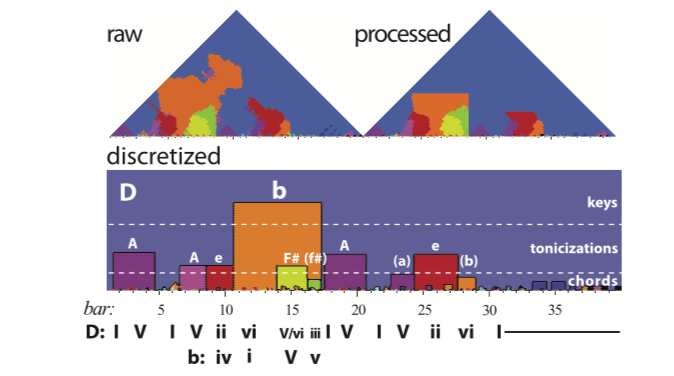
\includegraphics[width=0.7\textwidth]{figures/Q5_1.png}
%     \caption{Visualization of the difference between a
%     modulation and a tonicization, according to Sapp
%     \parencite{sapp2011computational}. The horizontal
%     lines in the bottom plot delimit a tonicization from a
%     modulation} \label{fig:Q5_1} \end{figure}

Finally, Sapp discussed the possible overlap of the terms
modulation and tonicization in music theory and proposes
that the difference between a modulation and a tonicization
can be observed in his \emph{keyscape} diagrams
\parencite{sapp2011computational}. This visualization can be
seen in Figure \ref{fig:Q5_1}, the dotted horizontal lines
\emph{separate} one concept from another. In the paper, Sapp
did not include any evaluation that compared whether the
annotations from an expert theorist would match the
divisions in his \emph{keyscapes} figures. Yet, this is
probably the only---quantitative and
computationally-applicable---proposal for distinguishing a
modulation from a tonicization.


\guide{The terminology in music theory}

In traditional music theory, the terms \emph{local key} and
\emph{global key} are virtually non-existent. The issues of
ambiguity concern mostly the distinction between
tonicization, modulation, and applied dominants.

Regarding this, Kostka and Payne write in their book
\parencite{kostka2018tonal}: \emph{The line between
modulation and tonicization (using secondary functions--V/V
and so on) is not clearly defined in tonal music, nor is it
meant to be. One listener might find that a very short
passage tonicizing a new tonality is enough to make a
convincing modulation}.

Holtmeier writes about Hauptmann’s theory and the emergence
of applied dominants as a terminology
\parencite{gollin2012reception}: \emph{In the eyes of its
supporters, function theory was predestined ``to demonstrate
how superficial are judgments that assert: `Wagner is always
modulating!' '' Applied dominants and Hauptmann's concept of
the "major-minor key“ allow the theory of functions to
interpret harmonically rich progressions within one key
without having to invoke modulations. The idea of the
applied dominant was the necessary harmonic linking module,
so to speak, within a conception of tonality that had
distanced itself from a narrow diatonic notion of
relations.}

Tchaikovsky does not talk about tonicization
\parencite{tchaikovsky2005guide}, instead, discusses
\emph{transient modulations}. Transient modulations are
modulations in which several keys are reached first,
temporarily, before arriving to the final key destination.

% \begin{figure}[h] \centering
%     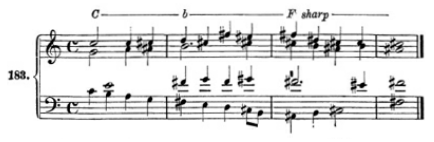
\includegraphics[width=0.7\textwidth]{figures/Q6_2.png}
%     \caption{Example of a \emph{transient modulation} as
%     it appears in Tchaikovsky's manual of harmony.}
%     \label{fig:Q6_2} \end{figure}

For Rameau \parencite{rameau1971treatise}, the concept of a
modulation, rather than a change of key, seems to refer to a
key region (similar to what Izmirli and Papadopoulos would
consider a local key). This is most clear in his seventh
rule for passing from one key to another: \emph{After having
passed through several other keys, we must modulate in this
principal key for a little longer towards the end than at
the beginning.} The fact that one may ``modulate for a
little longer'' in a given key, is an uncommon idea in later
music theories. In this sense, Rameau's modulation is, in
some way, more compatible with modern local key-finding
algorithms.





% \guide{What is a modulation?}

% A shift between a previously established key and a new
% perceived key A change in the distribution of pitch
% classes of the current scale A perfect authentic cadence
% in a different key than the main key(?)


% \guide{What is a tonicization?} A sudden reinterpretation
% of the tonal context for a specific chord or short chord
% sequence A deceptive modulation, which abruptly comes back
% to the original key A modulation that happens on a local
% scale, without major implications on the length of a piece
% The term tonicization was introduced later in music
% history, mostly to distinguish meaningless modulations
% from “real” modulations



% \guide{Differentiating a modulation from a tonicization}
% Most people who study these concepts quantitatively agrees
% that these concepts differ only in their scale, but
% represent the same phenomenon People who disagree with the
% two concepts being different only in their length will
% typically do it on the basis of structural constraints (or
% rules) that apply to modulations for being modulations and
% do not apply to tonicizations This sort of disagreement
% lies within what Temperley calls the “distributional” and
% “structural” views of computational music analysis


% \guide{Dealing with keys in computational studies}

% Computationally, researchers have usually characterized
% this phenomenon (different musical keys within a piece)
% with the umbrella term, local keys, which differs with the
% key of the entire piece, that is, the global key Local
% keys refer to keys within a sequence of music Global keys
% refer to the principal (or main, or first and last key) of
% a sequence of music This is also problematic and
% controversial


%  \guide{On the unambiguous determination of local and
% global keys} Whether we are referring to a symbolic or
% audio representation of music, musical inputs such as the
% ones received by a key-finding algorithm are typically
% sequential.

% In symbolic representations, the units of the input
% sequences can take the form of individual notes, onset
% slices with one or more notes, measures, pitch-class
% vectors, or other units.

% In audio representations, the units of the input sequences
% usually take the form of samples of a waveform or a
% spectral representation.

% If we want to differentiate the terms local and global
% key, one way of doing it is by providing a \emph{local}
% key label for each element of the sequence that is
% received by the algorithm. For example, if the symbolic
% music file received by a key-finding algorithm consists of
% 4,000 notes, the local keys could consist of 4,000 key
% labels, associated with each of the notes in the input,
% and a global key that explains the overall key of the
% 4,000 notes.

% In the image domain, this is a very common procedure known
% as image segmentation. In image segmentation tasks,
% usually one class is assigned to every pixel in the image.
% This ensures that

% A sequence of music is a sequence of musical input nodes
% If we talk about symbolic: the sequence is a sequence of
% notes and rest symbols IF we talk about audio: The
% sequence is a sequence of audio frames and their FFT
% output How long is that sequence? As long as it is
% relevant for a particular analysis A local key is a key
% that explains the key of the minimum node of that sequence
% A global key is a key that explains the key of the
% sequence itself



% \guide{The length of a piece} Easiest solution, describes
% a single movement Single movements are not always
% explained by a single key This issue can suffer of similar
% contradictions as modulations/tonicizations

    \phdsubsection{automatic chord recognition}
    \phdsubsection{multitask tonal analysis}
        \phdsubsubsection{on pitch spelling}
            % Taken verbatim from comps Q7

% A pitch-spelling algorithm is an algorithm that attempts
% to recreate the original spelling of a pitch-class in the
% context of a musical composition.

% This is a common problem in MIDI representations, as MIDI
% representations \emph{drop} all the spelling information
% of a note, leaving only the pitch class and octave.

% However, this is not an exclusive problem associated with
% MIDI representations, it would also happen when we observe
% the performance of a piece in a piano keyboard, we do not
% explicitly know whether the key played by the performer
% was intended to be an F\# or a Gb.

% Different approaches have been attempted to reconstruct
% the original spelling of a musical score.

% One of the advantages of pitch-spelling as a computational
% problem, is that it is much easier to evaluate than other
% musical problems like key classification or chord
% recognition, as it presents less ambiguity.

% \guide{Meredith}



% Meredith and Wiggins suggest that pitch-spelling
% algorithms can be used to improve the performance of
% key-finding algorithms.

% The study of Meredith and Wiggins is limited to music from
% the baroque and classical period. As of now, there are
% high-quality corpora of 19th century romantic music that
% could be integrated in a similar study.

% Meredith and Wiggins suggest that until no reliable
% pitch-spelling algorithm exists, it is theoretically
% impossible to reconstruct a notated score if given only a
% MIDI file as input.

% According to Meredith and Wiggins, knowing the spelling of
% a name also facilitates certain type of musical queries,
% for example, looking for a sequence of diatonic intervals.
% Without the knowledge of the spelling, these type of
% queries can only be approximated, and according to their
% research, they are also slower than looking for an exact
% match.

% In the study by Meredith and Wiggins, the evaluation
% metric is the raw proportion of note names that have been
% correctly spelled from the total number of spellings in
% the dataset. It is important to remark that the spellings
% of notes are not evenly distributed, particularly for
% diatonic degrees of the C Major scale (i.e., white keys in
% a piano keyboard). That is, an algorithm that predicts the
% pitch-class 0 as C would be correct most of the times, as
% it is rarely spelled as B\# or Dbb. In machine learning
% classification experiments, this problem is usually
% addressed by using different metrics of evaluation that
% account for a sparse distribution of the classes in the
% dataset. The problem of pitch-spelling requires,
% therefore, an improved method of evaluation that provides
% more meaningful information than the raw number of notes
% that have been correctly spelled.

% A derivate issue of pitch spelling algorithms is---what I
% denote---an accidental overflow. When the tonal changes in
% a score lead to a key that requires an exhaustive use of
% accidentals (e.g., double flats, or double sharps),
% composers will likely move the spellings to have less
% accidentals, for example, by notating the music in an
% enharmonic key instead.

% Meredith and Wiggins discuss one instance of such
% accidental overflow that they found in their dataset,
% Haydn's Symphony No. 100 in G Major ('Military'), in which
% a sudden change of pitch spellings implies that the piece
% moved from Db Major to C# Major, although the only
% motivation of this change of spelling is to simplify the
% notation.

% Meredith and Wiggins address this issue in their
% evaluation by providing alternative assessments of that
% fragment of music, that is, if an algorithm decided to
% spell the entire section as either C# Major, Db Major, or
% change it midways, they should all be considered correct
% to a certain extent. This, of course, is one instance of
% such issue but it needs to be addressed more formally in
% future evaluations.

% Meredith and Wiggins provide a review of 5 pitch-spelling
% algorithms (plus several variations of those algorithms):
% Longuet-Higgins, Cambouropoulos, Temperley and Sleator,
% Chew and Chen, and Meredith.

% In the evaluation from Meredith and Wiggins, the inclusion
% of sections with accidental overflow reduced the accuracy
% score of the algorithms, particularly, Temperley and
% Sleator, to the point that this section was removed from
% the evaluation.

% \guide{teodoru and raphael} Teodoru and Raphael presented
% a pitch-spelling algorithm that was tested using the same
% dataset used previously by Meredith. Their algorithm
% performs favorably compared to the other known
% pitch-spelling algorithms.

% Teodoru and Raphael note the necessity of a reliable
% pitch-spelling algorithm, particularly for the use within
% music notation software. They note: "[...] at present, the
% pitch-spellings from the commercial music notation
% programs we know of leave much to be desired". It is worth
% mentioning that over a decade has passed since this paper
% was published and researching the current state of
% pitch-spelling algorithms implemented in commercial music
% notation software could show substantial improvement
% today.

% Teodoru and Raphael tackle the problem by assuming that
% the spelling of a note can be explained through analyzing
% voice leading and local harmony.

% Teodoru and Raphael collect principles and guidelines for
% spelling notes from music theory textbooks, and try to
% incorporate such principles in the design of their
% algorithm. An example of those principles is taken from
% Aldwell's book: "avoiding “remote” accidentals; thus B♭ is
% preferred to A♯ in C major, since the former is in the
% scale of the F major, which is near to C.".

% It could be understood from such principles that there is
% an "optimal" spelling. Considering that the objective of
% spelling is to reduce the number of accidentals to the
% minimum, every spelling that is closer to C Major is
% therefore simpler, as it requires less accidentals in its
% spelling.

% Teodoru and Raphael claim that their algorithm produces an
% error that is lower than the best of Meredith's algorithms
% by a factor of more than 3.

% The model from Teodoru and Raphael assumes that the music
% will be provided as individual voices, which is a
% reasonable assumption for inputs that imply a separation
% of individual voices (i.e., chorales), but becomes a huge
% limitation for other keyboard music and other types of
% music where this separation is not provided and not
% obvious.

% Teodoru and Raphael claim that estimating the time-varying
% key (local key) is the most important element for pitch
% spelling. Additionally, they consider that the
% relationship between local keys and spelling is
% bidirectional, that is, spelling can help influence the
% choice of key as much as the key can influence the choice
% of spelling.

% Teodoru and Raphael replicate a study using the dataset
% derived by Meredith, however, the evaluation score is
% presented as an error rate, which consists in the number
% of misspelled notes divided by the total number of notes.
% They computed the error rate overall as well as for each
% of the composers in the dataset.

% Teodoru and Raphael describe that a subset of the corpus
% was used as "training data". The training data consisted
% of all of the Beethoven scores, 5 string quartet movements
% from Haydn, and a concerto movement from Mozart. This, of
% course, means that the performance shown in the paper does
% not contemplate the performance of the algorithm in a set
% of previously unseen data.

% Teodoru and Raphael report that their algorithm was
% particularly unable to correctly spell the pitches during
% harmonic progressions that involved German Augmented Sixth
% Chords, Diminished Seventh chords and other harmonic
% circumstances. They note: "Other situations require a
% deeper notion of the harmonic state than provided by the
% local key, as in the German augmented sixth chord, which
% seems nearly impossible to spell correctly without
% recognizing it as such." It may be possible that spelling
% the notes requires not only to model the interaction
% between keys and spelling but also of chords.

A pitch-spelling model is an algorithm that predicts the
original spelling that a note had in a musical score when
only the pitch-class, octave, and duration of the note are
provided as inputs to the model.\footnote{Some researchers
have also found helpful to know the voice (\emph{stream}, in
psychoacoustics) in which the note is sounding. However,
this information departs from what can be reliably obtained
from real-world digital music files. Therefore, a real-world
algorithm should work regardless of whether it knows what
voice played the note.}

To understand the problems that derive from pitch-spelling,
the following example could be considered. If during a
musical performance, a pianist presses the key corresponding
to the pitch class number 8 in the piano keyboard (shown in
Figure  \ref{fig:Q7_1}), how can we know if the note played
by the performer was an A$\flat$ or a
G$\sharp$?\footnote{Assume an equal-tempered setting, with
no special considerations regarding how the piano might be
tuned. That is, the distinction between the A$\flat$ and
G$\sharp$ notes that we are looking for is of a semantic
nature.}

% \begin{figure}[h] \centering
%     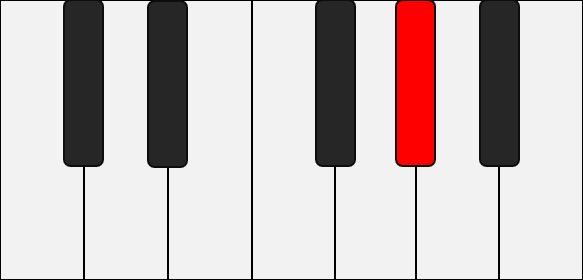
\includegraphics[width=0.6\textwidth]{figures/Q7_1.png}
%     \caption{A note playing in a keyboard. It could be
%     either G$\sharp$ or A$\flat$.} \label{fig:Q7_1}
%     \end{figure}

This example problem may seem ingenuous at first, however,
the spelling of a note could \emph{carry} much more
information about the tonal context of the music that one
might expect. Similarly, the reverse problem (spelling the
note) may \emph{require} much more information about the
tonal context of the music that one might expect. This
double relationship between the acquired and delivered
musical knowledge in the spelling of a note is what makes it
an interesting computational problem, as it provides a
framework for assessing quantitatively the extent to which a
computational model understands the musical semantics.
Furthermore, finding the spelling of a note has the
additional advantage of being highly unambiguous as an
evaluation metric compared to other analytical tasks like
finding the musical key \parencite{gebhardt2018confidence}
or labeling the chords in a piece
\parencite{ni2013understanding}.

In order to better contextualize what is the information
contained in the spelling of a pitch, let us extend the
previous thought exercise a bit further.

A first impulse that someone might have for guessing whether
the note is A$\flat$ or G$\sharp$ could be to know the
musical key of the piece during which the piano key was
played. Such information can be obtained from a key-finding
model and there are many approaches that could provide it
with a reasonable degree of accuracy. Nevertheless, our
pitch-spelling model now requires information about the key
in order to make its predictions.

It could be assumed that the model will receive such
predictions, and that they are reliable. A key-finding model
could then inform us that the piece was in \emph{A minor}.
``Is it a piece in A minor?'' Then the note is probably a
G$\sharp$.

% \begin{figure}[h] \centering
%     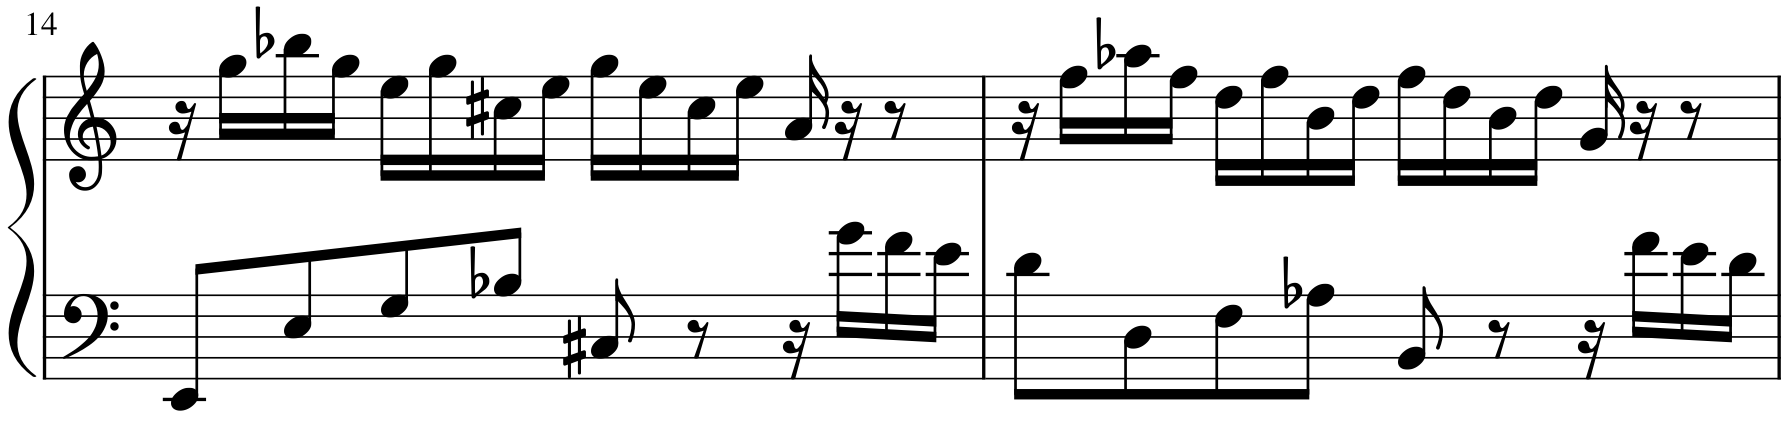
\includegraphics[width=0.8\textwidth]{figures/Q7_2.png}
%     \caption{J. S. Bach's BWV 784, mm. 14-15. The piece is
%     in A minor, however, during measure 15, the pitch
%     class number 8 is spelled as an A$\flat$.}
%     \label{fig:Q7_2} \end{figure}

Figure \ref{fig:Q7_2} shows an adversarial example where the
pitch class number 8 is spelled as A$\flat$ in a piece that
is originally in \emph{A minor}. A person familiarized with
Western tonal music could guess that similar examples as the
one shown in Figure \ref{fig:Q7_2} will occur whenever the
music is modulating or tonicizing a different key.

Assuming that the awareness of modulations and tonicizations
throughout the piece (which we generally refer to as
\emph{local keys}) will mitigate our problems when
predicting the spelling of a note, seems to be a reasonable
guess. Instead of requiring to know the \emph{global key} of
the piece, now, our model requires to know the \emph{local
keys} throughout the piece. Notice, however, that there are
much less models available that provide such information,
and that there is no sufficient amount of research assessing
whether they are accurate or not, mostly because the
concepts of modulation and tonicization are problematic and
ambiguous themselves (see Question \ref{chap:chap6} for a
further discussion on modulation and tonicization).

To complicate the matter a bit further, there are other
circumstances that affect the spelling of a note, such as
the use of non-chord tones or the harmonic context. One
example of the implications of non-chord tones is, as shown
in Figure \ref{fig:Q7_3}, the spelling of a chromatic
neighbouring note, which should probably have a different
note name than the \emph{real} note.

% \begin{figure}[h] \centering
%     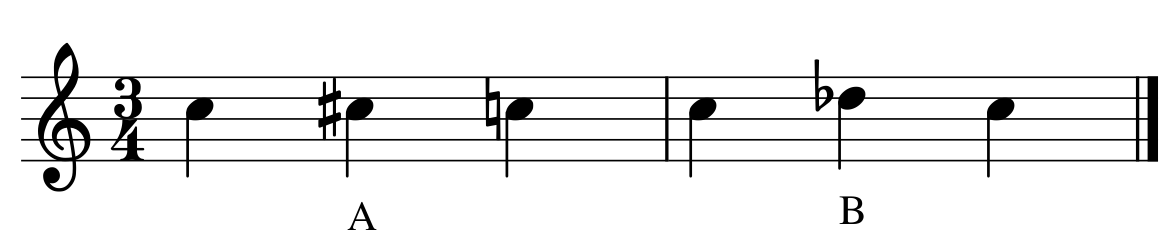
\includegraphics[width=0.8\textwidth]{figures/Q7_3.png}
%     \caption{Two notations (A and B) of a chromatic
%     neighbouring note. Regardless of the harmonic and key
%     context, the second note should probably be spelled as
%     in version B.} \label{fig:Q7_3} \end{figure}

One example of a complicated harmonic context is the
presence of a German augmented sixth, for which Teodoru and
Raphael write \parencite{teodoru2007pitch}: \emph{Other
situations require a deeper notion of the harmonic state
than provided by the local key, as in the German augmented
sixth chord, which seems nearly impossible to spell
correctly without recognizing it as such.}

Overall, designing a pitch-spelling algorithm poses
important challenges in different musical fronts, but it
also provides researchers with the opportunity of putting in
practice different analytical models (e.g., local key, chord
labeling, and non-chord detection) for solving a common
task. Furthermore, unlike many of those models which suffer
from highly ambiguous evaluations, pitch spelling presents a
simple way of assessing whether our computational models
understand the musical context or not. That is, the note is
either G$\sharp$ or A$\flat$, and there is only one right
answer.

In the following section, a survey is provided with
different pitch-spelling algorithms that have been developed
throughout the years.

\guide{A brief survey of pitch-spelling algorithms}

Compared to other tasks of Music Information Retrieval
(MIR), there have not been as many attempts to solve the
problem of pitch spelling. Nevertheless, it is likely that
there are other solutions to the problem, in commercial
applications, which are not described in the literature and
in this survey. This is due to the fact that pitch-spelling
is a highly relevant problem for commercial software that
deals with the conversion of MIDI files into music scores,
for example, most music notation editors.

% \guide{Longuet-Higgins (1976)}
In 1976, Longuet-Higgins presented what is arguably the
first pitch-spelling algorithm
\parencite{longuethiggins1976perception}. It is limited to
work on monophonic melodies. Longuet-Higgins considered that
any note could be assigned a number, $p$, based on
3-variables that related the note with respect to
\emph{middle C}: the distance in perfect fifths, the
distance in major thirds, and the octave. Using that
methodology, Longuet-Higgins extended the notation to add a
``sharpness'' feature, $q$, which was defined based on the
distance in fifths and thirds to \emph{middle C}, irrelevant
of the octave. This ``sharpness'' value, in conjunction with
the MIDI note number, was used to indicate the spelling of
the note.

% \guide{Cambouropoulos (2003)}
After a gap of around 25 years, a series of new algorithms
were developed by different researchers independently,
almost at the same time. In 2003, Cambouropoulos presents an
approach that heavily relies in intervals
\parencite{cambouropoulos2003pitch}. The algorithm uses a
shifting overlapping window (suggested to be of 9 to 12
pitches long). The window moves along the sequence of
pitches, from left to right, until the sequence concludes.
For each window, the pitch-spelling process optimizes two
aspects: 1) that notes make the minimum use of accidentals
(something that Cambouropoulos refers to as \emph{notational
parsimony}), and 2) the avoidance of 8 classes of augmented
and diminished intervals (something that Cambouropoulos
refers as \emph{interval optimization}). The algorithm was
evaluated on Mozart piano sonatas and Chopin Waltzes.

% \guide{Chew and Chen (2003)}
After its introduction in her dissertation, the Spiral Array
model by Chew was used for multiple tasks that involved
tonal analysis, for example, chord labeling, key-finding,
and pitch-spelling \parencite{chew2000towards}. The Spiral
Array is a spatial representation of tonality that allows a
sequence of pitches to be \emph{positioned} in
the---theoretical---tonal space, which facilitates the
computation of tonal features in different ways. Regarding
the pitch-spelling problem, three different algorithms were
proposed by Chew and Chen \parencite{chew2003determining}
that were built on top of each other. In the paper, their
evaluation of the algorithms restricted to few movements of
Beethoven's piano sonatas.

% \guide{Temperley and Sleator (2004)}
Throughout the late 1990s and early 2000s, Temperley
developed a series of algorithms for modelling different
aspects of musical structure (i.e., meter, phrasing,
counterpoint, harmony, key, and pitch-spelling). These
models were implemented by Daniel Sleator in the
\emph{Melisma Music Analyzer} and explained in detail in the
book by Temperley \parencite{temperley2004cognition}.
Respecting the pitch-spelling problem, the approach by
Temperley consists of a rule-based system based on his
concepts of \emph{Tonal Pitch Class (TPC)} and the
\emph{line of fifths}. Additionally, the algorithm depends
on the metrical analysis provided by the Melisma Music
Analyzer, before extracting the spelling of the notes.

% \guide{Meredith (2003)}
Meredith introduced an algorithm that receives MIDI note
numbers and onset times as ordered pairs and determines the
spelling of the notes through 2 stages
\parencite{meredith2003pitch}. The first stage consists of a
rule-based system with 8 rules that are carried out in
sequence. After the first stage, the algorithm has
determined a spelling for the notes. The second stage,
consists of the correction of the outputs given by the first
stage. The corrections performed account for neighbouring
notes or passing notes which could have been erroneously
predicted by the first stage. In a subsequent study
\parencite{meredith2005comparing}, Meredith compared its
pitch-spelling algorithm against other pitch spelling
algorithms, determining that his algorithm had the highest
accuracy.



% \guide{Stoddard et al. (2004)}
Stoddard et al. proposed a new algorithm for pitch-spelling
\parencite{stoddard2004welltempered}. Their approach is
data-driven, which requires ground-truth spelling
information in order to be trained. Additionally, their
algorithm runs on top of a probabilistic framework of
harmonic analysis \parencite{raphael2003harmonic} and it is
conditioned by the accuracy of that harmonic analysis model.
The algorithm was evaluated over a total of 22,593 notes,
scoring 96.87\% accuracy. During their study, they found
that the detection and resolution of voice-leading
considerations (i.e., the relationship between a note and
its immediate neighbours) was the most important feature to
consider in a pitch-spelling algorithm.

% \guide{Teodoru and Raphael (2007)}
Teodoru and Raphael tackled the problem by assuming that the
spelling of a note depends on voice leading and local
harmony \parencite{teodoru2007pitch}. They observed
principles and guidelines for spelling notes from music
theory textbooks \parencite{aldwell2017harmony,
rimskykorsakov2005practical} and attempted to build a
probabilistic model that \emph{captures} these relationships
through the use of Markov chains. In their evaluation, they
showed that their model outperformed every other model,
including Meredith's \parencite{meredith_ps13_2006}.
Nevertheless, an important drawback from their approach is
that it assumes that the music will be provided as
individual voices, which is not a reasonable assumption for
real-world MIDI inputs and, therefore, limits the
application of their algorithm in practice. In their study,
they found that estimating the time-varying key (local key)
is fundamental for pitch spelling. Additionally, they
consider that the relationship between local keys and
spelling is bidirectional. That is, spelling can help
influence the choice of key as much as the key can influence
the choice of spelling.


    \phdchapter{data acquisition and preparation}

% \begin{quote} A quote \end{quote} \clearpage

\phdsection{available datasets}
    \phdsubsection{annotated beethoven corpus (ABC)}
    \phdsubsection{beethoven piano sonatas (BPS)}
    \phdsubsection{haydn ``sun'' string quartets (HaydnSun)}
    \phdsubsection{music theory examples (MuThEx)}
        \guide{Dataset}~\label{sec:dataset} All the labels in the
dataset have been obtained from the modulation excerpts of
five music theory textbooks, written by different music
theorists and/or composers (whom we simply refer to as
``theorists'' for the rest of this paper).

The dataset contains, in total, 201 excerpts of music with
annotated modulations and tonicizations. The annotations are
encoded in the form of roman numerals of all the chords in
the dataset, which can be helpful for utilizing the dataset
for other purposes beside the one presented here (e.g.,
chord labeling or cadence detection). Each file has been
encoded in Humdrum (**kern) symbolic music representations
~\cite{huron02humdrum}. As mentioned, the roman numeral
annotations have been digitally encoded
\cite{napoleslopez20harmalysis} within the scores.

When the theorists provided roman numeral annotations, those
have been preserved in our digital transcriptions.
Otherwise, we furnished them. All the annotations related to
modulations have been obtained exclusively from the
textbooks. Tonicizations rely on the roman numeral
annotations of the chords and these were not always provided
in the textbooks, therefore, we supplied some of them.

The issues of ambiguity discussed in Section
\ref{sec:ambiguity} might have implications mostly for
tonicizations (the ones we sometimes contributed ourselves).
However, modulations have always been provided by the
theorists, and we expect this to reduce the impact of these
issues. For some onsets, multiple key annotations were
provided by the theorists. For these excerpts, we decided to
encode the keys in chronological order. An example is shown
in Figure \ref{fig:multiplekeys}.\footnote{Whenever a new
key was established according to the theorists' annotations,
we considered that to be the only key in the modulation
column, until a new one appeared to replace it. We applied
this process systematically throughout the dataset.
%Despite the loss of informations, this unique annotation line is more easily processed by local key estimation models.
}

% \begin{figure}[h]
%   \centering
%   \includegraphics[width=\linewidth]{figs/multiplekey2}
%   \caption{Example 18-3 in Kostka-Payne's Tonal
%   Harmony~\cite{kostka2008tonal}. Two concurrent keys (G
%   Major and F Major) are annotated in the fourth beat of
%   measure 1. We considered the key label of this onset to be
%   ``F Major'' for the modulation column.}
%   \Description{Example 18-3 in Kostka-Payne's Tonal Harmony.
%   Two concurrent keys appear in the same onset.}
%   \label{fig:multiplekeys}
% \end{figure}

We describe the five textbooks and their abbreviations,
which we use throughout the experiment section.

\guide{Sources of the Annotations}

	\guide{Aldwell, Schachter, and Cadwallader~(ASC) [USA, contemporary]}
	The modulation excerpts are taken from chapter 27
	\emph{Diatonic Modulations} of the \emph{Harmony and
	Voice Leading} ~\cite{aldwell2018harmony}. This textbook
	provided seven excerpts to the dataset, the smallest
	amount among all textbooks. These excerpts are extracts
	from Bach Chorales (4), Mozart's Trio for Clarinet (1),
	and two original examples.

	\guide{Kostka and Payne~(KP) [USA, contemporary]}
	The modulation excerpts are taken from the 18th and 19th
	chapters of \emph{Tonal Harmony}~\cite{kostka2008tonal}.
	We took fifteen excerpts from this book, which are
	fragments of pieces written by Classical and Romantic
	composers. Previously, the annotated audio excerpts of
	the accompanying workbook were used for another
	local-key estimation study \cite{izmirli2007localized},
	however, we encoded the score excerpts of the main
	textbook.

	\guide{Reger~(Reg) [Germany, 1904]}
	A hundred modulation excerpts are taken from \emph{On
	the Theory of Modulation}\footnote{The book we used is
	the republication by \emph{Dover} with the title
	\emph{Modulation} (2007).}~\cite{regermodulation}. The
	excerpts are very short and they are all written by
	Reger himself. Reger's goal was to provide cadence-like
	examples of modulation from two keys (C major and A
	minor) to almost every other possible key.

	Seventeen of the examples had two terminations: one in a
	major key and one in a minor key.\footnote{Usually
	parallel keys that shared a closing dominant harmony and
	resolved to either the major or minor mode, with the
	same tonic.} We separated these examples into two files,
	one for each of the terminations. This increased the
	total number of examples from 100 to 117.

	\guide{Rimsky-Korsakov~(Rim) [Russia, 1886]}
	The modulation excerpts are taken from the third section
	of the \emph{Practical Manual of
	Harmony}~\cite{rimskitonality}. As with Reger, all the
	thirty-seven examples in this textbook are written by
	the author himself. Some of the examples, however, are
	more detailed and longer in duration than the ones by
	Reger.

	\guide{Tchaikovsky~(Tch) [Russia, 1872]}
	The modulation examples considered are taken from the
	third section of the \emph{Guide to the Practical Study
	of Harmony}~\cite{tchaikovsky1872guide}. All twenty-five
	examples were written by Tchaikovsky himself.

\guide{Statistics About the Dataset}\label{ssec:stats}

Some statistics about the dataset are presented in
Table~\ref{tab:dataset}. We report, for each of the
textbooks: the number of files (excerpts), the number of
modulations, the number of tonicizations, and the number of
labels (which is equivalent to the number of onsets, as we
supplied one label per onset).

% \begin{table}
%   \caption{Summary of the dataset. Each value indicates the number of occurrences in the corresponding textbook.}
% % The column ``Tonicized'' denotes the number of labels with
% % a tonicization label that differs from the key of the
% % modulation (e.g., Offset 2 in Table
% % \ref{tab:annotations}).
%   \label{tab:dataset}
%   \begin{tabular}{l|cccc}
%     \toprule
%     Sample & Files & Modulations & Tonicizations & Labels\\
%     \midrule
%     ASC & 7 & 8 & 7 & 185\\
%     KP & 15 & 21 & 11 & 554\\
%     Reg & 117 & 220 & 40 & 768\\
%     Rim & 37 & 44 & 107 & 257\\
%     Tch & 25 & 60 & 38 & 238\\
%     Total & 201 & 555 & 203 & 2002 \\
%   \bottomrule
% \end{tabular}
% \end{table}

The \emph{Reg} textbook is by far the one that contributed
the largest number of excerpts. However, the ones providing
a higher ratio of labels per number of files are \emph{ASC}
($26.42$) and \emph{KP} ($36.93$). This may be due to the
use of musical examples taken from the literature, where
modulations occur within a musical context and, therefore,
span longer regions.

\emph{Rim} and \emph{Tch} are the textbooks that provided
the highest number of tonicizations. They show tonicizations
in $41.63\%$ and $15.97\%$ of the onsets, respectively. In
terms of investigating the relationship between predicted
local keys and modulations/tonicizations, these textbooks
contributed the most interesting examples.

\emph{Rim} and \emph{Tch} also tend to set the annotations
of the \emph{destination} key of a modulation in the tonic
degree, considering any preceding dominant chords as
secondary dominants and, consequently, part of the
\emph{departure} key (as shown on Figure~\ref{fig:example}).
Other theorists, on the other hand, often set the
\emph{destination} key already in the dominant chords that
precede the tonic. Therefore, they do not annotate (or
imply)\footnote{For the cases in which we provided the roman
numeral annotations because they were not provided by the
theorists.} a tonicization for the preceding dominant
chords.

    \phdsubsection{mozart piano sonatas (MPS)}
    \phdsubsection{theme and variation encodings with roman numerals (TAVERN)}
    \phdsubsection{schubert winterreise (SW)}
\phdsection{data preparation}
    \phdsubsection{encoding issues}
        % Taken verbatim from Encoding Matters

We introduce a series of examples in which different encodings effectively modify the content of two---apparently equivalent---symbolic music files. These examples have been obtained from comparing three different encodings of a string quartet movement by Ludwig van Beethoven.

We present two scenarios in which encoding discrepancies may be introduced. In the first scenario, they have been introduced during the encoding of the symbolic music file by either the music notation software or the human encoder. The discrepancies introduced in this scenario are typically difficult to notice because they are \emph{visually} identical to an accurate encoding. In the second scenario, the discrepancies have been introduced during the translation of the original file into other symbolic formats. In this scenario, the discrepancies may be related to propagating errors in the original encoding or to an erroneous translation of certain attributes of the musical content. Finally, we discuss the possibility of using the examples provided here for the mitigation of some of these discrepancies in the future.

\guide{From conclusions}

In this paper, we have presented examples of discrepancies in symbolic music files that were encoded by different human encoders and music notation software. We also investigated the discrepancies introduced when these files were translated into other symbolic music formats. Several of the discrepancies repeat systematically in the form of patterns (e.g., users place a \emph{slur} between two notes of the same pitch when they meant to place a \emph{tie} or incomplete measures are interpreted differently in distinct music notation software).

In many cases, developing better methodologies for symbolic music corpora creation \cite{mckay2018} should set the basis for reliable data and reproducible research, however, whenever this is not sufficient, detecting the patterns leading to discrepancies---as the ones described here---seems to be a promising and worthy effort in the comparison, evaluation, and, possibly, the auto-correction of symbolic music files, which is in the interest of music researchers and digital music libraries.

        % Taken verbatim from experiment in napoleslopez2020local

\guide{Experiment}~\label{sec:exp}

In our experiment, we investigate whether the predictions of
three local-key-estimation computational models coincide
with the modulation and tonicization annotations of the
music theory textbooks.

\guide{Evaluation Procedure}~\label{sec:evaluations}

Even if two predicted keys do not match the ground-truth
label, one of the predictions may still be better than the
other, due to the \emph{close} or \emph{far} relationship
that a predicted key may have to the ground truth. For this
reason, in addition to accuracy, we propose to also use a
weighted score to evaluate each onset's key.

Table \ref{tab:mirexscore} shows the two sets of weights we
utilized to evaluate the key predictions, based on the
relationship that the predicted key has to the ground truth.
The MIREX score has been used in the annual Music
Information Retrieval Evaluation eXchange (MIREX) evaluation
of global-key-estimation algorithms since 2005
\parencite{downie2005}.

% \begin{table}[h] \begin{tabular}{l|l} \textbf{Key
% prediction's relation to the ground truth} &
% \textbf{Score} \\ \hline Same key & 1.0 \\
% Dominant / SubDominant & 0.5 \\
% Relative Major / Relative Minor & 0.3 \\
% Parallel Major / Parallel Minor & 0.2 \\
% Other & 0.0 \\
% \end{tabular} \caption{MIREX weighted score for key
% predictions.} \label{tab:mirexscore} \end{table}

% \begin{table}[h]
%     \caption{Evaluation weights for the key predictions.}
%     \label{tab:mirexscore}
%     \begin{tabular}{l|cc}
%         \toprule
%         Key Relationship (Reference, Predicted) & Accuracy &
%         MIREX \\
%         \midrule
%         Same key                                & 1.0      &
%         1.0   \\
%         Dominant / SubDominant                  & 0.0      &
%         0.5   \\
%         Relative Major / Relative Minor         & 0.0      &
%         0.3   \\
%         Parallel Major / Parallel Minor         & 0.0      &
%         0.2   \\
%         Other                                   & 0.0      &
%         0.0   \\
%         \bottomrule
%     \end{tabular}
% \end{table}

We apply both evaluations to the key of every onset in the
score. The annotations are evaluated according to Equation
\ref{eqn:mirex}.

\begin{equation}
    \label{eqn:mirex}
    \mathit{score} = \frac{\sum_{i=0}^{N} \mathit{w(k_i, l_i) d_i}}{\sum_{i=0}^{N} d_i}
\end{equation}

$N$ represents the number of onsets in the input score, $k$
is a vector of ground-truth key annotations for each onset,
$l$ is the vector of local-key predictions provided by the
model for each onset, and $d$ is a vector with the durations
in quarter notes of every onset. Note that the vector $k$
corresponds to either the labels in the \emph{Modulation} or
\emph{Tonicization} columns of Table \ref{tab:annotations},
depending on the task.

The $w$ function is a piece-wise function that evaluates
either of the weighted scores shown in Table
\ref{tab:mirexscore}, given a ground-truth key and a
prediction. The scalar value $score$ is in the range $[0,
1]$. A value of $1.0$ is obtained if and only if the model
predicts the key correctly at every onset. A value of $0.0$
is obtained if and only if the model makes incorrect
predictions (and for the MIREX weights, also without any
partial value) at each onset.

Using this methodology, we evaluate four baseline models and
three local-key-estimation models from the literature. In
total, we perform four evaluations for each model:
% (1) modulation with the accuracy weights, (2) tonicization
% with the accuracy weights, (3) modulation with the MIREX
% weights, and (4) tonicization with the MIREX weights.
\begin{enumerate}
    \item Modulation ($k=Modulation$) by accuracy
    ($w=Accuracy$).
    \item Tonicization ($k=Tonicization$) by accuracy
    ($w=Accuracy$).
    \item Modulation ($k=Modulation$) by MIREX ($w=MIREX$).
    \item Tonicization ($k=Tonicization$) by MIREX
    ($w=MIREX$).
\end{enumerate}

These evaluations coincide with the results shown in
Figure~\ref{fig:plot}.

% \begin{table}[h] \caption{Evaluations}
%  \label{tab:evaluations} \begin{tabular}{l|ll} \toprule &
%  Accuracy weights & MIREX weights \\
%     \midrule Modulation Ground Truth & Evaluation 1 &
%     Evaluation 3 \\
%     Tonicization Ground Truth & Evaluation 2 & Evaluation
%     4 \\
%  \bottomrule \end{tabular} \end{table}

\guide{Baseline Models}

We describe two baseline models (\emph{B1} and \emph{B2})
that---we expect---will perform worse than existing
local-key-estimation algorithms. Similarly, we propose two
theoretical ``models'' that set the maximum performance that
can be achieved when designing a modulation or tonicization
model (\emph{B3} and \emph{B4}). These artificial models
consist simply of the ground truth annotations for
modulations and tonicizations, but evaluated in the opposite
task (i.e., as if they were local-key predictions coming
from a model). We expect that these baselines will set a
reasonable frame for inspecting the performance of the
\emph{real} local-key-estimation models.

\guide{Random guess (B1)}
This model randomly chooses a key label for every onset in
the piece.\footnote{
    %In all of our evaluations, we collapse two enharmonic
    %spellings of a key as the same key label (in the range
    %[0--23]).
    The key label is generated by choosing randomly between
    24 possible keys ([0--23]), collapsing all enharmonic
    spellings into the same class. This may occlude
    important hints given in the note spellings of music
    scores, however it guarantees that this method can be
    applied to MIDI and audio files, which lack
    pitch-spelling information.} We expect this model
    (\emph{B1}) to be the worst-performing model in our
    experiment.

\guide{Global-key guess (B2)}
Given the large body of work that exists in
global-key-estimation algorithms, it would be reasonable to
assume that using the predictions of a global-key-estimation
model in every onset would deliver reasonable results. We
incorporate these global-key predictions as a baseline
model, to compare it against the more specialized
local-key-estimation models. The global-key-estimation model
that we considered is the default key-estimation model in
music21 \parencite{cuthbert2010music21}.

\guide{Modulation (B3) and tonicization (B4) ground truth}

Due to the overlap that exists between the modulation and
tonicization key labels,\footnote{This is because we
duplicate the modulation label in the tonicization column
unless there is a tonicization (see Table
\ref{tab:annotations}).} it is expected that a
good-performing modulation model would also achieve a good
performance in predicting tonicizations (and vice versa). In
order to observe this, we consider two additional models:
the ground truth of modulation employed as a ``model'' that
predicts tonicization (\emph{B3}), and the ground truth of
tonicization employed as a ``model'' that predicts
modulation (\emph{B4}). For simplicity, we refer to these as
baseline models, although they represent ground-truth
annotations and not computational models per se.

We evaluate the performance that each of these theoretical
models, \emph{B3} and \emph{B4}, achieves in its own task
and the opposite one. More specifically, we expect the
following: (1) these models should obtain a perfect score in
their own task (no matter which weights are utilized) and
(2) both models should obtain an identical performance when
evaluated in the opposite task.\footnote{This is also true
for the MIREX weights, because the evaluation is
symmetrical. That is, $w(gt, pred) = w(pred, gt)$; when
$w=MIREX$}

\guide{Local-Key Models from the Literature}
Three recent models of local-key estimation are evaluated.
As part of the results in this paper, we intend to
investigate whether these three models are better suited for
finding ``modulations'' or ``tonicizations''. We consider
that this methodology could equally be applied to other
symbolic and audio local-key-estimation models.

\guide{N\'{a}poles L\'opez et al. (M1)} This model computes
two stages of output: local keys and a global key
\parencite{napoleslopez2019key}. Both stages are computed through
an HMM. The main parameters of the HMM are a set of
\emph{key profiles} and a table of key distances. We compute
both stages but only evaluate the local-key predictions. The
model is applied with its default parameters.

\guide{Feisthauer et al. (M2)}
This model estimates the succession of keys and can be
configured by adjusting the weights associated to three
proximity measures~\parencite{feisthauer2020smc}. Two sets of
weights are used. The first set consists of the default
weights when the model is not trained (M2a). The second set
consists of the optimal weights after training the model on
Mozart's string quartets (M2b).

\guide{Micchi et al. (M3)}
This model was introduced by Micchi et
al.~\parencite{micchi20roman} and utilizes an LSTM network to
provide the harmonic analysis of a musical excerpt, which is
described through six features: key, degree 1, degree 2,
quality, inversion, and root. We evaluate the key
predictions of the model when it is used without any
post-processing. A web application is also provided by
Micchi et al. to facilitate the process of generating these
or other
annotations.\footnote{\url{http://roman.algomus.fr/}}

All of the local-key-estimation models have been trained on
different datasets (see Table \ref{tab:corpus}) and have
been used with their default parameters. The dataset of
modulations and tonicizations introduced in Section
\ref{sec:dataset} has been utilized only as a \emph{test}
set to these models. It is likely that the models would
achieve better results if they were trained on a sample of
the dataset. However, the current size of the dataset is not
sufficient to provide training, validation, and test splits.
Therefore, we decided to limit its use as a test set. With
this, we investigate the generalization capabilities of
these pre-trained models.

\guide{Results and discussion}~\label{sec:res}

Figure \ref{fig:plot} shows the four evaluations of the
baseline and local-key-estimation models. The MIREX scores
are generally higher because they reward a key prediction
that is \emph{nearby} the correct class. This has increased
the results of virtually all models. However, the global-key
baseline model (\emph{B2}) has benefited the most from the
MIREX evaluation, followed by \emph{M2b}. This suggests that
these models predict keys that are nearby the ground truth,
while other models tend to ``hit-or-miss''.

For the reverse ground truth ``models'', \emph{B3} and
\emph{B4}, the results are symmetric, as expected. When they
are used in the opposite task, they have a quasi-perfect
evaluation on \emph{ASC}, \emph{KP} and \emph{Reg}.
Incidentally, this shows the relatively low number of
tonicizations in these textbooks (see Section
\ref{sec:tonicization}). However, in \emph{Tch} and
especially \emph{Rim}, where there is a heavier use of
tonicizations, the local-key-estimation models show an
inclination toward the tonicization predictions, rather than
the modulation ones. This is unexpected, as most researchers
do not describe their local-key-estimation models as
``tonicization finders''.

As expected, the random-guess baseline (\emph{B1}) is the
worst performing model in all evaluations. It also
highlights the success of the global-key-estimation model
(\emph{B2}) compared to a random guess. This model
(\emph{B2}) achieves good performance overall; in the
\emph{Reg} examples, it even achieves better performance
than all the specialized local-key-estimation models
(\emph{M1}, \emph{M2a-b}, and \emph{M3}).

% Despite that this dataset is specialized on musical
% contexts with modulations and tonicizations, there are
% still many onsets that match the prediction of the global
% key.

The N\'apoles L\'opez et al. model \emph{(M1)} achieves a
good performance overall, and does slightly better in
predicting tonicizations than modulations. This is at least
the case for \emph{Tch}, and more evidently, for \emph{Rim}.


% \begin{figure*}
%     \centering
%     \includegraphics[width=\linewidth]{figs/plots_table}
%     \caption{Evaluation scores for each model on each
%     textbook of our dataset. The models predict modulations
%     and tonicizations. Furthermore, they are evaluated using
%     accuracy and MIREX weights, as described in Section
%     \ref{sec:evaluations}. A plot is shown for each of the
%     four evaluations. The $y$ axis shows the evaluations on
%     different textbooks of our dataset, as the performance
%     varies from one to another. The $x$ axis shows the mean
%     score obtained by a model across all the files in the
%     textbook. Bold scores indicate the best-performing model
%     in a given textbook and task, excluding \emph{B3} and
%     \emph{B4} (see Section 4.2.3).}
%     \label{fig:plot}
%     \Description{A plot of the results for both tasks
%     according to the MIREX score.}
% \end{figure*}

% \begin{table} \caption{Accuracy score.}
%  \label{tab:acc_results} \begin{tabular}{clccccc} \toprule
%  Model & Task & ASC & KP & Reg & Rim & Tch\\
%     \midrule B1 & Mod & 0.05 & 0.03 & 0.02 & 0.04 & 0.03\\
%       & Ton & 0.05 & 0.03 & 0.02 & 0.07 & 0.05\\
%     B2 & Mod & 0.61 & 0.49 & \textbf{0.53} & 0.28 & 0.25\\
%       & Ton & 0.62 & 0.48 & \textbf{0.52} & 0.52 & 0.34\\
%     \hline M1 & Mod & 0.82 & 0.74 & 0.45 & 0.35 & 0.51\\
%       & Ton & \textbf{0.84} & 0.75 & 0.45 & 0.69 & 0.63\\
%     M2a & Mod & 0.78 & 0.52 & 0.36 & 0.35 &
%     \textbf{0.70}\\
%         & Ton & 0.79 & 0.52 & 0.36 & 0.47 &
%         \textbf{0.77}\\
%     M2b & Mod & 0.44 & 0.39 & 0.11 & 0.37 & 0.41\\
%         & Ton & 0.44 & 0.39 & 0.11 & 0.27 & 0.32\\
%     M3 & Mod & \textbf{0.83} & \textbf{0.83} & 0.48 &
%     \textbf{0.40} & 0.58\\
%       & Ton & 0.83 & \textbf{0.83} & 0.49 & \textbf{0.75}
%       & 0.72\\
%     \hline B3 & Mod & 1.00 & 1.00 & 1.00 & 1.00 & 1.00\\
%       & Ton & 0.98 & 0.98 & 0.97 & 0.57 & 0.78\\
%     B4 & Mod & 0.98 & 0.98 & 0.97 & 0.57 & 0.78\\
%       & Ton & 1.00 & 1.00 & 1.00 & 1.00 & 1.00\\
%  \bottomrule \end{tabular} \end{table}

% \begin{table} \caption{MIREX weighted score}
%  \label{tab:mirex_results} \begin{tabular}{clccccc}
%  \toprule Model & Task & ASC & KP & Reg & Rim & Tch\\
%     \midrule B1 & Mod & 0.09 & 0.10 & 0.08 & 0.11 & 0.10\\
%       & Ton & 0.10 & 0.10 & 0.08 & 0.13 & 0.13\\
%     B2 & Mod & 0.69 & 0.60 & \textbf{0.58} & 0.46 & 0.37\\
%       & Ton & 0.69 & 0.59 & \textbf{0.57} & 0.64 & 0.47\\
%     \hline M1 & Mod & \textbf{0.86} & 0.83 & 0.53 & 0.49 &
%     0.61\\
%       & Ton & \textbf{0.87} & 0.83 & 0.54 & 0.77 & 0.74\\
%     M2a & Mod & 0.84 & 0.58 & 0.45 & 0.51 &
%     \textbf{0.75}\\
%         & Ton & 0.84 & 0.58 & 0.45 & 0.58 &
%         \textbf{0.81}\\
%     M2b & Mod & 0.63 & 0.47 & 0.18 & \textbf{0.55} &
%     0.49\\
%         & Ton & 0.63 & 0.46 & 0.18 & 0.43 & 0.41\\
%     M3 & Mod & \textbf{0.86} & \textbf{0.88} & 0.55 & 0.53
%     & 0.67\\
%       & Ton & 0.86 & \textbf{0.88} & 0.56 & \textbf{ing} &
%       0.80\\
%     \hline B3 & Mod & 1.00 & 1.00 & 1.00 & 1.00 & 1.00\\
%       & Ton & 0.99 & 0.98 & 0.98 & 0.65 & 0.81\\
%     B4 & Mod & 0.99 & 0.98 & 0.98 & 0.65 & 0.81\\
%       & Ton & 1.00 & 1.00 & 1.00 & 1.00 & 1.00\\
%  \bottomrule \end{tabular} \end{table}

The proximity measure model \emph{M2a} gets a lower average
score than \emph{M1} and \emph{M3}, except in the \emph{Tch}
textbook. It also performs better on the tonicization task
than on the modulation one. The variant of this model,
\emph{M2b}, gets, on average, the worst results of all the
models (excluding \emph{B1}). It also seems to be the only
model doing better in predicting modulations than
tonicizations.
%A possible explanation for the relatively low scores
% obtained by this model (\emph{M2b}) could be that it was
% trained on complete musical pieces by Mozart, where
% modulations are prepared for several measures that are
% different from the short excerpts of this dataset. The
% reason might be its training over complete musical pieces,
% where modulations spans over several measures, favoring
% the key stability over modulation.
The reason for this could be that the model was trained with
complete musical pieces; the modulations in those pieces
span several measures and, therefore, differ notably from
the short excerpts used in this dataset.

\emph{M3} results are slightly better than those obtained by
\emph{M1}. It is also interesting that these two models
(\emph{M1} and \emph{M3}) show a similar performance
``shape'' across all of the dataset (see Figure
\ref{fig:plot}), despite their disparities in design and
methodology. For example, both do poorly predicting the
modulation ground truth of \emph{Rim}, and better in
predicting the tonicization ground truth. This is
contrasting to the performance of, for example, \emph{M2b},
which did better for modulation than it did for tonicization
in \emph{Rim}, and shows a different performance ``shape''
to these models (\emph{M1} and \emph{M3}).

Lastly, even within this collection of ``cherry-picked''
examples of modulation, the diversity in the annotations by
different theorists is perceivable. Some, such as \emph{Rim}
and \emph{Tch} make heavier use of tonicizations in their
annotations, while \emph{ASC}, \emph{KP}, and \emph{Reg} do
not. This might be related to the issues of ambiguity and
disagreement mentioned in Section \ref{sec:ambiguity}. Our
evaluation methodology is not doing a great deal in
compensating for these issues. Future revisions of the
methods for evaluating local-key-estimation algorithms and
more data could certainly be of help toward addressing these
problems.

\guide{Conclusion}~\label{sec:discussion}

In this paper, we discussed the need to further investigate
the notion of a \emph{local key}, common in computational
musicology and music information retrieval, and its
relationship to the music-theoretical concepts of
\emph{modulation} and \emph{tonicization}. We provided a
small dataset of modulations and tonicizations that we
collected from five music theory textbooks. With this
dataset and a proposed methodology, we evaluated four
baseline models and three local-key-estimation algorithms
from the literature. We consider that this methodology could
be applied to other algorithms in the symbolic and audio
domain, and may contribute to overcome some of the semantic
gaps between the terminology of MIR research and music
theory. The dataset introduced in Section \ref{sec:dataset}
has been made publicly available under a Creative Commons
Attribution 4.0 International License at the following
location:
~\url{https://github.com/DDMAL/key_modulation_dataset}.

    \phdsubsection{aligning a score and an annotation file}
    \phdsubsection{standardizing the notation between datasets}
\phdsection{data augmentation}
    \phdsection{synthesis and artificial texturization of scores}

    \renewcommand{\absdir}{chapters/5}
\phdchapter{model design}

% \begin{quote} A quote \end{quote} \clearpage

% Taken verbatim from AugmentedNet

The AugmentedNet is similar in size and design to the network proposed by Micchi et al. \parencite{micchi2020not}. The network is characterized by a different design of the convolutional layers, the representation of pitch spelling, and the separation of bass and chroma features inputs into independent convolutional blocks.

\phdsection{inputs}
    % Taken verbatim from AugmentedNet

\guide{Inputs}

\textbf{Reference note per timestep.}
The input to the network consists of a sequence of
timesteps, which are sampled from the score at symbolically
regular note duration values. In this study, we use the
thirty-second note (`demisemiquaver') as this atomic value
(i.e.~eight timesteps per quarter note in the score) in
order to match the most fine-grained frame sampling seen in
previous work. The length of the sequence is set by a fixed
number of timesteps. Following Micchi et al., we set that
number at 640 frames (or 80 quarter notes) per sequence
example.
%Each timestep contains a vector of bass and chroma
%features.

\textbf{Bass and spelled chroma features.}
We also follow the Micchi et al.~input representation of
pitch as a vector containing bass spelling and spelled
`chroma features'\footnote{A chroma feature representation
is typically a vector of 12 pitch classes, where the
activation of each pitch class at a given timestep is
indicated in a many-hot encoding fashion (symbolic data), or
as continous values (audio data). Due to the similarity of
this input representation to chroma features, except for the
spelling aspect, we refer to them as \emph{spelled} chroma
features.} at every timestep, however the details differ in
subtle but important ways. In the Micchi et al.
representation, each timestep has 70 features: 35 for the
bass and 35 for the chroma features. We consolidate this
information in 38 features: 19 for the bass, and 19 for the
chroma features. The reduction in number of features is due
to an alternative encoding of pitch spelling, described
below.

\textbf{Encoding the pitch spelling.}
%In previous work, Micchi et al. \parencite{micchi2020not} have
%encoded pitch spellings as a one-hot encoded vector with 35
%features, which encodes pitch spellings up to two sharps or
%two flats of every note letter (7 * 5 = 35).
We split the representation of a pitch spelling into two
components: the pitch class (0--12) and the generic note
letter (A--G). Each spelled pitch thus leads to a two-hot
encoded vector with 19 features (1 of 12 pitch classes, and
1 of 7 note names). This reduces the number of parameters in
the network without any observable compromise in
performance.

\guide{Separating the inputs.}
Furthermore, the bass and spelled chroma features are
connected to the network independently and concatenated only
after they have passed through their own convolutional
blocks. In preliminary experiments, we discovered that this
separation of the inputs (bass and spelled chroma features)
was beneficial to the learning process. Thus, two parallel
convolutional blocks are computed.

\phdsection{the bass and chroma convolutional blocks}
    % Taken verbatim from AugmentedNet

\guide{Convolutional block}

\guide{Micchi and DenseNet-like convolutions.}
Using the feature maps of all previous layers as an input to
a convolutional layer has proven beneficial, for instance by
strengthening feature propagation and reducing the number of
parameters \parencite{huang2017densely}. Moreover, DenseNet-like
architectures have shown to work well for the specific task
of functional harmony \parencite{micchi2020not}.

\begin{figure*}
 \centerline{\includegraphics[width=\textwidth]{figs/network.png}}
 \caption{\emph{AugmentedNet}. The bass and chroma inputs
 are processed through independent convolutional blocks and
 then concatenated. Both convolutional blocks are identical
 and expanded on the top of the figure. A convolutional
 block has six 1D convolutional layers. Each layer doubles
 the kernel size (number of timesteps covered) and halves
 the number of output filters, prioritizing short-term
 dependencies but providing long-term context that benefits
 the subsequent GRU layers.}
 \label{fig:network}
\end{figure*}

\guide{Convolutional layers.}
We follow similar methods, reusing the feature maps computed
for a given timestep in subsequent convolutions. Figure
\ref{fig:network} provides a schematic diagram of our
network, with the convolutional block on the top left area
of the figure. In our preliminary experiments, we noticed
that different tonal tasks of functional harmony have
different time dependencies. For example, losing information
about a specific timestep often leads to poor performance in
predicting the inversion, whereas losing long-term
dependencies hinders performance in local key estimation.
Our architecture implicitly prioritizes short-term
dependencies in the initial convolutional layers, by having
more filters and covering less timesteps. Going further, the
convolutions provide more context about future timesteps,
but output a smaller number of filters. These increments (in
kernel size) and decrements (in filters) are done in powers
of 2. With a configuration of 6 convolutional layers in each
block (as shown in Figure \ref{fig:network}), the first
layer convolves a single timestep (`demisemiquaver') and the
sixth layer convolves 32 timesteps (`whole note'). The
output shape of the block is the original length of the
sequence with 82 features per timestep.

\phdsection{dense and recurrent layers}
    % Taken verbatim from AugmentedNet

\guide{Dense and recurrent layers}

Two time-distributed dense layers are applied to the concatenated outputs of the convolutional blocks. The dense layers help reducing the number of features before the GRU layers. These have 64 and 32 neurons, respectively.
% All convolutional and dense layers have batch normalization \cite{ioffe2015batch} before the activation function. Similarly, all convolutional and dense layers use the rectified linear unit (ReLU) as their activation function.

Two bidirectional GRU \cite{cho2014learning} layers are applied after the second dense layer.
Both GRU layers return outputs at every timestep.
Throughout the entire network, the dimensionality of the timesteps axis remains constant. That is, our input and output sequences have the same length, and the model predicts one Roman numeral label per timestep.

\phdsection{multitask learning configurations}
    % Taken verbatim from AugmentedNet

\guide{Multi-outputs}

The output of the network follows a MTL approach with hard
parameter sharing, similar to that proposed by Chen and Su
\parencite{chen2018functional}. For each of the output tasks, a
time-distributed dense layer is attached to the second GRU,
and used to predict its corresponding task. Six conventional
tasks are learned (similar to Micchi et al. and Chen and Su
\parencite{micchi2020not, chen2021attend}), plus five additional
ones. All the tasks (eleven in total) and their number of
output classes are shown on the right side of Figure
\ref{fig:network}.

\guide{Six conventional functional harmony tasks}
All the conventional tasks, except for the local key, have
the same number of output classes described by Micchi et al.
\parencite{micchi2020not}. The local key includes four additional
keys: $\{F\flat, G\sharp, d\flat, e\sharp\}$. These were
included because the data exploration process revealed
modulations reaching $G\sharp$ major in the dataset. Thus,
the number of allowed key signatures was extended by one
sharp and one flat, in both modes.
% This also introduced more training examples during the
% data augmentation process via key transposition.

\guide{Five Additional
tasks.}\label{sec:additionaltasks}

It is argued that MTL helps improving the generalization of
a model by preferring representations that are useful to
related tasks, acting as an implicit form of data
augmentation and regularization method
\parencite{ruder2017overview}. Roman numeral labels can be
decomposed into multiple different features, of which the
six conventional tasks are known examples. Motivated by the
possibility of improving the performance of our network, we
included five additional tasks with hard parameter sharing
in our MTL approach. We describe the five additional tasks,
which have relevance to harmonic analysis. One of them,
RomanNumeral75, was also used as an alternative task when
reconstructing the final Roman numeral label, a process we
explain below.

\begin{table}[]
\begin{tabular}{l|l|l|l|l}
1--15    & 16--30    & 31--45    & 46--60     & 61--75    \\
\hline
I       & V/V      & Ger     & viio7/v   & V+       \\
V7      & v        & N        & viio7/iii & viio/vi  \\
V       & V7/ii    & viio7/vi & IV/V      & III+     \\
i       & III      & V/ii     & I+        & V/iii    \\
IV      & iiø7     & viiø7    & I7        & ii/V     \\
ii      & iii      & V9       & viio/IV   & I/bVI    \\
vi      & iio      & viio/ii  & V/III     & viio7/IV \\
iv      & viio/V   & V/iv     & V7/iii    & V7/v     \\
viio7   & V7/vi    & Cad/V    & viio/iv   & i7       \\
viio    & VII      & iv7      & iio7      & iii7     \\
V7/V    & viio7/ii & viio7/iv & VI7       & Fr      \\
V7/IV   & I/V      & IV7      & I/III     & V/IV     \\
viio7/V & V7/iv    & V7/III   & V7/VI     & vii      \\
VI      & V/vi     & viiø7/V  & bVII      & V/v      \\
ii7     & vi7      & It       & bVI       & II
\end{tabular}
\caption{The 75 most-common Roman numeral strings, where the inversion has been removed and learned independently. During data exploration, these classes spanned 98\% of the Roman numeral annotations across all the annotated data. Predicting these classes is an alternative to predicting the chord root, chord quality, primary degree, and secondary degree simultaneously.}
\label{tab:top75rn}
\end{table}

\textbf{RomanNumeral75}. During data exploration, we found
that, when inversions were removed and synonyms (e.g.,
\texttt{bII6} and \texttt{N6}) were standardized, a set of
75 Roman numeral strings spanned approximately $98\%$ of all
the annotations across all datasets. This was a motivation
to predict the Roman numeral string itself. The correct
prediction of this task is equivalent to predicting the
chord root, chord quality, primary degree, and secondary
degree simultaneously. As an additional experiment in our
results section, we substituted the final reconstruction of
the Roman numeral label in this fashion, using the local
key, the inversion, and the RomanNumeral75 outputs. The
performance with this method is always better than through
the four conventional tasks. The 75 classes of common Roman
numeral strings are shown in Table \ref{tab:top75rn}.


\textbf{Harmonic Rhythm.} Whether a Roman numeral annotation
label starts at the given timestep. A binary classification
task that may be relevant for chord segmentation.

\textbf{Bass}. The bass note implied by the Roman numeral
label. This is predicted with 35 output classes, similarly
to the chord root. The 35 classes represent a spelled pitch.
This task is related to predicting the chord inversion.

\textbf{Tonicization}. The tonicization is predicted from
the key implied by a secondary degree (if any).
% When not present, the tonicization encodes the local key
% instead, to reduce the sparsity of classes. This idea is
% adapted from N\'apoles L\'opez et al.
% \parencite{napoleslopez2020local}.
The output classes are identical to the ones of the local
key and is an alternative approach to learn the secondary
degrees.

\textbf{Pitch Class Sets}. The set of pitch classes implied
by the chord. The number of classes (93) results from
computing all pitch class sets in all diatonic triad and
seventh chords, plus all augmented sixth chords in all keys.
This task is related to the chord quality, primary degree,
and to non-chord tones \parencite{ju2017nonchord}. All additional
tasks except for the RomanNumeral75 are computed solely for
their contributions to the shared representation of the MTL
approach.

\phdsection{data augmentation}
    \guide{Data augmentation}

\guide{Transposition}

As in most automatic tonal music analysis research, we
transpose each piece to different keys as a means for data
augmentation. Particularly, we transpose to all the keys
that lie within a range of key signatures in both modes.
When we transpose a piece, we verify that all the
modulations within the piece fall in the target range of key
signatures. This process of transposition and data
augmentation was introduced and described by Micchi et al.
\parencite{micchi2020not}. In our data exploration, we found
G$\sharp$ major to be the furthest key to the center of the
\emph{line-of-fifths} \parencite{temperley2000line} in the
dataset. Thus, we transposed in the range of keys within 8
flats to 8 sharps in their key signature.
% Due to modulations, two pieces of music may be transposed
% a different number of times. Generally, chromatic pieces
% (passing through many different keys) can be transposed to
% fewer new keys, while more diatonic pieces (which remain
% in one or few key/s) can be transposed more.

\guide{Synthetic examples}

\guide{Additional data augmentation.}
In addition to transposition, we implemented a variation of
a recent data-augmentation technique proposed by N\'apoles
L\'opez and Fujinaga \parencite{napoleslopez2020harmonic}.
Starting with the Roman numeral analyses of our dataset, we
synthesized `new' training examples by realizing the chords
implied by each Roman numeral annotation. The synthesis was
done using the music21 Python library
\parencite{cuthbert2010music21}, which converts RomanText
\parencite{gotham2019romantext} files into scores of \emph{block
chord} realizations.

% \begin{figure}
%  \centerline{\includegraphics[width=\columnwidth]{figs/texturization.png}}
%  \caption{Example of texturization. The \emph{block chord}
%  texture (b) was synthesized using music21
%  \parencite{cuthbert2010music21} from an input RomanText file
%  \parencite{gotham2019romantext}. The texturized output (c) was
%  generated by recursively applying musical patterns to the
%  \emph{block chord} scores. The three musical patterns of
%  \emph{bass-split}, \emph{Alberti bass}, and
%  \emph{syncopation} are indicated in measures 1--3,
%  respectively. The original music score (a) is shown for
%  reference: mm. 1--4 of Beethoven's Piano Sonata Op.2 No.1.}
%  \label{fig:texturization}
% \end{figure}

We found the default \emph{block chord} texture of the
synthetic examples to be only slightly beneficial for the
model, possibly because it did not capture the complex
texture of real keyboard music, for example. In order to
account for this difference, we artificially ``texturized''
the generated training examples, departing from the default
\emph{block chords}. The texturization process involved
applying three simple note patterns recursively. Figure
\ref{fig:texturization} shows an example of the
texturization patterns, alongside the original score and the
default \emph{block chords} provided by music21. We describe
the texturization patterns below.

\textbf{Bass-split (measure 1).} The original chord duration
is divided by half, playing the bass note in isolation
during the first half, followed by the remaining upper
notes.

\textbf{Alberti bass (measure 2).} A 4-note melodic pattern
with the contour lowest, highest, middle, highest.

\textbf{Syncopation (measure 3).} The highest note is played
in isolation, followed by the remaining lower notes, played
in syncopation.

\textbf{Mixture (measure 4).} We applied these patterns
randomly and recursively. For example, the \emph{mixture} in
measure 4 displays a \emph{bass-split} pattern over the
whole-note chord, followed by a \emph{syncopation} pattern
applied over the three upper notes, in the second half of
the measure.

As part of the randomization, some chords were left
unaltered (e.g., the anacrusis of Figure
\ref{fig:texturization}), and the patterns were applied
across different duration values. To constraint the depth of
the recursion, we applied these patterns only to the slices
of the score that contained 3--4 simultaneous notes. This
process resulted in the generation of `new' pieces that
showed improvements in the learning process of the model,
further the than \emph{block chord} synthetic scores.


    \phdchapter{experimental evaluation}

% \begin{quote} A quote \end{quote} \clearpage

\phdsection{training procedure}
    % Taken verbatim from AugmentedNet

\guide{Training procedure}

\textbf{Epochs.}
We set a fixed number of 100 epochs in all experiments. We
found that the use of early stopping was unreliable to
determine the end of the training process. Instead, we saved
the weights after each epoch. After all epochs, we selected
the best weights based on a custom metric that prefers the
highest accuracy on the six conventional functional harmony
tasks.
% We set the number of layers in the initial convolutional
% block to 6. Each convolutional layer has a kernel size of
% 1, 2, 4, 8, 16, and 32 timesteps, respectively. In
% practice, this means that the last convolutional layer
% provides information up to a whole note away from the
% current timestep.

\guide{Hyperparameters}

\textbf{Other hyper-parameters.}
Each of the layers in the network is accompanied by batch
normalization before the activation function. In the
recurrent layers, we apply the batch normalization after the
activation function. All convolutional and dense layers use
the rectified linear unit (ReLU) as their activation
function. However, the two GRU layers use $\tanh$. In all of
our experiments, we used 16 sequences per batch and Adam
\parencite{kingma2014adam} as our optimizer, with a learning rate
of $10^{-7}$.



\textbf{Computing time.} The network was trained on a
personal laptop\footnote{Intel i7 10750h, Nvidia RTX 2070,
32GB DDR4} with a Linux operating system, Tensorflow 2.4.1,
and GPU acceleration. With these hardware and software
conditions, the training times are approximately ~30 minutes
(BPS only), ~40 minutes (BPS+WTC), and ~250 minutes (Full
dataset). The number of trainable parameters in the network
is close to 90,000. This number already includes all the
parameters introduced by the additional output tasks.
Therefore, the model is similar in size to recent models
\parencite{micchi2020not, chen2021attend}.

\guide{Evaluation procedure}

In the past, the models by Micchi et al.
\parencite{micchi2020not} and Chen and Su \parencite{chen2021attend}
have been evaluated using the Beethoven Piano Sonatas (BPS)
and the Well-Tempered Clavier (WTC) datasets. We too provide
direct comparisons in these two datasets, however, we also
share the results of our model across the Annotated
Beethoven Corpus (ABC) \parencite{neuwirth2018annotated},
annotated Haydn string quartets Op.20 (HaydnOp20)
\parencite{napoleslopez2017automatic}, Theme and Variation
Encodings with Roman Numerals (TAVERN)
\parencite{devaney2015theme}, and When-in-Rome (WiR)
\parencite{gotham2019romantext} datasets.

For all datasets, the same procedure was followed regarding
 data splits. Training, validation, and test splits were
 produced randomly (except in BPS, where they were provided
 by Chen and Su \parencite{chen2018functional}).
 %\footnote{In the original splits of BPS, there is a
 %duplicated example in the validation and test sets. We
 %noticed that Micchi et al. \parencite{micchi2020not} corrected
 %the splits to remove the data leakage. Thus, we follow the
 %splits by Micchi et al. \parencite{micchi2020not}}
A summary of all datasets is shown in Table
\ref{tab:datasets}. The summary indicates the number of
files in each split and the number of sequences (each of 640
frames) that were collected from that split.


Preliminary experiments were conducted in the training set,
using the validation set to assess the generalization,
adjust the hyper parameters, and inform the design of the
network architecture. The best-performing version of our
model was run once in the test set, this time including the
validation portion as part of the training. The results
obtained for all the rows labeled \emph{Full dataset} in
Table \ref{tab:results} report the results obtained on the
corresponding test split. To support reproduction of this
work, we provide the exact data splits at [ANONYMIZED].

\textbf{Data augmentation} For every training example, we
synthesized and texturized an additional one, using only the
Roman numeral annotations (and ignoring the original score).
The original and texturized training examples were
transposed to different keys for further data augmentation.
Both forms of data augmentation were only applied to the
training set of a particular experiment, leaving the
validation/test set intact to prevent any data leakage.

\begin{table}
 \begin{center}
 \begin{tabular}{l|lll}
  & & Files (Seqs) & \\
  Dataset & Training & Validation & Test \\
  \hline
  ABC \parencite{neuwirth2018annotated} & 50 (448) & 10 (97) & 10
  (99) \\
  BPS \parencite{chen2018functional} & 18 (155) & 7 (75) & 7 (75)
  \\
  HaydnOp20 \parencite{napoleslopez2017automatic} & 16 (91) & 4
  (19) & 4 (19) \\
  TAVERN \parencite{devaney2015theme} & 38 (404) & 8 (68) & 8
  (64) \\
  WiR \parencite{gotham2019romantext} & 107 (301) & 21 (61) & 21
  (51) \\
  WTC \parencite{gotham2019romantext} & 12 (25) & 6 (13) & 6 (14)
  \\
  \hline
  Total & 241 (1424) & 56 (333) & 56 (329) \\
%   +Transposition & XX & - & - \\
%   +Synthetic & XX & - & - \\
%   Grand total & XX & - & - \\
 \end{tabular}
\end{center}
 \caption{The functional harmony datasets used in our experiments. The splits were generated randomly (except for BPS). For each split, the number of files and the number of sequences (in parenthesis) are indicated.}
 \label{tab:datasets}
\end{table}

\begin{table*}
\begin{center}
\begin{tabular}{lll|lllll|l}
Dataset & Trained with & Model & Key & Degree & Quality &
Inversion & 75RN & RN[, AltRN] \\ [1.5ex] \hline \hline
WiR & Full dataset & AugNet & 81.6 & 70.0 & 87.1 & 90.9 &
70.1 & 55.8, \textbf{61.6} \\ [1ex] \hline\hline
HaydnOp20 & Full dataset & AugNet & 79.5 & 61.8 & 78.2 &
80.9 & 56.9 & 45.7, \textbf{48.4}\\ [1ex] \hline\hline
ABC & Full dataset & AugNet & 82.3 & 65.5 & 78.2 & 75.8 &
63.9 & 43.8, \textbf{47.4} \\ [1ex] \hline\hline
TAVERN & Full dataset & AugNet & 91.0 & 60.3 & 78.1 & 77.2 &
67.3 & 43.9, \textbf{53.5} \\ [1ex] \hline\hline
WTC & Full dataset & AugNet & 75.2 & 66.1 & 74.5 & 75.2 &
60.2 & 45.0, \textbf{47.7} \\
\hline
% WTC & BPS+WTC & AugmentedNet & \textbf{87.1} & 69.9 & 72.4
% & 73.3 & & 47.5, \textbf{49.9} \\
WTC & BPS+WTC & AugNet & \textbf{85.1}$_{\pm4.0}$ &
62.9$_{\pm5.5}$ & 69.1$_{\pm1.9}$ & 70.1$_{\pm3.7}$ &
59.9$_{\pm3.4}$ & 42.9$_{\pm4.2}$, \textbf{46.9}$_{\pm4.7}$
\\
WTC & BPS+WTC & CS21 & 56.3$_{\pm2.5}$ & - & - & - & - &
26.0$_{\pm1.7}$ \\ [1ex] \hline\hline
BPS & Full dataset & AugNet & \textbf{83.5} & \textbf{71.8}
& \textbf{79.8} & \textbf{72.7} & 69.1 & 44.6, \textbf{48.4}
\\
BPS & Full dataset & Mi20 & 82.9 & 68.3 & 76.6 & 72.0 & - &
42.8 \\
\hline
BPS & BPS+WTC & AugNet & \textbf{84} & 70.4 & 79.4 & 70.2 &
67.5 & 43.4, \textbf{46.2} \\
BPS & BPS+WTC & CS21 & 79.0 & - & - & - & - & 41.7 \\
\hline
BPS & BPS & AugNet & \textbf{83.7} & \textbf{69.6} &
\textbf{80} & \textbf{70.4} & 67.6 & 42.9, \textbf{46.5} \\
BPS & BPS & Mi20 & 80.6 & 66.5 & 76.3 & 68.1 & - & 39.1 \\
BPS & BPS & CS19 & 78.4 & 65.1 & 74.6 & 62.1 & - & - \\
BPS & BPS & CS18 & 66.7 & 51.8 & 60.6 & 59.1 & -  & 25.7
\end{tabular}
\end{center}
 \caption{Summary of the performance of five functional
 harmony models: Chen and Su (2018, 2019, and 2021), Micchi
 et al. (2020), and AugmentedNet. For the WTC dataset, the
 experiment with training done over BPS+WTC replicated the
 4-fold cross validation presented by Chen and Su
 \parencite{chen2021attend}. In this case, $\pm$ indicates the
 standard deviation. For all other rows, the results present
 the performance on the held test set. The comma-separated
 values in RN of the AugmentedNet rows indicate different
 methods for reconstructing the Roman numeral, as explained
 in \ref{sec:additionaltasks}.}
 \label{tab:results}
\end{table*}


\guide{Results}


\textbf{Beethoven Piano Sonatas.} The last rows of Table
\ref{tab:results} show the results of our model when
evaluated over the BPS dataset. To the best of our efforts,
we replicate the experimental conditions of the models we
compare to. Single lines in the table delimit experiments
that are directly comparable. For example, the upper rows of
BPS compare the results of Micchi et al.
\parencite{micchi2020not} using all of their available training
data and our model using all of our available training data.

\textbf{Well-Tempered Clavier.}
The second to last group of rows in Table \ref{tab:results}
show the results of our model when evaluated on the WTC
dataset. The model by Chen and Su \parencite{chen2021attend}
presented the results over 4-fold cross validation. We
replicate this study for direct
comparison.\footnote{However, we used our test split for the
\emph{Full dataset} experiment in WTC.} As they have, we
include the average accuracy across the 4 folds, and the
standard deviation.

The results show that our model outperforms both the recent
convolutional methods \parencite{micchi2020not} and
Transformer-based ones \parencite{chen2021attend} in the
reconstruction of the Roman numeral label.
% Furthermore, the addition of data from a different dataset
% seems to improve the results. For example, training with
% WTC and BPS benefits the performance in BPS and vice
% versa.
For ABC, HaydnOp20, TAVERN, and WiR, we show the
generalization of our model when using all the training data
available on the corresponding held test set.

\textbf{Alternative resolution of Roman numeral annotations.}
As discussed in Section \ref{sec:additionaltasks}, it is
possible to use the 75 most-common Roman numeral strings as
an alternative task to the chord root, chord quality,
primary degree, and secondary degree tasks. Thus, an
alternative resolution of the Roman numeral label (AltRN) is
presented in the last column of the AugmentedNet results.
This accuracy corresponds to the reconstruction of the Roman
numeral using the 75 most-common Roman numerals, chord
inversion, and local key tasks. We assume that if these
three tasks are predicted correctly, the Roman numeral label
has been reconstructed correctly. We found that this, in
fact, leads to better results compared to the six
conventional tonal tasks. Table \ref{tab:results} shows the
comma-separated accuracy values for the Roman numeral, the
one computed from the six conventional tonal tasks (RN), and
the alternative approach (AltRN). For completeness, we show
too the accuracy of the RomanNumeral75 output task, labeled
75RN in the table.

In summary, the \emph{Full dataset} rows show the best
results achieved by our model for each dataset. In all
cases, the results of our model are higher than existing
methods in the final reconstruction of the Roman numeral
label. Additionally, the best results in the reconstruction
are achieved via the chord inversion, local key, and our
RomanNumeral75 task.

\guide{Discussion}

\phdsection{hyperparameters}
    \phdsubsection{training epochs and weight selection}
    \phdsubsection{learning schedule and learning rate}
\phdsection{evaluation procedure}
    \guide{Datasets}

In the past, the models by Micchi et al. \cite{micchi2020not} and Chen and Su \cite{chen2021attend} have been evaluated using the Beethoven Piano Sonatas (BPS) and the Well-Tempered Clavier (WTC) datasets. We too provide direct comparisons in these two datasets, however, we also share the results of our model across the Annotated Beethoven Corpus (ABC) \cite{neuwirth2018annotated}, annotated Haydn string quartets Op.20 (HaydnOp20) \cite{napoleslopez2017automatic}, Theme and Variation Encodings with Roman Numerals (TAVERN) \cite{devaney2015theme}, and When-in-Rome (WiR) \cite{gotham2019romantext} datasets.

For all datasets, the same procedure was followed regarding data splits.
 Training, validation, and test splits were produced randomly (except in BPS, where they were provided by Chen and Su \cite{chen2018functional}).
 %\footnote{In the original splits of BPS, there is a duplicated example in the validation and test sets. We noticed that Micchi et al. \cite{micchi2020not} corrected the splits to remove the data leakage. Thus, we follow the splits by Micchi et al. \cite{micchi2020not}}
A summary of all datasets is shown in Table \ref{tab:datasets}. The summary indicates the number of files in each split and the number of sequences (each of 640 frames) that were collected from that split.


Preliminary experiments were conducted in the training set, using the validation set to assess the generalization, adjust the hyper parameters, and inform the design of the network architecture.
The best-performing version of our model was run once in the test set, this time including the validation portion as part of the training.
The results obtained for all the rows labeled \emph{Full dataset} in Table \ref{tab:results} report the results obtained on the corresponding test split.
To support reproduction of this work, we provide the exact data splits at [ANONYMIZED].

\textbf{Data augmentation} For every training example, we synthesized and texturized an additional one, using only the Roman numeral annotations (and ignoring the original score). The original and texturized training examples were transposed to different keys for further data augmentation. Both forms of data augmentation were only applied to the training set of a particular experiment, leaving the validation/test set intact to prevent any data leakage.

\begin{table}
 \begin{center}
 \begin{tabular}{l|lll}
  & & Files (Seqs) & \\
  Dataset & Training & Validation & Test \\
  \hline
  ABC \cite{neuwirth2018annotated} & 50 (448) & 10 (97) & 10 (99) \\
  BPS \cite{chen2018functional} & 18 (155) & 7 (75) & 7 (75) \\
  HaydnOp20 \cite{napoleslopez2017automatic} & 16 (91) & 4 (19) & 4 (19) \\
  TAVERN \cite{devaney2015theme} & 38 (404) & 8 (68) & 8 (64) \\
  WiR \cite{gotham2019romantext} & 107 (301) & 21 (61) & 21 (51) \\
  WTC \cite{gotham2019romantext} & 12 (25) & 6 (13) & 6 (14) \\
  \hline
  Total & 241 (1424) & 56 (333) & 56 (329) \\
%   +Transposition & XX & - & - \\
%   +Synthetic & XX & - & - \\
%   Grand total & XX & - & - \\
 \end{tabular}
\end{center}
 \caption{The functional harmony datasets used in our experiments. The splits were generated randomly (except for BPS). For each split, the number of files and the number of sequences (in parenthesis) are indicated.}
 \label{tab:datasets}
\end{table}

\begin{table*}
\begin{center}
\begin{tabular}{lll|lllll|l}
Dataset & Trained with & Model & Key & Degree & Quality & Inversion & 75RN & RN[, AltRN] \\ [1.5ex]
\hline \hline
WiR & Full dataset & AugNet & 81.6 & 70.0 & 87.1 & 90.9 & 70.1 & 55.8, \textbf{61.6} \\ [1ex]
\hline\hline
HaydnOp20 & Full dataset & AugNet & 79.5 & 61.8 & 78.2 & 80.9 & 56.9 & 45.7, \textbf{48.4}\\ [1ex]
\hline\hline
ABC & Full dataset & AugNet & 82.3 & 65.5 & 78.2 & 75.8 & 63.9 & 43.8, \textbf{47.4} \\ [1ex]
\hline\hline
TAVERN & Full dataset & AugNet & 91.0 & 60.3 & 78.1 & 77.2 & 67.3 & 43.9, \textbf{53.5} \\ [1ex]
\hline\hline
WTC & Full dataset & AugNet & 75.2 & 66.1 & 74.5 & 75.2 & 60.2 & 45.0, \textbf{47.7} \\
\hline
% WTC & BPS+WTC & AugmentedNet & \textbf{87.1} & 69.9 & 72.4 & 73.3 & & 47.5, \textbf{49.9} \\
WTC & BPS+WTC & AugNet & \textbf{85.1}$_{\pm4.0}$ & 62.9$_{\pm5.5}$ & 69.1$_{\pm1.9}$ & 70.1$_{\pm3.7}$ & 59.9$_{\pm3.4}$ & 42.9$_{\pm4.2}$, \textbf{46.9}$_{\pm4.7}$ \\
WTC & BPS+WTC & CS21 & 56.3$_{\pm2.5}$ & - & - & - & - & 26.0$_{\pm1.7}$ \\ [1ex]
\hline\hline
BPS & Full dataset & AugNet & \textbf{83.5} & \textbf{71.8} & \textbf{79.8} & \textbf{72.7} & 69.1 & 44.6, \textbf{48.4} \\
BPS & Full dataset & Mi20 & 82.9 & 68.3 & 76.6 & 72.0 & - & 42.8 \\
\hline
BPS & BPS+WTC & AugNet & \textbf{84} & 70.4 & 79.4 & 70.2 & 67.5 & 43.4, \textbf{46.2} \\
BPS & BPS+WTC & CS21 & 79.0 & - & - & - & - & 41.7 \\
\hline
BPS & BPS & AugNet & \textbf{83.7} & \textbf{69.6} & \textbf{80} & \textbf{70.4} & 67.6 & 42.9, \textbf{46.5} \\
BPS & BPS & Mi20 & 80.6 & 66.5 & 76.3 & 68.1 & - & 39.1 \\
BPS & BPS & CS19 & 78.4 & 65.1 & 74.6 & 62.1 & - & - \\
BPS & BPS & CS18 & 66.7 & 51.8 & 60.6 & 59.1 & -  & 25.7
\end{tabular}
\end{center}
 \caption{Summary of the performance of five functional harmony models: Chen and Su (2018, 2019, and 2021), Micchi et al. (2020), and AugmentedNet. For the WTC dataset, the experiment with training done over BPS+WTC replicated the 4-fold cross validation presented by Chen and Su \cite{chen2021attend}. In this case, $\pm$ indicates the standard deviation. For all other rows, the results present the performance on the held test set. The comma-separated values in RN of the AugmentedNet rows indicate different methods for reconstructing the Roman numeral, as explained in \ref{sec:additionaltasks}.}
 \label{tab:results}
\end{table*}

\guide{Training procedure}

\textbf{Epochs.}
We set a fixed number of 100 epochs in all experiments.
We found that the use of early stopping was unreliable to determine the end of the training process.
Instead, we saved the weights after each epoch.
After all epochs, we selected the best weights based on a custom metric that prefers the highest accuracy on the six conventional functional harmony tasks.
% We set the number of layers in the initial convolutional block to 6.
% Each convolutional layer has a kernel size of 1, 2, 4, 8, 16, and 32 timesteps, respectively. In practice, this means that the last convolutional layer provides information up to a whole note away from the current timestep.

\textbf{Other hyper-parameters.}
Each of the layers in the network is accompanied by batch normalization before the activation function. In the recurrent layers, we apply the batch normalization after the activation function. All convolutional and dense layers use the rectified linear unit (ReLU) as their activation function. However, the two GRU layers use $\tanh$. In all of our experiments, we used 16 sequences per batch and Adam \cite{kingma2014adam} as our optimizer, with a learning rate of $10^{-7}$.



\textbf{Computing time.} The network was trained on a personal laptop\footnote{Intel i7 10750h, Nvidia RTX 2070, 32GB DDR4} with a Linux operating system, Tensorflow 2.4.1, and GPU acceleration.
With these hardware and software conditions, the training times are approximately ~30 minutes (BPS only), ~40 minutes (BPS+WTC), and ~250 minutes (Full dataset).
The number of trainable parameters in the network is close to 90,000. This number already includes all the parameters introduced by the additional output tasks. Therefore, the model is similar in size to recent models \cite{micchi2020not, chen2021attend}.

\phdsection{results}
    % Taken verbatim from AugmentedNet

\guide{Results}


\textbf{Beethoven Piano Sonatas.} The last rows of Table
\ref{tab:results} show the results of our model when
evaluated over the BPS dataset. To the best of our efforts,
we replicate the experimental conditions of the models we
compare to. Single lines in the table delimit experiments
that are directly comparable. For example, the upper rows of
BPS compare the results of Micchi et al.
\cite{micchi2020not} using all of their available training
data and our model using all of our available training data.

\textbf{Well-Tempered Clavier.}
The second to last group of rows in Table \ref{tab:results}
show the results of our model when evaluated on the WTC
dataset. The model by Chen and Su \cite{chen2021attend}
presented the results over 4-fold cross validation. We
replicate this study for direct
comparison.\footnote{However, we used our test split for the
\emph{Full dataset} experiment in WTC.} As they have, we
include the average accuracy across the 4 folds, and the
standard deviation.

The results show that our model outperforms both the recent
convolutional methods \cite{micchi2020not} and
Transformer-based ones \cite{chen2021attend} in the
reconstruction of the Roman numeral label.
% Furthermore, the addition of data from a different dataset
% seems to improve the results. For example, training with
% WTC and BPS benefits the performance in BPS and vice
% versa.
For ABC, HaydnOp20, TAVERN, and WiR, we show the
generalization of our model when using all the training data
available on the corresponding held test set.

\textbf{Alternative resolution of Roman numeral annotations.}
As discussed in Section \ref{sec:additionaltasks}, it is
possible to use the 75 most-common Roman numeral strings as
an alternative task to the chord root, chord quality,
primary degree, and secondary degree tasks. Thus, an
alternative resolution of the Roman numeral label (AltRN) is
presented in the last column of the AugmentedNet results.
This accuracy corresponds to the reconstruction of the Roman
numeral using the 75 most-common Roman numerals, chord
inversion, and local key tasks. We assume that if these
three tasks are predicted correctly, the Roman numeral label
has been reconstructed correctly. We found that this, in
fact, leads to better results compared to the six
conventional tonal tasks. Table \ref{tab:results} shows the
comma-separated accuracy values for the Roman numeral, the
one computed from the six conventional tonal tasks (RN), and
the alternative approach (AltRN). For completeness, we show
too the accuracy of the RomanNumeral75 output task, labeled
75RN in the table.

In summary, the \emph{Full dataset} rows show the best
results achieved by our model for each dataset. In all
cases, the results of our model are higher than existing
methods in the final reconstruction of the Roman numeral
label. Additionally, the best results in the reconstruction
are achieved via the chord inversion, local key, and our
RomanNumeral75 task.

\phdsection{discussion}

    \renewcommand{\absdir}{chapters/7}
\phdchapter{conclusions}

% \begin{quote} A quote \end{quote} \clearpage

\phdsection{music perception and cognition}
    % Taken verbatim from AugmentedNet

We present advances in the use of convolutional recurrent
neural networks to predict Roman numeral labels. In
Beethoven Piano Sonatas (BPS) and the Well-Tempered Clavier
(WTC) datasets, our network outperforms existing models in
the prediction of the conventional tonal tasks and the
reconstruction of the Roman numeral labels. Furthermore, we
demonstrate that the use of an additional task,
RomanNumeral75, is helpful to achieve better results in the
final reconstruction step, compared to using the six
conventional tasks proposed by previous researchers.

    % Taken verbatim from comps Q8

Regarding the Krumhansl-Schmuckler algorithm, Ian Quinn writes \cite{quinn2010are}: ``\emph{Most current approaches to key-finding, either from symbolic data such as MIDI or from digital audio data, use some form of the procedure developed by Krumhansl and Schmuckler}''

The contribution of the Krumhansl-Schmuckler algorithm is ubiquitous in the current landscape of symbolic and audio key-finding algorithms. Although usually referred to as the \emph{Krumhansl-Schmuckler algorithm}, the resulting algorithm is only the last of three fundamental contributions introduced by Krumhansl and her collaborators: the \emph{probe-tone technique} (1979), the \emph{key profiles} (1982), and the Krumhansl-Schmuckler key-finding algorithm (1990).

During their 1979 study, Krumhansl and Shepard \cite{krumhansl1979quantification} introduced the \emph{probe-tone} technique, which has, since then, become a norm in many studies investigating the perception and cognition of tonality. In this framework, a tonal context is given to the participant, followed by a \emph{probe-tone}, which is rated by the participant according to how well it ``completes'' the scale. The ratings can then be compared, averaged, and evaluated among participants.

The original 1979 study only included tonal contexts in which a scale was played prior to the probe-tone. In 1982, Krumhansl and Kessler extended this experiment to include chord sequences \cite{krumhansl1982tracing}. As they were also interested in evaluating ideas regarding tonicizations and modulations, 8 out of the 10 chord sequences presented some form of modulation. As one of the results of this study, Krumhansl and Kessler provided the distributions of the ratings of the participants for every pitch-class in major and minor contexts, something that became known as \emph{key profiles}. 

Finally, in one of the chapters of the 1990 book by Krumhansl \cite{krumhansl1990cognitive}, the Krumhansl-Schmuckler algorithm was introduced. This algorithm correlated a histogram of pitch-classes\footnote{Over the years, researchers have replaced a histogram with the histogram of a sub-sample (window) of the piece, chroma features, and other inputs. There is no real restriction for the input of the algorithm as long as it is a 12-dimensional vector.} in a symbolic music representation of music with the \emph{key profiles} from the Krumhansl and Kessler study from 1982.

The Krumhansl-Schmuckler algorithm has become very popular in the field of Music Information Retrieval (MIR), where its basic components have been adjusted for multiple tasks and purposes\footnote{See Question \ref{chap:chap3} for a review of key-finding algorithms, where the influence of the Krumhansl-Schmuckler algorithm is ubiquitous in many newer key-finding algorithms}. Nevertheless, the assessment of whether the prediction obtained by the algorithm corresponds with the perceived key by a human listener has not received as much attention. 

In the following section, the most thorough study assessing the correlation between the Krumhansl-Schmuckler algorithm and the perception of key by trained musicians is presented.

\guide{Perceived key by musicians versus predictions from the Krumhansl-Schmuckler algorithm}

In 2005, during a series of experiments proposed by Schmuckler and Tomovski \cite{schmuckler2005perceptual}, the correlation between the predictions of the Krumhansl-Schmuckler algorithm and the perceived key of a number of trained musicians (12 to 16 depending on the experiment) was tested.

The investigation was separated into three experiments.

\guide{Experiment 1}

In the first experiment, the authors addressed two research questions: 
\begin{enumerate}
    \item Whether the participants and the algorithm could infer the key of 48 preludes given a really short excerpt of each piece (approximately the first 4 notes). The preludes consisted of all the preludes in the first volume of Bach's \emph{Well-Tempered Clavier} and of all the preludes in Chopin's Op. 28.
    \item Whether there was a correlation between the inferred keys by the participants and the predicted key by the algorithm.
\end{enumerate} 

The first conclusion of that experiment is that for most of the preludes in the \emph{Well-Tempered Clavier}, the intended key can be perceived from an example as short as 4 notes by both, the participants and the Krumhansl-Schmuckler algorithm. More specifically, the participants perceived the intended key for 21 out of the 24 preludes and the algorithm predicted the intended key for 23 out of 24 of the preludes.

The second conclusion of that experiment is that the correlation between the perceived key of the participants and the predicted key by the algorithm is mostly positive and significant. That is, the participants and the algorithm tend to agree on the key.

Respecting the Chopin preludes, neither the participants nor the algorithm tend to perceive/predict the intended key. This becomes the motivation for the second experiment.

\guide{Experiment 2}

Given that the results of the first experiment did not work very well for the Chopin preludes, in the second experiment, the authors evaluated whether the reason for not perceiving/predicting the intended key was that the stimuli was too short for Chopin's music.

This time, the stimuli consisted of samples from 8 Chopin preludes, taking approximately the first 4 measures from each of the preludes as the sample. The samples were further divided into four incremental ``contexts'': measure 1, measure 1-2, measure 1-3, and measure 1-4.

In this experiment, the intended key of several of the preludes was perceived by the participants and predicted by the algorithm. However, for some of the preludes, the intended key was not perceived by the listeners or predicted by the algorithm. 

Interestingly, the correlation between the perceived key of the participants and the prediction of the algorithm was mostly positive and significant. In other words, when the algorithm failed to predict the intended key, the participants failed to perceive it as well (e.g., Op. 28 No. 2), but they both, listeners and algorithm, ``agree'' in their guess.

Schmuckler and Tomovski interpreted these results in a positive way: \emph{Together, Experiments 1 and 2 strongly suggest that the keyfinding algorithm can model listeners’ percepts of tonality in situations of both tonal clarity and tonal ambiguity.}

\guide{Experiment 3}

In the third experiment, the authors explored the changes of key (modulations) throughout the full length of one of the Chopin preludes, Op. 28 No. 4, which is in the key of E minor.

For this purpose, they placed 8 different markers at different places of the prelude. The markers were chosen, according to the authors, based on the ``\emph{interesting harmonic or tonal changes occurring at these points}''. The participants were presented with samples that spanned from the beginning of the piece, up to a specific marker. After that, their perceived tonality was assessed.\footnote{Throughout all of the experiments in this study, the perceived tonality of the participants was assessed using the probe-tone technique.} By the time the participants reached the eighth marker, they heard the entire piece, from beginning to end.

The results of this experiment were interesting, as the correlation between the predictions of the algorithm and the perceived key of the participants is positive and significant throughout the piece, except for a few specific instances. Particularly, when the prelude was played from the beginning up to the end of mm.2 (second marker), the participants perceived a key around G$\sharp$ minor or B major, but the algorithm predicted keys around E minor or B minor.

The authors explained this phenomenon by saying that it was a ``strange'' harmonic context in the piece: ``\emph{This point in the passage presents a somewhat unusual harmonic event, in which the piece moves from the chord built on the 5th scale degree to the chord built on the 2nd scale degree, which (in a minor key) is an extremely rare diminished chord.}''




% \guide{Krumhansl-Schmuckler and the human cognition of keys}
% The Krumhansl-Schmuckler does not fully explain the perception of tonality in the listener.

% It is a major step towards the study of the phenomenon through statistical modeling and distributions.

% It has been supported by experimental studies that even a randomly-generated sequence of notes from these distributions is perceived by the listeners in a given “key” significantly above random chance.

% It does not provide a fully convincing explanation.

% There are certainly aspects that may be missing from a distributional view, however, structural approaches haven’t fully explained the phenomenon either.

% Moreover, distributional approaches fail to go beyond the Western tradition, whereas the distributional approach has been shown to generalize across cultures, giving an incomplete, but more generalizable explanation for how listeners perceive a tonal center.

% Regardless of what is found in the future, the studies by Krumhansl have contributed to stimulating discussion and research in the topic that has been necessary for such an elusive research topic.

% Aarden: The Shepard and Krumhansl probe-tone method has been very influential, and is possibly the single most famous technique for studying music perception in the psychological literature.

% For their study, they decided to evaluate the significance of a "distributional" view in the listener's perception of key through an experiment involving melodies generated arbitrarily from pitch-class distributions (key profiles). The hypothesis is that a high rate of correlation between the random melodies and the perceived key by the listeners would confirm the validity of the distributional approach for key finding.

% In their experiment, the participants judged the key of random melodies, which were sampled from the distributions of such statistical models like the Krumhansl-Kessler key profiles.

% There were two conditions in the experiment, in the first condition, the participants were allowed to sing (hum) the note that they believed was the key of the melody, before entering in a keyboard. In the second condition, the participants were asked to present their answer sooner and without being able to sing their predicted key.

% One of the conclusions from the authors is that a distributional model may not give the full picture of how tonality works and is perceived by the listener. However, given that their results are highly above random chance, it is also a proof that distributional models characterize tonality and the perceived key of the listener, to a certain degree.

% Distributional views have also been supported because they have been tested in cross-cultural studies, presenting a high correlation between the responses of the listeners and the key profiles. This means that to a certain extent, we know that these distributions characterize a shared cognitive mechanism that works across cultures, even if it fails to provide a full, accurate, explanation of what the listeners perceive.

% From this study, Temperley and Marvin reached three conclusions: 1) listeners perceive the key of the sampled melodies of a key profiles at better-than-chance levels, 2) the performance of participants with absolute pitch on these experiment is no different than the one of participants without absolute pitch, 3) the extent to which participants agree in their key judgements with the probabilistic model designed by Temperley (2007) matches their judgments better than other models.

% As it has been mentioned, there is skepticism about the validity, in general, of distributional approaches for modeling musical key. Temperley and Marvin mention that the low agreement between participants casts serious doubt on the distributional view of key perception, however, at the same time, their results show that distributional approaches match perceived keys at better-than-chance levels. Therefore, distributional approaches have valuable information, but they do not provide the full picture of key modeling.

\else
    \setcounter{chapter}{\compilechapter}
    \addtocounter{chapter}{-1}
    \tableofcontents{}
    \phdchapter{data acquisition and preparation}

% \begin{quote} A quote \end{quote} \clearpage

\phdsection{available datasets}
    \phdsubsection{annotated beethoven corpus (ABC)}
    \phdsubsection{beethoven piano sonatas (BPS)}
    \phdsubsection{haydn ``sun'' string quartets (HaydnSun)}
    \phdsubsection{music theory examples (MuThEx)}
        \guide{Dataset}~\label{sec:dataset} All the labels in the
dataset have been obtained from the modulation excerpts of
five music theory textbooks, written by different music
theorists and/or composers (whom we simply refer to as
``theorists'' for the rest of this paper).

The dataset contains, in total, 201 excerpts of music with
annotated modulations and tonicizations. The annotations are
encoded in the form of roman numerals of all the chords in
the dataset, which can be helpful for utilizing the dataset
for other purposes beside the one presented here (e.g.,
chord labeling or cadence detection). Each file has been
encoded in Humdrum (**kern) symbolic music representations
~\cite{huron02humdrum}. As mentioned, the roman numeral
annotations have been digitally encoded
\cite{napoleslopez20harmalysis} within the scores.

When the theorists provided roman numeral annotations, those
have been preserved in our digital transcriptions.
Otherwise, we furnished them. All the annotations related to
modulations have been obtained exclusively from the
textbooks. Tonicizations rely on the roman numeral
annotations of the chords and these were not always provided
in the textbooks, therefore, we supplied some of them.

The issues of ambiguity discussed in Section
\ref{sec:ambiguity} might have implications mostly for
tonicizations (the ones we sometimes contributed ourselves).
However, modulations have always been provided by the
theorists, and we expect this to reduce the impact of these
issues. For some onsets, multiple key annotations were
provided by the theorists. For these excerpts, we decided to
encode the keys in chronological order. An example is shown
in Figure \ref{fig:multiplekeys}.\footnote{Whenever a new
key was established according to the theorists' annotations,
we considered that to be the only key in the modulation
column, until a new one appeared to replace it. We applied
this process systematically throughout the dataset.
%Despite the loss of informations, this unique annotation line is more easily processed by local key estimation models.
}

% \begin{figure}[h]
%   \centering
%   \includegraphics[width=\linewidth]{figs/multiplekey2}
%   \caption{Example 18-3 in Kostka-Payne's Tonal
%   Harmony~\cite{kostka2008tonal}. Two concurrent keys (G
%   Major and F Major) are annotated in the fourth beat of
%   measure 1. We considered the key label of this onset to be
%   ``F Major'' for the modulation column.}
%   \Description{Example 18-3 in Kostka-Payne's Tonal Harmony.
%   Two concurrent keys appear in the same onset.}
%   \label{fig:multiplekeys}
% \end{figure}

We describe the five textbooks and their abbreviations,
which we use throughout the experiment section.

\guide{Sources of the Annotations}

	\guide{Aldwell, Schachter, and Cadwallader~(ASC) [USA, contemporary]}
	The modulation excerpts are taken from chapter 27
	\emph{Diatonic Modulations} of the \emph{Harmony and
	Voice Leading} ~\cite{aldwell2018harmony}. This textbook
	provided seven excerpts to the dataset, the smallest
	amount among all textbooks. These excerpts are extracts
	from Bach Chorales (4), Mozart's Trio for Clarinet (1),
	and two original examples.

	\guide{Kostka and Payne~(KP) [USA, contemporary]}
	The modulation excerpts are taken from the 18th and 19th
	chapters of \emph{Tonal Harmony}~\cite{kostka2008tonal}.
	We took fifteen excerpts from this book, which are
	fragments of pieces written by Classical and Romantic
	composers. Previously, the annotated audio excerpts of
	the accompanying workbook were used for another
	local-key estimation study \cite{izmirli2007localized},
	however, we encoded the score excerpts of the main
	textbook.

	\guide{Reger~(Reg) [Germany, 1904]}
	A hundred modulation excerpts are taken from \emph{On
	the Theory of Modulation}\footnote{The book we used is
	the republication by \emph{Dover} with the title
	\emph{Modulation} (2007).}~\cite{regermodulation}. The
	excerpts are very short and they are all written by
	Reger himself. Reger's goal was to provide cadence-like
	examples of modulation from two keys (C major and A
	minor) to almost every other possible key.

	Seventeen of the examples had two terminations: one in a
	major key and one in a minor key.\footnote{Usually
	parallel keys that shared a closing dominant harmony and
	resolved to either the major or minor mode, with the
	same tonic.} We separated these examples into two files,
	one for each of the terminations. This increased the
	total number of examples from 100 to 117.

	\guide{Rimsky-Korsakov~(Rim) [Russia, 1886]}
	The modulation excerpts are taken from the third section
	of the \emph{Practical Manual of
	Harmony}~\cite{rimskitonality}. As with Reger, all the
	thirty-seven examples in this textbook are written by
	the author himself. Some of the examples, however, are
	more detailed and longer in duration than the ones by
	Reger.

	\guide{Tchaikovsky~(Tch) [Russia, 1872]}
	The modulation examples considered are taken from the
	third section of the \emph{Guide to the Practical Study
	of Harmony}~\cite{tchaikovsky1872guide}. All twenty-five
	examples were written by Tchaikovsky himself.

\guide{Statistics About the Dataset}\label{ssec:stats}

Some statistics about the dataset are presented in
Table~\ref{tab:dataset}. We report, for each of the
textbooks: the number of files (excerpts), the number of
modulations, the number of tonicizations, and the number of
labels (which is equivalent to the number of onsets, as we
supplied one label per onset).

% \begin{table}
%   \caption{Summary of the dataset. Each value indicates the number of occurrences in the corresponding textbook.}
% % The column ``Tonicized'' denotes the number of labels with
% % a tonicization label that differs from the key of the
% % modulation (e.g., Offset 2 in Table
% % \ref{tab:annotations}).
%   \label{tab:dataset}
%   \begin{tabular}{l|cccc}
%     \toprule
%     Sample & Files & Modulations & Tonicizations & Labels\\
%     \midrule
%     ASC & 7 & 8 & 7 & 185\\
%     KP & 15 & 21 & 11 & 554\\
%     Reg & 117 & 220 & 40 & 768\\
%     Rim & 37 & 44 & 107 & 257\\
%     Tch & 25 & 60 & 38 & 238\\
%     Total & 201 & 555 & 203 & 2002 \\
%   \bottomrule
% \end{tabular}
% \end{table}

The \emph{Reg} textbook is by far the one that contributed
the largest number of excerpts. However, the ones providing
a higher ratio of labels per number of files are \emph{ASC}
($26.42$) and \emph{KP} ($36.93$). This may be due to the
use of musical examples taken from the literature, where
modulations occur within a musical context and, therefore,
span longer regions.

\emph{Rim} and \emph{Tch} are the textbooks that provided
the highest number of tonicizations. They show tonicizations
in $41.63\%$ and $15.97\%$ of the onsets, respectively. In
terms of investigating the relationship between predicted
local keys and modulations/tonicizations, these textbooks
contributed the most interesting examples.

\emph{Rim} and \emph{Tch} also tend to set the annotations
of the \emph{destination} key of a modulation in the tonic
degree, considering any preceding dominant chords as
secondary dominants and, consequently, part of the
\emph{departure} key (as shown on Figure~\ref{fig:example}).
Other theorists, on the other hand, often set the
\emph{destination} key already in the dominant chords that
precede the tonic. Therefore, they do not annotate (or
imply)\footnote{For the cases in which we provided the roman
numeral annotations because they were not provided by the
theorists.} a tonicization for the preceding dominant
chords.

    \phdsubsection{mozart piano sonatas (MPS)}
    \phdsubsection{theme and variation encodings with roman numerals (TAVERN)}
    \phdsubsection{schubert winterreise (SW)}
\phdsection{data preparation}
    \phdsubsection{encoding issues}
        % Taken verbatim from Encoding Matters

We introduce a series of examples in which different encodings effectively modify the content of two---apparently equivalent---symbolic music files. These examples have been obtained from comparing three different encodings of a string quartet movement by Ludwig van Beethoven.

We present two scenarios in which encoding discrepancies may be introduced. In the first scenario, they have been introduced during the encoding of the symbolic music file by either the music notation software or the human encoder. The discrepancies introduced in this scenario are typically difficult to notice because they are \emph{visually} identical to an accurate encoding. In the second scenario, the discrepancies have been introduced during the translation of the original file into other symbolic formats. In this scenario, the discrepancies may be related to propagating errors in the original encoding or to an erroneous translation of certain attributes of the musical content. Finally, we discuss the possibility of using the examples provided here for the mitigation of some of these discrepancies in the future.

\guide{From conclusions}

In this paper, we have presented examples of discrepancies in symbolic music files that were encoded by different human encoders and music notation software. We also investigated the discrepancies introduced when these files were translated into other symbolic music formats. Several of the discrepancies repeat systematically in the form of patterns (e.g., users place a \emph{slur} between two notes of the same pitch when they meant to place a \emph{tie} or incomplete measures are interpreted differently in distinct music notation software).

In many cases, developing better methodologies for symbolic music corpora creation \cite{mckay2018} should set the basis for reliable data and reproducible research, however, whenever this is not sufficient, detecting the patterns leading to discrepancies---as the ones described here---seems to be a promising and worthy effort in the comparison, evaluation, and, possibly, the auto-correction of symbolic music files, which is in the interest of music researchers and digital music libraries.

        % Taken verbatim from experiment in napoleslopez2020local

\guide{Experiment}~\label{sec:exp}

In our experiment, we investigate whether the predictions of
three local-key-estimation computational models coincide
with the modulation and tonicization annotations of the
music theory textbooks.

\guide{Evaluation Procedure}~\label{sec:evaluations}

Even if two predicted keys do not match the ground-truth
label, one of the predictions may still be better than the
other, due to the \emph{close} or \emph{far} relationship
that a predicted key may have to the ground truth. For this
reason, in addition to accuracy, we propose to also use a
weighted score to evaluate each onset's key.

Table \ref{tab:mirexscore} shows the two sets of weights we
utilized to evaluate the key predictions, based on the
relationship that the predicted key has to the ground truth.
The MIREX score has been used in the annual Music
Information Retrieval Evaluation eXchange (MIREX) evaluation
of global-key-estimation algorithms since 2005
\parencite{downie2005}.

% \begin{table}[h] \begin{tabular}{l|l} \textbf{Key
% prediction's relation to the ground truth} &
% \textbf{Score} \\ \hline Same key & 1.0 \\
% Dominant / SubDominant & 0.5 \\
% Relative Major / Relative Minor & 0.3 \\
% Parallel Major / Parallel Minor & 0.2 \\
% Other & 0.0 \\
% \end{tabular} \caption{MIREX weighted score for key
% predictions.} \label{tab:mirexscore} \end{table}

% \begin{table}[h]
%     \caption{Evaluation weights for the key predictions.}
%     \label{tab:mirexscore}
%     \begin{tabular}{l|cc}
%         \toprule
%         Key Relationship (Reference, Predicted) & Accuracy &
%         MIREX \\
%         \midrule
%         Same key                                & 1.0      &
%         1.0   \\
%         Dominant / SubDominant                  & 0.0      &
%         0.5   \\
%         Relative Major / Relative Minor         & 0.0      &
%         0.3   \\
%         Parallel Major / Parallel Minor         & 0.0      &
%         0.2   \\
%         Other                                   & 0.0      &
%         0.0   \\
%         \bottomrule
%     \end{tabular}
% \end{table}

We apply both evaluations to the key of every onset in the
score. The annotations are evaluated according to Equation
\ref{eqn:mirex}.

\begin{equation}
    \label{eqn:mirex}
    \mathit{score} = \frac{\sum_{i=0}^{N} \mathit{w(k_i, l_i) d_i}}{\sum_{i=0}^{N} d_i}
\end{equation}

$N$ represents the number of onsets in the input score, $k$
is a vector of ground-truth key annotations for each onset,
$l$ is the vector of local-key predictions provided by the
model for each onset, and $d$ is a vector with the durations
in quarter notes of every onset. Note that the vector $k$
corresponds to either the labels in the \emph{Modulation} or
\emph{Tonicization} columns of Table \ref{tab:annotations},
depending on the task.

The $w$ function is a piece-wise function that evaluates
either of the weighted scores shown in Table
\ref{tab:mirexscore}, given a ground-truth key and a
prediction. The scalar value $score$ is in the range $[0,
1]$. A value of $1.0$ is obtained if and only if the model
predicts the key correctly at every onset. A value of $0.0$
is obtained if and only if the model makes incorrect
predictions (and for the MIREX weights, also without any
partial value) at each onset.

Using this methodology, we evaluate four baseline models and
three local-key-estimation models from the literature. In
total, we perform four evaluations for each model:
% (1) modulation with the accuracy weights, (2) tonicization
% with the accuracy weights, (3) modulation with the MIREX
% weights, and (4) tonicization with the MIREX weights.
\begin{enumerate}
    \item Modulation ($k=Modulation$) by accuracy
    ($w=Accuracy$).
    \item Tonicization ($k=Tonicization$) by accuracy
    ($w=Accuracy$).
    \item Modulation ($k=Modulation$) by MIREX ($w=MIREX$).
    \item Tonicization ($k=Tonicization$) by MIREX
    ($w=MIREX$).
\end{enumerate}

These evaluations coincide with the results shown in
Figure~\ref{fig:plot}.

% \begin{table}[h] \caption{Evaluations}
%  \label{tab:evaluations} \begin{tabular}{l|ll} \toprule &
%  Accuracy weights & MIREX weights \\
%     \midrule Modulation Ground Truth & Evaluation 1 &
%     Evaluation 3 \\
%     Tonicization Ground Truth & Evaluation 2 & Evaluation
%     4 \\
%  \bottomrule \end{tabular} \end{table}

\guide{Baseline Models}

We describe two baseline models (\emph{B1} and \emph{B2})
that---we expect---will perform worse than existing
local-key-estimation algorithms. Similarly, we propose two
theoretical ``models'' that set the maximum performance that
can be achieved when designing a modulation or tonicization
model (\emph{B3} and \emph{B4}). These artificial models
consist simply of the ground truth annotations for
modulations and tonicizations, but evaluated in the opposite
task (i.e., as if they were local-key predictions coming
from a model). We expect that these baselines will set a
reasonable frame for inspecting the performance of the
\emph{real} local-key-estimation models.

\guide{Random guess (B1)}
This model randomly chooses a key label for every onset in
the piece.\footnote{
    %In all of our evaluations, we collapse two enharmonic
    %spellings of a key as the same key label (in the range
    %[0--23]).
    The key label is generated by choosing randomly between
    24 possible keys ([0--23]), collapsing all enharmonic
    spellings into the same class. This may occlude
    important hints given in the note spellings of music
    scores, however it guarantees that this method can be
    applied to MIDI and audio files, which lack
    pitch-spelling information.} We expect this model
    (\emph{B1}) to be the worst-performing model in our
    experiment.

\guide{Global-key guess (B2)}
Given the large body of work that exists in
global-key-estimation algorithms, it would be reasonable to
assume that using the predictions of a global-key-estimation
model in every onset would deliver reasonable results. We
incorporate these global-key predictions as a baseline
model, to compare it against the more specialized
local-key-estimation models. The global-key-estimation model
that we considered is the default key-estimation model in
music21 \parencite{cuthbert2010music21}.

\guide{Modulation (B3) and tonicization (B4) ground truth}

Due to the overlap that exists between the modulation and
tonicization key labels,\footnote{This is because we
duplicate the modulation label in the tonicization column
unless there is a tonicization (see Table
\ref{tab:annotations}).} it is expected that a
good-performing modulation model would also achieve a good
performance in predicting tonicizations (and vice versa). In
order to observe this, we consider two additional models:
the ground truth of modulation employed as a ``model'' that
predicts tonicization (\emph{B3}), and the ground truth of
tonicization employed as a ``model'' that predicts
modulation (\emph{B4}). For simplicity, we refer to these as
baseline models, although they represent ground-truth
annotations and not computational models per se.

We evaluate the performance that each of these theoretical
models, \emph{B3} and \emph{B4}, achieves in its own task
and the opposite one. More specifically, we expect the
following: (1) these models should obtain a perfect score in
their own task (no matter which weights are utilized) and
(2) both models should obtain an identical performance when
evaluated in the opposite task.\footnote{This is also true
for the MIREX weights, because the evaluation is
symmetrical. That is, $w(gt, pred) = w(pred, gt)$; when
$w=MIREX$}

\guide{Local-Key Models from the Literature}
Three recent models of local-key estimation are evaluated.
As part of the results in this paper, we intend to
investigate whether these three models are better suited for
finding ``modulations'' or ``tonicizations''. We consider
that this methodology could equally be applied to other
symbolic and audio local-key-estimation models.

\guide{N\'{a}poles L\'opez et al. (M1)} This model computes
two stages of output: local keys and a global key
\parencite{napoleslopez2019key}. Both stages are computed through
an HMM. The main parameters of the HMM are a set of
\emph{key profiles} and a table of key distances. We compute
both stages but only evaluate the local-key predictions. The
model is applied with its default parameters.

\guide{Feisthauer et al. (M2)}
This model estimates the succession of keys and can be
configured by adjusting the weights associated to three
proximity measures~\parencite{feisthauer2020smc}. Two sets of
weights are used. The first set consists of the default
weights when the model is not trained (M2a). The second set
consists of the optimal weights after training the model on
Mozart's string quartets (M2b).

\guide{Micchi et al. (M3)}
This model was introduced by Micchi et
al.~\parencite{micchi20roman} and utilizes an LSTM network to
provide the harmonic analysis of a musical excerpt, which is
described through six features: key, degree 1, degree 2,
quality, inversion, and root. We evaluate the key
predictions of the model when it is used without any
post-processing. A web application is also provided by
Micchi et al. to facilitate the process of generating these
or other
annotations.\footnote{\url{http://roman.algomus.fr/}}

All of the local-key-estimation models have been trained on
different datasets (see Table \ref{tab:corpus}) and have
been used with their default parameters. The dataset of
modulations and tonicizations introduced in Section
\ref{sec:dataset} has been utilized only as a \emph{test}
set to these models. It is likely that the models would
achieve better results if they were trained on a sample of
the dataset. However, the current size of the dataset is not
sufficient to provide training, validation, and test splits.
Therefore, we decided to limit its use as a test set. With
this, we investigate the generalization capabilities of
these pre-trained models.

\guide{Results and discussion}~\label{sec:res}

Figure \ref{fig:plot} shows the four evaluations of the
baseline and local-key-estimation models. The MIREX scores
are generally higher because they reward a key prediction
that is \emph{nearby} the correct class. This has increased
the results of virtually all models. However, the global-key
baseline model (\emph{B2}) has benefited the most from the
MIREX evaluation, followed by \emph{M2b}. This suggests that
these models predict keys that are nearby the ground truth,
while other models tend to ``hit-or-miss''.

For the reverse ground truth ``models'', \emph{B3} and
\emph{B4}, the results are symmetric, as expected. When they
are used in the opposite task, they have a quasi-perfect
evaluation on \emph{ASC}, \emph{KP} and \emph{Reg}.
Incidentally, this shows the relatively low number of
tonicizations in these textbooks (see Section
\ref{sec:tonicization}). However, in \emph{Tch} and
especially \emph{Rim}, where there is a heavier use of
tonicizations, the local-key-estimation models show an
inclination toward the tonicization predictions, rather than
the modulation ones. This is unexpected, as most researchers
do not describe their local-key-estimation models as
``tonicization finders''.

As expected, the random-guess baseline (\emph{B1}) is the
worst performing model in all evaluations. It also
highlights the success of the global-key-estimation model
(\emph{B2}) compared to a random guess. This model
(\emph{B2}) achieves good performance overall; in the
\emph{Reg} examples, it even achieves better performance
than all the specialized local-key-estimation models
(\emph{M1}, \emph{M2a-b}, and \emph{M3}).

% Despite that this dataset is specialized on musical
% contexts with modulations and tonicizations, there are
% still many onsets that match the prediction of the global
% key.

The N\'apoles L\'opez et al. model \emph{(M1)} achieves a
good performance overall, and does slightly better in
predicting tonicizations than modulations. This is at least
the case for \emph{Tch}, and more evidently, for \emph{Rim}.


% \begin{figure*}
%     \centering
%     \includegraphics[width=\linewidth]{figs/plots_table}
%     \caption{Evaluation scores for each model on each
%     textbook of our dataset. The models predict modulations
%     and tonicizations. Furthermore, they are evaluated using
%     accuracy and MIREX weights, as described in Section
%     \ref{sec:evaluations}. A plot is shown for each of the
%     four evaluations. The $y$ axis shows the evaluations on
%     different textbooks of our dataset, as the performance
%     varies from one to another. The $x$ axis shows the mean
%     score obtained by a model across all the files in the
%     textbook. Bold scores indicate the best-performing model
%     in a given textbook and task, excluding \emph{B3} and
%     \emph{B4} (see Section 4.2.3).}
%     \label{fig:plot}
%     \Description{A plot of the results for both tasks
%     according to the MIREX score.}
% \end{figure*}

% \begin{table} \caption{Accuracy score.}
%  \label{tab:acc_results} \begin{tabular}{clccccc} \toprule
%  Model & Task & ASC & KP & Reg & Rim & Tch\\
%     \midrule B1 & Mod & 0.05 & 0.03 & 0.02 & 0.04 & 0.03\\
%       & Ton & 0.05 & 0.03 & 0.02 & 0.07 & 0.05\\
%     B2 & Mod & 0.61 & 0.49 & \textbf{0.53} & 0.28 & 0.25\\
%       & Ton & 0.62 & 0.48 & \textbf{0.52} & 0.52 & 0.34\\
%     \hline M1 & Mod & 0.82 & 0.74 & 0.45 & 0.35 & 0.51\\
%       & Ton & \textbf{0.84} & 0.75 & 0.45 & 0.69 & 0.63\\
%     M2a & Mod & 0.78 & 0.52 & 0.36 & 0.35 &
%     \textbf{0.70}\\
%         & Ton & 0.79 & 0.52 & 0.36 & 0.47 &
%         \textbf{0.77}\\
%     M2b & Mod & 0.44 & 0.39 & 0.11 & 0.37 & 0.41\\
%         & Ton & 0.44 & 0.39 & 0.11 & 0.27 & 0.32\\
%     M3 & Mod & \textbf{0.83} & \textbf{0.83} & 0.48 &
%     \textbf{0.40} & 0.58\\
%       & Ton & 0.83 & \textbf{0.83} & 0.49 & \textbf{0.75}
%       & 0.72\\
%     \hline B3 & Mod & 1.00 & 1.00 & 1.00 & 1.00 & 1.00\\
%       & Ton & 0.98 & 0.98 & 0.97 & 0.57 & 0.78\\
%     B4 & Mod & 0.98 & 0.98 & 0.97 & 0.57 & 0.78\\
%       & Ton & 1.00 & 1.00 & 1.00 & 1.00 & 1.00\\
%  \bottomrule \end{tabular} \end{table}

% \begin{table} \caption{MIREX weighted score}
%  \label{tab:mirex_results} \begin{tabular}{clccccc}
%  \toprule Model & Task & ASC & KP & Reg & Rim & Tch\\
%     \midrule B1 & Mod & 0.09 & 0.10 & 0.08 & 0.11 & 0.10\\
%       & Ton & 0.10 & 0.10 & 0.08 & 0.13 & 0.13\\
%     B2 & Mod & 0.69 & 0.60 & \textbf{0.58} & 0.46 & 0.37\\
%       & Ton & 0.69 & 0.59 & \textbf{0.57} & 0.64 & 0.47\\
%     \hline M1 & Mod & \textbf{0.86} & 0.83 & 0.53 & 0.49 &
%     0.61\\
%       & Ton & \textbf{0.87} & 0.83 & 0.54 & 0.77 & 0.74\\
%     M2a & Mod & 0.84 & 0.58 & 0.45 & 0.51 &
%     \textbf{0.75}\\
%         & Ton & 0.84 & 0.58 & 0.45 & 0.58 &
%         \textbf{0.81}\\
%     M2b & Mod & 0.63 & 0.47 & 0.18 & \textbf{0.55} &
%     0.49\\
%         & Ton & 0.63 & 0.46 & 0.18 & 0.43 & 0.41\\
%     M3 & Mod & \textbf{0.86} & \textbf{0.88} & 0.55 & 0.53
%     & 0.67\\
%       & Ton & 0.86 & \textbf{0.88} & 0.56 & \textbf{ing} &
%       0.80\\
%     \hline B3 & Mod & 1.00 & 1.00 & 1.00 & 1.00 & 1.00\\
%       & Ton & 0.99 & 0.98 & 0.98 & 0.65 & 0.81\\
%     B4 & Mod & 0.99 & 0.98 & 0.98 & 0.65 & 0.81\\
%       & Ton & 1.00 & 1.00 & 1.00 & 1.00 & 1.00\\
%  \bottomrule \end{tabular} \end{table}

The proximity measure model \emph{M2a} gets a lower average
score than \emph{M1} and \emph{M3}, except in the \emph{Tch}
textbook. It also performs better on the tonicization task
than on the modulation one. The variant of this model,
\emph{M2b}, gets, on average, the worst results of all the
models (excluding \emph{B1}). It also seems to be the only
model doing better in predicting modulations than
tonicizations.
%A possible explanation for the relatively low scores
% obtained by this model (\emph{M2b}) could be that it was
% trained on complete musical pieces by Mozart, where
% modulations are prepared for several measures that are
% different from the short excerpts of this dataset. The
% reason might be its training over complete musical pieces,
% where modulations spans over several measures, favoring
% the key stability over modulation.
The reason for this could be that the model was trained with
complete musical pieces; the modulations in those pieces
span several measures and, therefore, differ notably from
the short excerpts used in this dataset.

\emph{M3} results are slightly better than those obtained by
\emph{M1}. It is also interesting that these two models
(\emph{M1} and \emph{M3}) show a similar performance
``shape'' across all of the dataset (see Figure
\ref{fig:plot}), despite their disparities in design and
methodology. For example, both do poorly predicting the
modulation ground truth of \emph{Rim}, and better in
predicting the tonicization ground truth. This is
contrasting to the performance of, for example, \emph{M2b},
which did better for modulation than it did for tonicization
in \emph{Rim}, and shows a different performance ``shape''
to these models (\emph{M1} and \emph{M3}).

Lastly, even within this collection of ``cherry-picked''
examples of modulation, the diversity in the annotations by
different theorists is perceivable. Some, such as \emph{Rim}
and \emph{Tch} make heavier use of tonicizations in their
annotations, while \emph{ASC}, \emph{KP}, and \emph{Reg} do
not. This might be related to the issues of ambiguity and
disagreement mentioned in Section \ref{sec:ambiguity}. Our
evaluation methodology is not doing a great deal in
compensating for these issues. Future revisions of the
methods for evaluating local-key-estimation algorithms and
more data could certainly be of help toward addressing these
problems.

\guide{Conclusion}~\label{sec:discussion}

In this paper, we discussed the need to further investigate
the notion of a \emph{local key}, common in computational
musicology and music information retrieval, and its
relationship to the music-theoretical concepts of
\emph{modulation} and \emph{tonicization}. We provided a
small dataset of modulations and tonicizations that we
collected from five music theory textbooks. With this
dataset and a proposed methodology, we evaluated four
baseline models and three local-key-estimation algorithms
from the literature. We consider that this methodology could
be applied to other algorithms in the symbolic and audio
domain, and may contribute to overcome some of the semantic
gaps between the terminology of MIR research and music
theory. The dataset introduced in Section \ref{sec:dataset}
has been made publicly available under a Creative Commons
Attribution 4.0 International License at the following
location:
~\url{https://github.com/DDMAL/key_modulation_dataset}.

    \phdsubsection{aligning a score and an annotation file}
    \phdsubsection{standardizing the notation between datasets}
\phdsection{data augmentation}
    \phdsection{synthesis and artificial texturization of scores}

\fi

\addcontentsline{toc}{chapter}{Bibliography}
\printbibliography

\end{document}
